\documentclass{report}
\usepackage[italian]{babel}

% Set page size and margins
% Replace `letterpaper' with `a4paper' for UK/EU standard size
\usepackage[a4paper,top=2cm,bottom=2cm,left=3cm,right=3cm,marginparwidth=1.75cm]{geometry}

% Useful packages
\usepackage{amsmath}
\usepackage{caption}
\usepackage{listings}
\usepackage{color}
\usepackage{xcolor}
\usepackage{multicol}
\usepackage{comment}
\usepackage{graphicx}
\usepackage[colorlinks=true, allcolors=blue]{hyperref}
\usepackage{titlesec}


% Define code colors
\definecolor{background}{RGB}{240,240,240}
\definecolor{keyword}{RGB}{0,0,255}
\definecolor{string}{RGB}{163,21,21}
\definecolor{comment}{RGB}{0,128,0}
\definecolor{identifier}{RGB}{43,145,175}
\definecolor{number}{RGB}{128,0,128}
\definecolor{function}{RGB}{128,0,128}

% Define the code style
\lstdefinestyle{Cstyle}{
  backgroundcolor=\color{background},
  basicstyle=\ttfamily\small,
  keywordstyle=\color{keyword}\bfseries,
  stringstyle=\color{string},
  commentstyle=\color{comment}\itshape,
  identifierstyle=\color{identifier},
  numberstyle=\color{number},
  numbers=left,
  numbersep=5pt,
  stepnumber=1,
  tabsize=4,
  showstringspaces=false,
  breaklines=true,
  frame=single,
  language=C++
}

% Custom command to use C style
\newcommand{\pycode}[1]{%
  \lstset{style=Cstyle}%
  \lstinputlisting{#1}% For input from a file
}

% For inline C code
\newcommand{\pyinline}[1]{%
  {\lstinline[style=Cstyle]!#1!}%
}

\title{Sistemi Operativi \\[1ex]
      \begin{minipage}{10cm}
        \centering
        \large Università di Bologna sede di Cesena - Corso di Laurea Triennale in Ingegneria Informatica
      \end{minipage}}

\author{Cattolico Giuseppe}


\begin{document}
\lstset{style=Cstyle}
\captionsetup{
    font=small,          % dimensione generale
    labelfont=small     % dimensione dell'etichetta (es. "Figura 1:")
}

\newpage
\thispagestyle{empty}

\begin{center}
   \vspace*{\fill}  % Aggiunge spazio verticale variabile prima
   
   \Large\textbf{DISCLAIMER}

   \vspace{1cm}
   \fbox{%
       \parbox{0.8\textwidth}{%
           \centering
           Il presente documento è una rielaborazione personale delle slide del corso di Sistemi Operativi 
           del Professore Ferretti. I contenuti sono stati trascritti e organizzati con il solo scopo di 
           facilitare lo studio personale della materia.

           \vspace{0.5cm}

           Sebbene il documento possa essere liberamente condiviso a scopo di studio, l'autore non si 
           assume alcuna responsabilità riguardo alla completezza e all'accuratezza dei contenuti. 
           Si invitano pertanto gli utilizzatori a verificare sempre le informazioni consultando 
           direttamente il materiale didattico originale fornito dal Prof. Ferretti.

           \vspace{0.5cm}

           Questo documento non intende sostituire in alcun modo il materiale ufficiale del corso, 
           ma rappresenta esclusivamente uno strumento di supporto allo studio individuale.

            \vspace{0.5cm}

           Qualora vengano riscontrati errori o imprecisioni, si prega di segnalarli all'autore 
           in modo che possano essere corretti nelle versioni successive del documento, nell'interesse 
           di tutti gli utilizzatori.
       }%
   }
   \vspace*{\fill}  % Aggiunge spazio verticale variabile dopo
\end{center}
\clearpage

\maketitle
\tableofcontents

\chapter{Introduzione ai Sistemi Operativi}
\newpage

\section{Cos'è un sistema operativo? }

\textbf{Definizione:} Un sistema operativo è un programma che controlla l'esecuzione di
programmi applicativi e agisce come interfaccia tra le applicazioni e l'hardware del calcolatore.


\begin{itemize}
    \item Efficenza: Un S.O. cerca di utilizzare in modo efficiente le risorse del calcolatore
    \item Semplicità: Un sistema operativo dovrebbe semplificare l'utilizzazione dell'hardware di
    un calcolatore
\end{itemize}

\paragraph{S.O come gestione di risorse:}
Gestendo le risorse di un calcolatore, un S.O. controlla il
funzionamento del calcolatore stesso. Ma questo controllo è esercitato in modo "particolare".
Normalmente, il meccanismo di controllo è esterno al sistema controllato.

\textit{Esempio: termostato e impianto di riscaldamento}
\newline
In un elaboratore, il S.O. è un programma, simile all'oggetto del controllo, ovvero le applicazioni controllate. Il S.O. deve lasciare il controllo alle applicazioni e affidarsi al
processore per riottenere il controllo.

\begin{figure} [h]
    \centering
    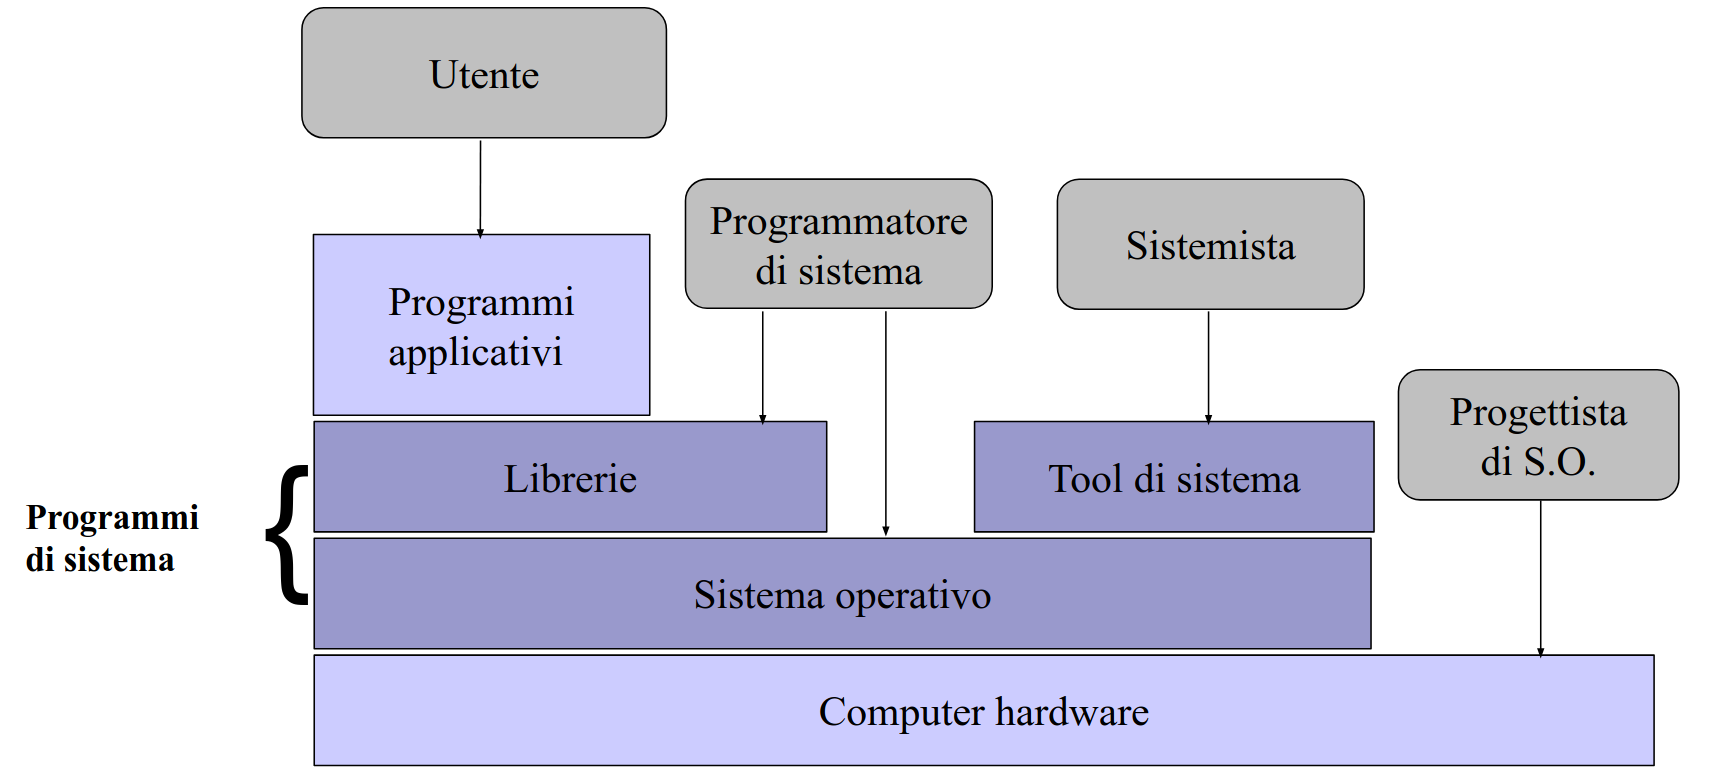
\includegraphics[width=0.7\linewidth]{Images/Screenshot 2024-12-15 at 18-55-32 so-01-intro-os.pptx - so-01-intro-os.pdf.png}
    \caption{Un S.O nasconde ai programmatori i dettagli dell'hardware e fornisce ai programmatori una API conveniente e facile da usare, agisce come intermediario tra programmatore e hardware.}
     \label{fig:Figura1}
\end{figure}

\textbf{S.O come macchina estesa}

\begin{multicols}{2}
   \begin{lstlisting}
//Esempio senza S.O.
li $t0, 0xDEFF12 // init
sw $t0, 0xB000.0040
li $t0, 0xFFDF // motor
sw $t0, 0xB000.0044
li $t0, 0xFFBB
sw $t0, 0xBOOO.0048
...
\end{lstlisting}
    \columnbreak
    \begin{lstlisting}[language=]
//Esempio con S.O.
fd = open("/etc/rpc");
read(fd, buffer, size);
\end{lstlisting}
\end{multicols}

\begin{center}
    \small\textit{NB: Questo è esempio serve a dare un'idea,
la realtà è molto più complessa \dots}
\end{center}

\paragraph{Servizi estesi offerti da un S.O.}
\begin{itemize}
\item[-] esecuzione di programmi
\item[-] accesso semplificato ai dispositivi di I/O
\item[-] accesso controllato a dispositivi, file system, etc.
\item[-] accesso al sistema
\item[-] rilevazione e risposta agli errori
\item[-] accounting
\end{itemize}

\subsection{Tipi di sistemi}

\subsubsection{Sistemi Paralleli}
\textbf{Definizione:} Un sistema parallelo è un singolo elaboratore che possiede più unità di elaborazione. Si dicono anche sistemi tightly coupled.
Alcune risorse contenute nell'elaboratore possono essere condivise.
\textit{Esempio: Memoria}
La comunicazione avviene tramite memoria condivisa o canali di
comunicazione dedicati.

\paragraph{Vantaggi dei sistemi paralleli}
    \begin{itemize}
        \item incremento delle prestazioni
        \item incremento dell’affidabilità (graceful degradation)
    \end{itemize}

\paragraph{Tassonomia basata sulla struttura}
 \begin{itemize}
\item \textbf{SIMD} - Single Instruction, Multiple Data: Le CPU              eseguono all'unisono lo stesso programma su dati diversi
\item \textbf{MIMD} - Multiple Instruction, Multiple Data: Le CPU            eseguono programmi differenti su dati differenti
\end{itemize}

\paragraph{Tassonomia basata sulla dimensione}

A seconda del numero (e della potenza) dei processori si suddividono in:
\begin{itemize}
\item sistemi a basso parallelismo
pochi processori in genere molto potenti
\item sistemi massicciamente paralleli
gran numero di processori, che possono avere anche potenza non elevata
\end{itemize}

\subsubsection{Sistemi Distribuiti}
\textbf{Definizione:} Sono sistemi composti da più elaboratori indipendenti (con proprie risorse e
proprio sistema operativo)
Si dicono anche sistemi loosely coupled.
Ogni processore possiede la propria memoria locale e sono collegati tramite linee di comunicazione (rete, linee
telefoniche, linee wireless, etc)

\paragraph{Vantaggi dei sistemi distribuiti}
    \begin{itemize}
    \item Condivisione di risorse
    \item Suddivisione di carico, incremento delle prestazioni
    \item Affidabilità
    \item Possibilità di comunicare
\end{itemize}

I Sistemi operativi di rete forniscono condivisione di file, la possibilità di comunicare e ogni computer opera indipendentemente dagli altri.

I Sistemi operativi distribuiti offrono minore autonomia tra i computer e danno l'impressione che un singolo sistema operativo stia controllando la rete

\subsubsection{Sistemi real-time}
\textbf{Definizione:} Sono i sistemi per i quali la correttezza del risultato non dipende solamente dal suo valore ma anche dall'istante nel quale il risultato viene prodotto

I sistemi real-time si dividono in:
\begin{itemize}
    \item hard real-time: se il mancato rispetto dei vincoli temporali può avere effetti catastrofici. \textit{e.g. controllo assetto velivoli, controllo centrali nucleari.}
    \item soft real-time: se si hanno solamente disagi o disservizi \textit{e.g. programmi interattivi}
\end{itemize}

\newpage
\section{Concetti base di architetture
degli elaboratori}

\begin{figure} [h]
    \centering
    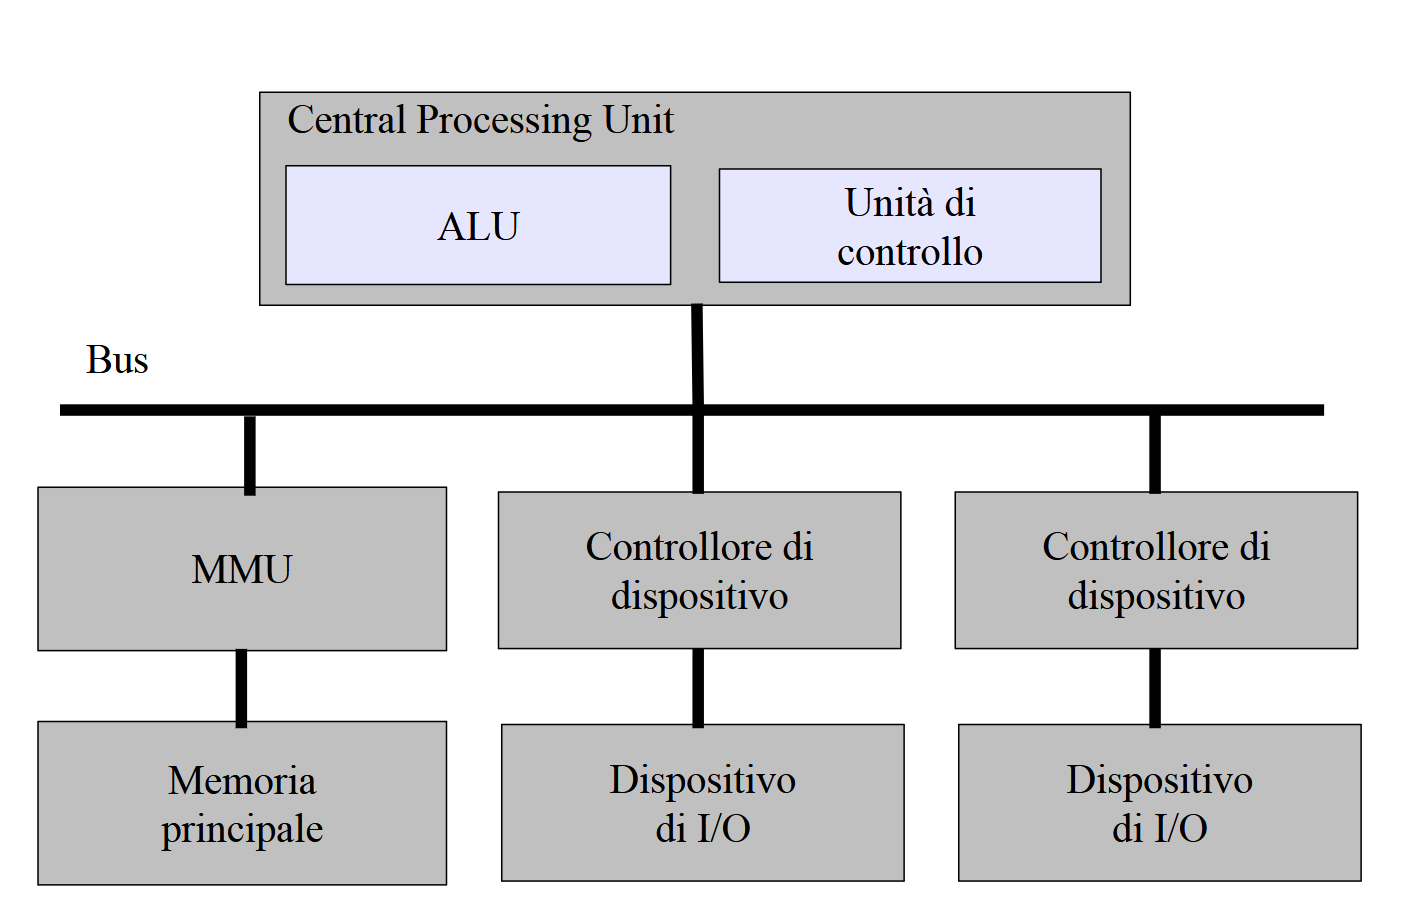
\includegraphics[width=0.5\linewidth]{Images/Screenshot 2024-12-16 125618.png}
    \caption{Architettura di Von Neumann}
    \label{fig:von-neumann1}
\end{figure}

\subsection{Interrupt}
\textbf{Definizione:} Un meccanismo che permette l'interruzione del normale ciclo di esecuzione della CPU.

Le caratteristiche: introdotti per aumentare l'efficienza di un sistema di calcolo, permettono ad un S.O. di "intervenire" durante l'esecuzione di un processo utente, allo scopo di gestire efficacemente le risorse del calcolatore.
\textit{Esempio:} processore, memoria, dispositivi di I/O

Gli interrupt possono essere sia hardware che software (detti \underline{trap})
e possono essere mascherati (ritardati) se la CPU sta svolgendo compiti non interrompibili.

\subsubsection{Interrupt vs Trap}

\begin{itemize}
    \item[-] Interrupt Hardware: eventi hardware asincroni, non causati dal processo in esecuzione

\textit{Esempi: dispositivi di I/O
(per notifica di eventi quali il completamento di una operazione di I/O), clock (scadenza del quanto di tempo)}
\item[-] Interrupt Software (Trap): Causato dal programma

\textit{Esempi: eventi eccezionali come divisione per 0 o problemi di indirizzamento, richiesta di servizi di sistema.(system call)}
\end{itemize}

\subsubsection{Gestione Interrupt - Panoramica}
Cosa succede in seguito ad un interrupt.
\newline

\textbf{Dal lato software:}
\begin{enumerate}
    \item Un segnale "interrupt request" viene spedito al processore.
    \item Il processore sospende le operazioni del processo corrente e salta ad un particolare indirizzo di memoria contenente la routine di gestione dell'interrupt (\underline{interrupt handler}).
\end{enumerate}




\textbf{Dal lato hardware}
\begin{enumerate}
    \item L'interrupt handler gestisce nel modo opportuno l'interrupt e ritorna il controllo al processo interrotto (o a un altro processo, nel caso di scheduling).
    \item Il processore riprende l'esecuzione del processo interrotto come se nulla fosse successo
\end{enumerate}
\newpage
\begin{figure} [h]
    \centering
    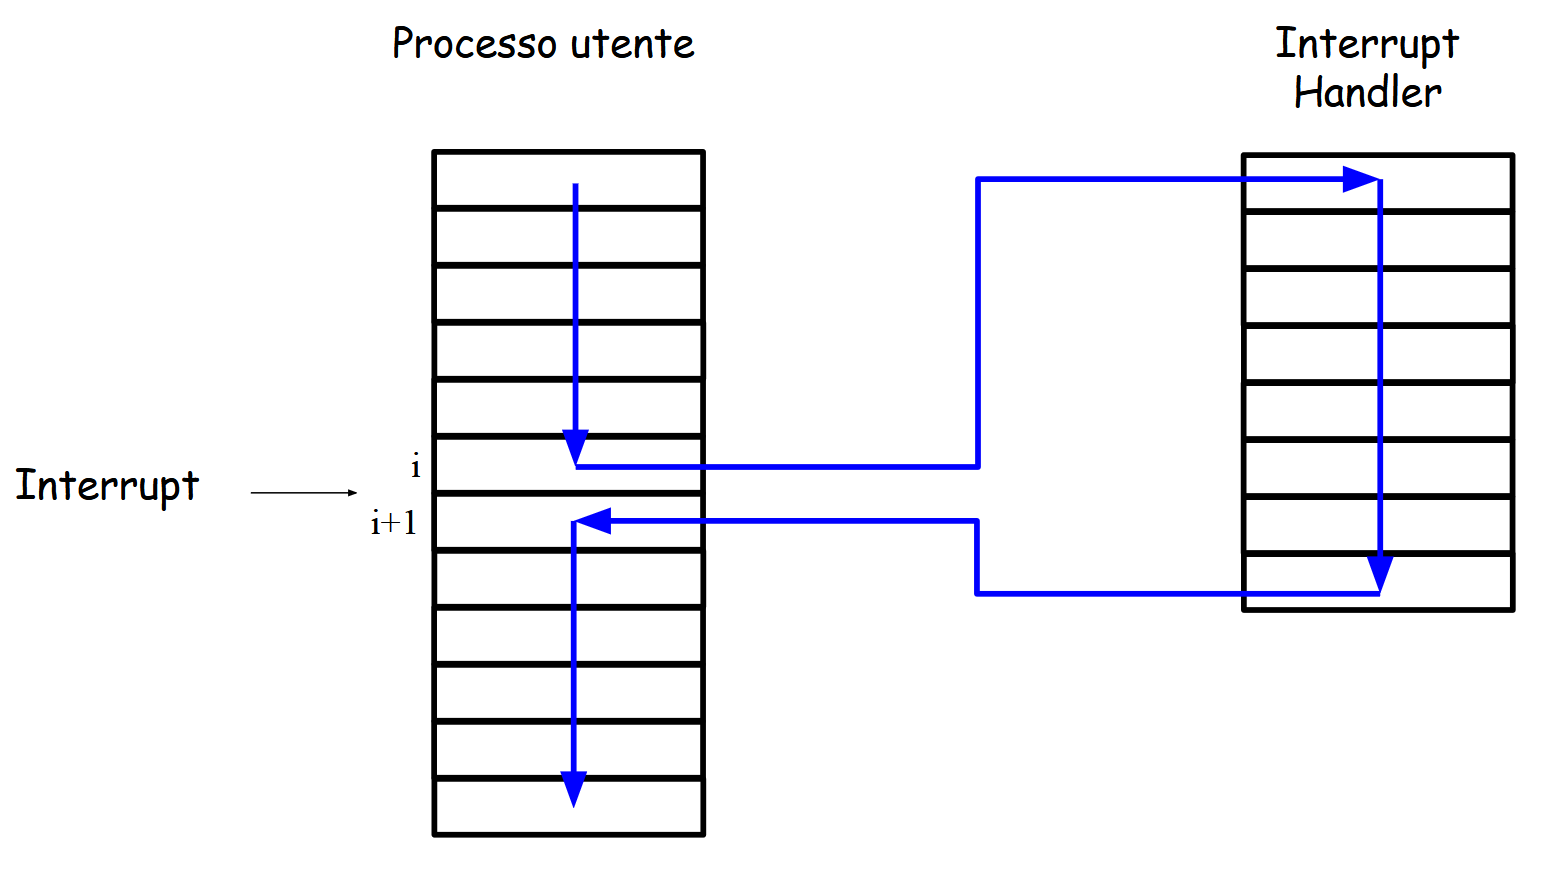
\includegraphics[width=0.7\linewidth]{Images/Screenshot 2024-12-16 132614.png}
    \label{fig:interrupt1}
\end{figure}

\subsubsection{Gestione Interrupt - Dettagli}

\begin{enumerate}
    \item Un segnale di interrupt request viene spedito alla CPU.
    \item La CPU finisce l'esecuzione dell'istruzione corrente.
    \item La CPU verifica la presenza di un segnale di interrupt, e
in caso affermativo spedisce un segnale di conferma al device
che ha generato l'interrupt.

\begin{figure} [h]
    \centering
    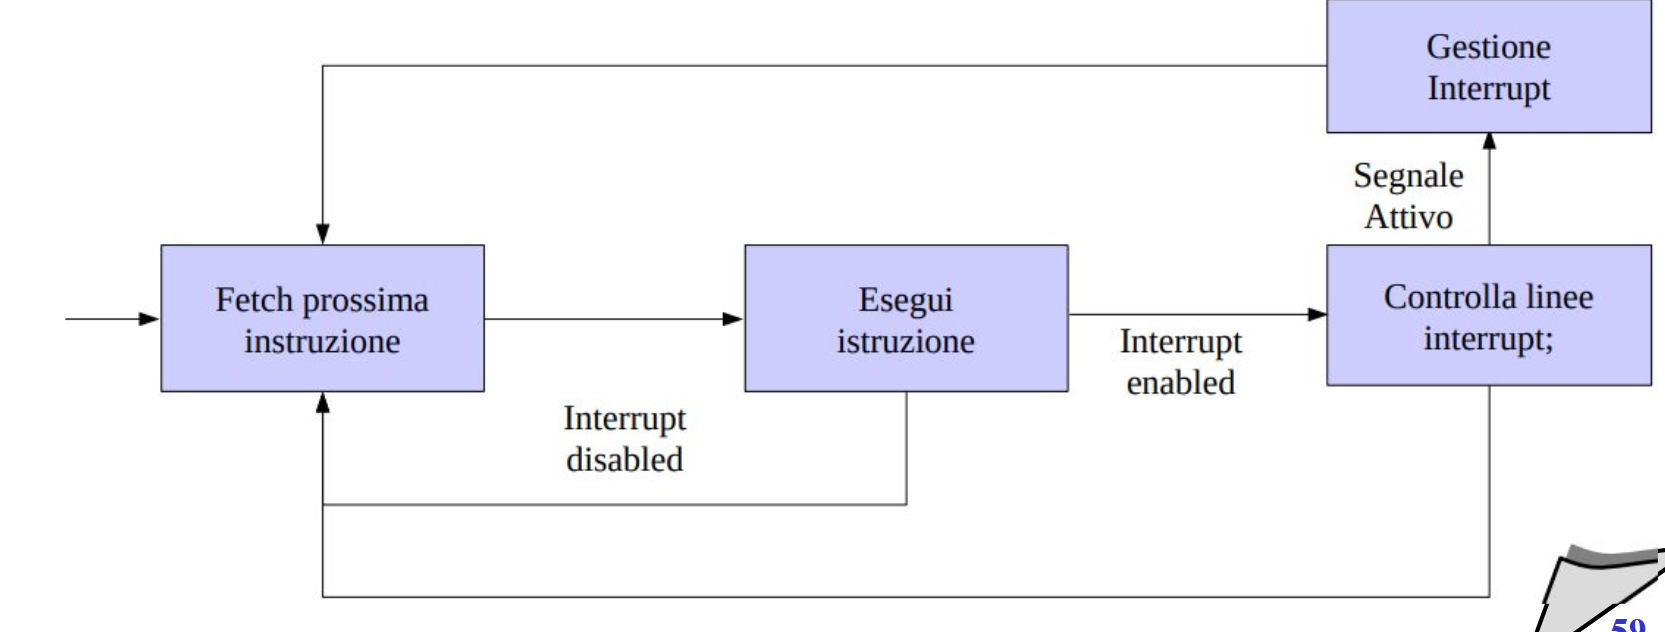
\includegraphics[width=0.7\linewidth]{Images/Screenshot 2024-12-16 132946.png}
    \label{fig:enter-label}
\end{figure}

\item  Preparazione al trasferimento di controllo dal programma all'interrupt handler
\item Selezione dell'interrupt handler appropriato a seconda dell'architettura, vi può essere un singolo interrupt handler,
uno per ogni tipo di interrupt o uno per dispositivo. La selezione avviene tramite l'interrupt vector.
\item Caricamento del PC con l'indirizzo iniziale dell'interrupt handler assegnato.

\small \textit{Nota: tutte le operazioni compiute fino a qui sono operazioni hardware, la modifica del PC corrisponde ad un salto al codice dell'interrupt handler.
A questo punto: il ciclo fetch-execute viene ripreso il controllo è passato in mano all'interrupt handler.}
\item Salvataggio dello stato del processore: salvataggio delle informazioni critiche non salvate automaticamente
dai meccanismi hardware di gestione interrupt.
\item Gestione dell'interrupt: 
lettura delle informazioni di controllo proveniente dal dispositivo. Eventualmente, spedizione di ulteriori informazioni al dispositivo stesso.
\item Ripristino dello stato del processore
l'operazione inversa della numero 7.
\item Ritorno del controllo al processo in esecuzione
(o ad un altro processo, se necessario).


\end{enumerate}


\subsubsection{Interrupt Multipli}
 La discussione precedente prevedeva la presenza di un singolo
interrupt.
Esiste la possibilità che avvengano interrupt multipli ad esempio, originati da dispositivi diversi, un interrupt può avvenire durante la gestione di un interrupt precedente.
\newline
Esistono due approcci possibili: disabilitazione degli interrupt e interrupt annidati.
\newline

\textbf{Disabilitazione Interrupt:}
durante l'esecuzione di un interrupt handler ulteriori segnali di interrupt vengono ignorati, i segnali corrispondenti restano pendenti. Gli interrupt vengono riabilitati prima di riattivare il processo interrotto e il processore verifica quindi se vi sono ulteriori interrupt, in caso attiva l'interrupt handler corrispondente.
\newline

\underline{Vantaggi e svantaggi:}
\newline
Approccio semplice, interrupt gestiti in modo sequenziale,  non tiene conto di gestioni "time-critical".

\begin{figure} [h]
    \centering
    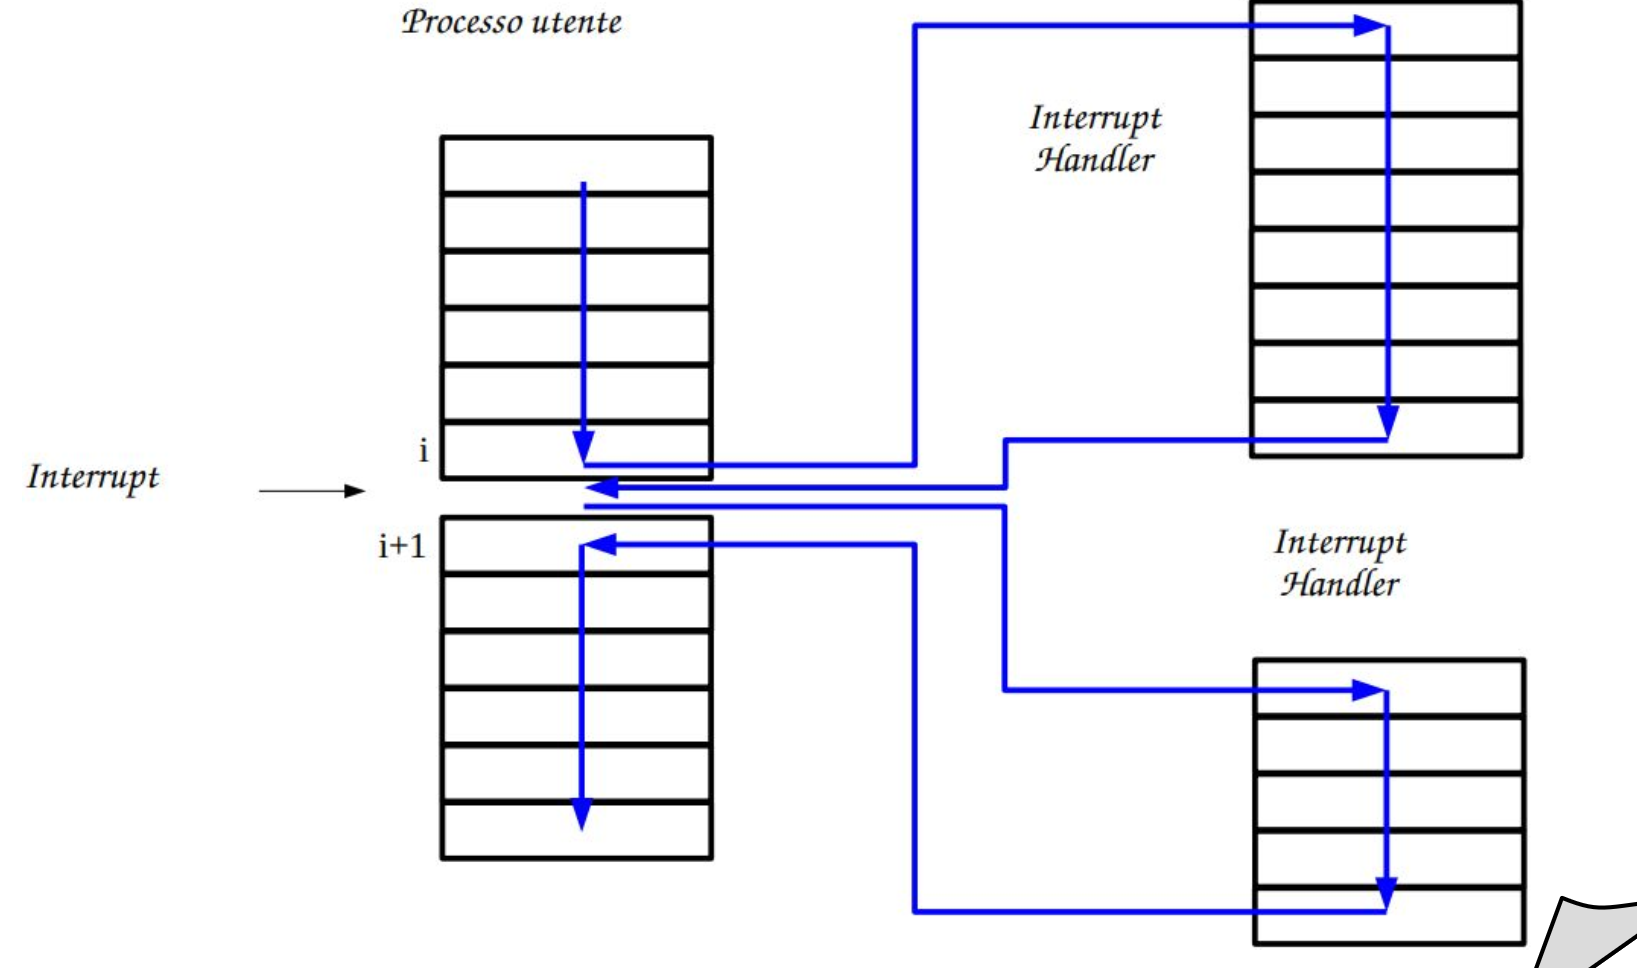
\includegraphics[width=0.7\linewidth]{Images/Screenshot 2024-12-16 140040.png}
    \label{fig:enter-label}
\end{figure}

\textbf{Interrupt Annidati:}
E' possibile definire priorità diverse per gli interrupt. Un interrupt di priorità inferiore può essere interrotto da un interrupt di priorità superiore. Necessario prevedere un meccanismo di salvataggio e ripristino dell'esecuzione adeguato.
\newline

\underline{Vantaggi e svantaggi:}
\newline
dispositivi veloci possono essere serviti prima (es. schede di rete), approccio più complesso.

\begin{figure} [h]
    \centering
    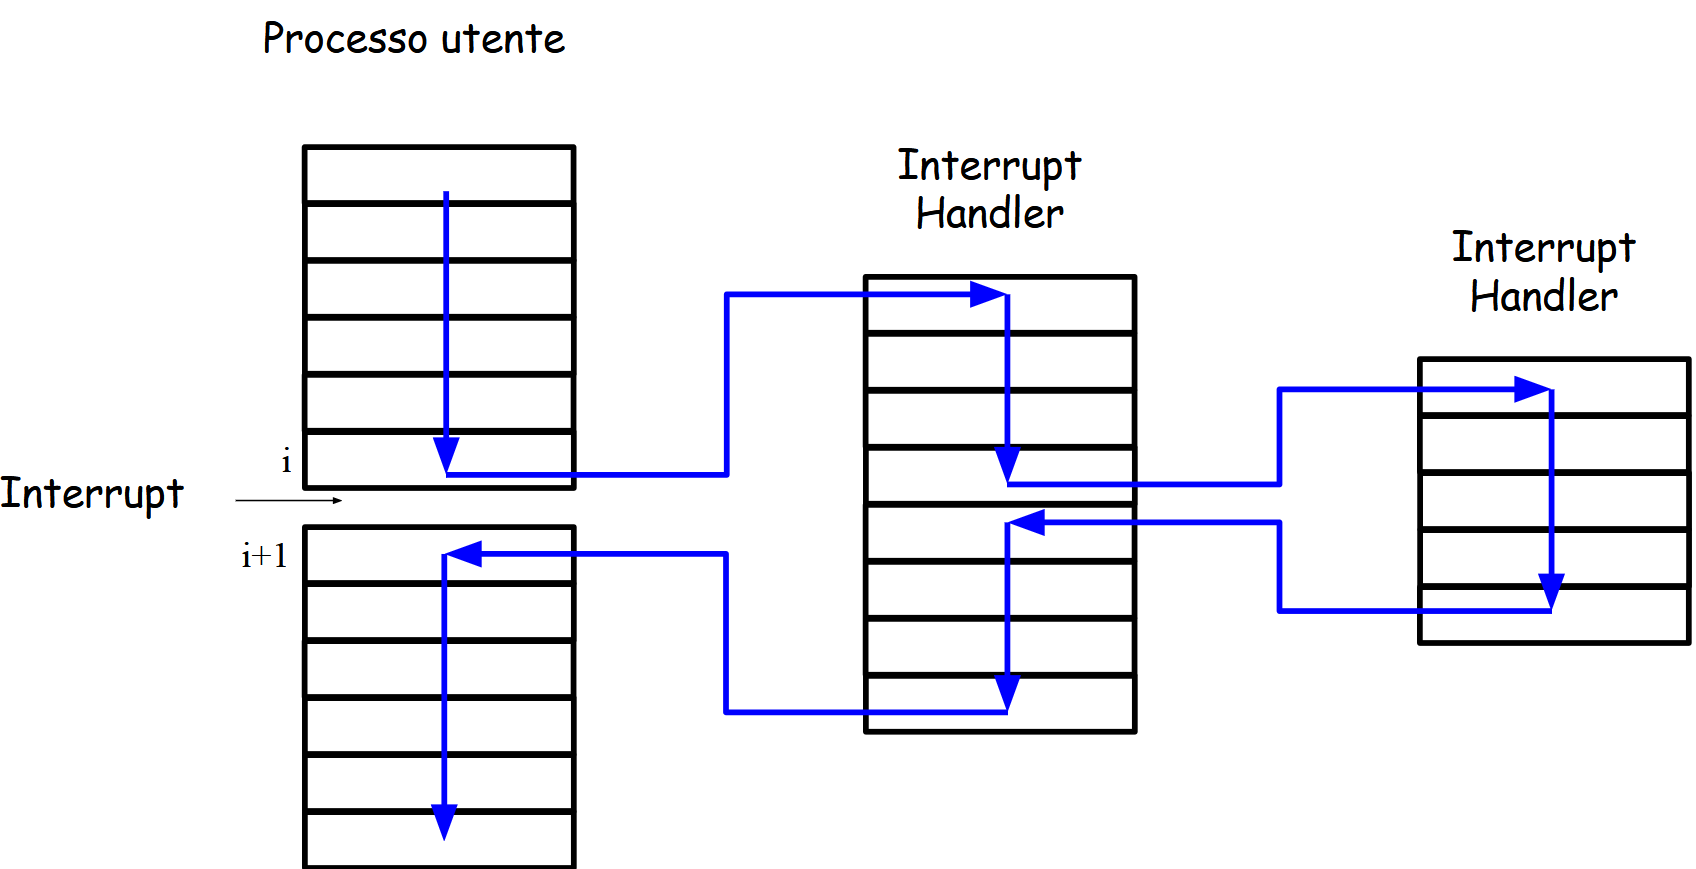
\includegraphics[width=0.7\linewidth]{Images/Screenshot 2024-12-16 140334.png}

    \label{fig:enter-label}
\end{figure}

\subsection{Comunicazione fra processore e dispositivi di I/O}
Il controllore governa il dialogo con il dispositivo fisico, il controllo della politica di accesso al dispositivo è a carico del dispositivo stesso

\textit{Esempio:
il controller di un disco accetta una richiesta per volta, 
l'accodamento delle richieste in attesa è a carico del S.O.}
\newline

Esistono 3 modalità di controllo;
\begin{enumerate}
    \item Programmed I/O
    \item Interrupt-Driven I/O
    \item Direct Memory Access (DMA)
\end{enumerate}

\subsubsection{Programmed I/O (obsoleto)}
\textbf{Operazione di input:}
\newline
La CPU carica (tramite il bus) i parametri della richiesta di input in appositi registri del controller (registri comando).

Il dispositivo esegue la richiesta, il risultato dell'operazione viene memorizzato in un apposito buffer locale sul controller. Il completamento dell'operazione viene segnalato attraverso appositi registri di status.

Il S.O. attende (busy waiting) che il comando sia completato
verificando periodicamente il contenuto del registro di stato.

Infine, la CPU copia i dati dal buffer locale del controller alla memoria.

\subsubsection{Interrupt-Driven I/O}
\textbf{Operazione di input:}
\newline
La CPU carica (tramite il bus) i parametri della richiesta di input in appositi registri del controller (registri comando).

Il S.O. sospende l'esecuzione del processo che ha eseguito
l'operazione di input ed esegue un altro processo.

Il dispositivo esegue la richiesta, il risultato dell'operazione viene memorizzato in un apposito buffer locale sul controller, il completamento dell'operazione viene segnalato attraverso interrupt.

Al ricevimento dell'interrupt, la CPU copia i dati dal buffer locale del controller alla memoria.

\subsubsection{Programmed I/O vs Interrupt-Driven I/O}
Nel caso di operazioni di output il procedimento è similare:
\begin{itemize}
    \item i dati vengono copiati dalla memoria ai buffer locali.
    \item questa operazione viene eseguita prima di caricare i parametri della richiesta nei registri di comando dei dispositivi.
\end{itemize}

\textbf{Svantaggi dei due approcci:}
\begin{itemize}
    \item il processore spreca parte del suo tempo nella gestione del trasferimento dei dati.
    \item la velocità di trasferimento è limitata dalla velocità con cui il processore riesce a gestire il servizio.
\end{itemize}

\subsubsection{Direct Memory Access (DMA)}

Il S.O. attiva l'operazione di I/O specificando l'indirizzo in memoria di destinazione (Input) o di provenienza (Output) dei dati.

L'interrupt specifica solamente la conclusione dell'operazione di I/O.
\newline

\textbf{Vantaggi e svantaggi:}
\begin{itemize}
    \item c'è contesa nell'accesso al bus device driver più semplici.
    \item efficace perché la CPU non accede al bus ad ogni ciclo di clock.
\end{itemize}

\subsection{Memoria}
\subsubsection{Memory Mapped I/O}
Un dispositivo è completamente indirizzabile tramite bus.
I registri di dispositivo vengono mappati su un insieme di indirizzi di memoria, una scrittura su questi indirizzi causa il trasferimento di dati verso il dispositivo.
\textit{Esempio: video grafico nei PC.}
\newline

\textbf{Vantaggi e svantaggi:}
\begin{itemize}
    \item gestione molto semplice e lineare.
    \item necessità di tecniche di polling.
\end{itemize}
\subsubsection{Dischi}
Sono dispositivi che consentono la memorizzazione non volatile dei dati permettono accesso diretto. Per individuare un dato sul disco (dal punto di vista fisico) occorre indirizzarlo in termini di cilindro, testina, settore.

Le operazioni gestite dal controller sono: READ (head, sector), WRITE(head, sector), SEEK(cylinder).

L'operazione di seek:
Corrisponde allo spostamento fisico del pettine di testine da
un cilindro ad un altro ed è normalmente la più costosa

L'operazione di read e write:
prevedono l'attesa che il disco ruoti fino a quando il settore richiesto raggiunge la testina.

\subsubsection{Gerarchia di memoria}
Trade off: Quantità, velocità, costo.
\newline
Limitazioni:
\begin{itemize}
    \item tempo di accesso più veloce, costo maggiore.
    \item maggiore capacità, costo minore (per bit).
    \item maggiore capacità, tempo di accesso maggiore.
\end{itemize}
Soluzione: utilizzare una gerarchia di memoria.
\begin{figure}[h]
    \centering
    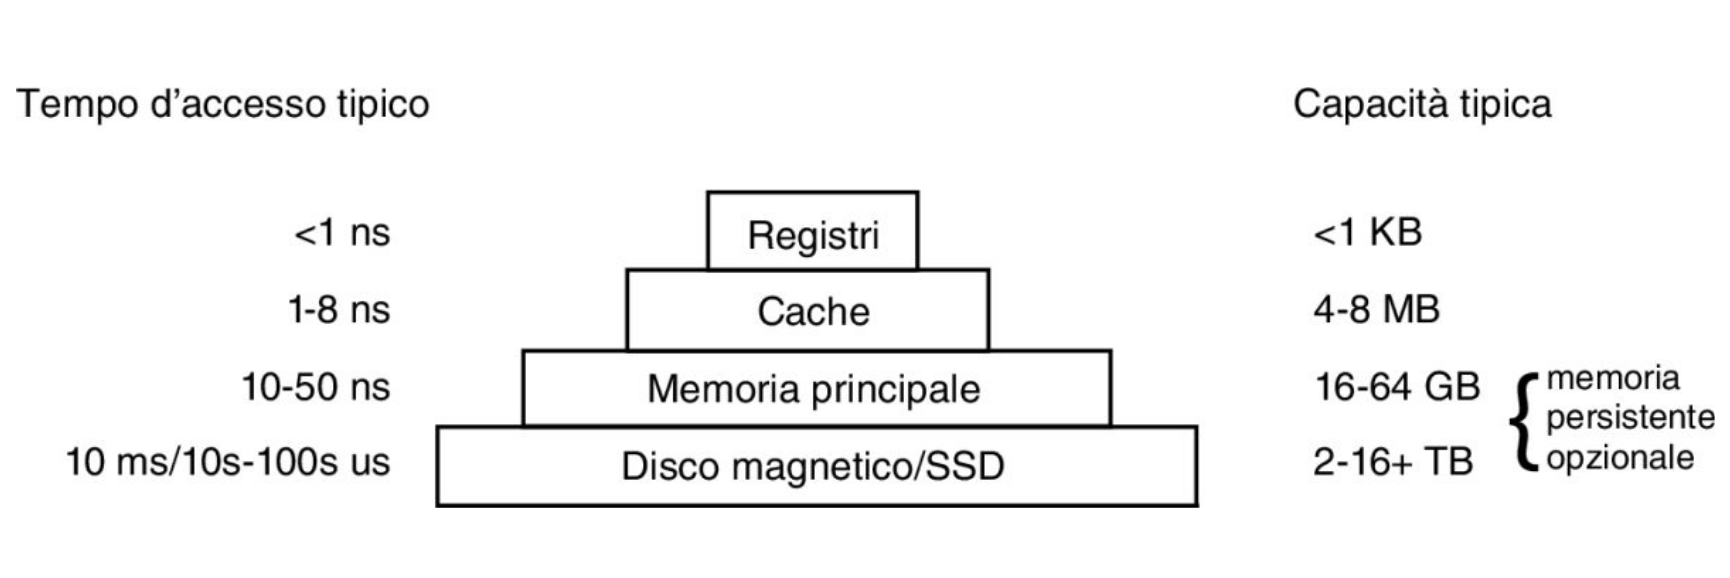
\includegraphics[width=0.7\linewidth]{Images/Screenshot 2024-12-17 at 19-02-22 so-01-intro-os.pptx - so-01-intro-os.pdf.png}
    \label{fig:enter-label}
\end{figure}

\subsubsection{Cache}
Un meccanismo di caching consiste nel memorizzare parzialmente i dati di una memoria in una
seconda più costosa ma più efficiente. Se il numero di occorrenze in cui il dato viene trovato nella cache
(memoria veloce) è statisticamente rilevante rispetto al numero totale degli accessi, la cache fornisce un notevole aumento di prestazione.

E' un concetto che si applica a diversi livelli: cache della memoria principale (DRAM), cache di disco in memoria, cache di file system remoti tramite file system locali.

I meccanismi di caching si distinguono in due modi:
\begin{itemize}
    \item \textbf{Hardware} ad esempio cache CPU; politiche non modificabili dal S.O.
    \item \textbf{Software} ad esempio cache disco; politiche sotto controllo del S.O.
\end{itemize}
I problemi da considerare nel S.O. sono molteplici. Come l' algoritmo di replacement, data la dimensione limitata della cache bisogna scegliere un algoritmo che garantisca il maggior numero di accessi in cache. Oppure la coerenza, gli stessi dati possono apparire a diversi livelli della struttura di memoria.

\subsection{Protezione Hardware}
I sistemi multiprogrammati e multiutente richiedono la presenza di meccanismi di protezione. Bisogna evitare che processi concorrenti generino interferenze non
previste, ma soprattutto bisogna evitare che processi utente interferiscano con il sistema operativo.

Quindi i meccanismi di protezione possono essere realizzati totalmente in software, oppure abbiamo bisogno di meccanismi hardware dedicati?
\newpage
\subsubsection{Modo utente / Modo kernel}
\paragraph{Modalità kernel / supervisore / privilegiata:}
I processi in questa modalità hanno accesso a tutte le istruzioni, incluse quelle privilegiate, che permettono di gestire totalmente il sistema.
\paragraph{Modalità utente:} 
I processi non hanno accesso alle istruzioni privilegiate.
\newline
Il mode bit è un bit utilizzato nei processori per distinguere tra due modalità operative: modalità kernel e modalità utente.

\paragraph{Come funziona?}
Alla partenza, il processore è in modalità kernel.
Viene caricato il sistema operativo (bootstrap) e si inizia ad eseguirlo, quando passa il controllo ad un processo utente, il S.O. cambia il valore del mode bit e il processore passa in modalità utente.
Tutte le volte che avviene un interrupt, l'hardware passa da modalità utente a modalità kernel.

\subsubsection{Protezione I/O}
Le istruzioni di I/O devono essere considerate privilegiate, il S.O. dovrà fornire agli utenti primitive e servizi per accedere all'I/O. Tutte le richieste di I/O passano attraverso codice del S.O. e possono essere controllate preventivamente.
\textit{Esempio: accesso al dispositivo di memoria secondaria che ospita un file system. Vogliamo evitare che un qualunque processo possa accedere al dispositivo modificando (o corrompendo) il file system stesso.}

\subsubsection{Protezione Memoria}
La protezione non è completa se non proteggiamo anche la
memoria, altrimenti, i processi utente potrebbero: modificare il codice o i dati di altri processi utenti, modificare il codice o i dati del sistema operativo, modificare l'interrupt vector, inserendo i propri gestori degli interrupt.

La protezione avviene tramite la \textbf{Memory Management Unit(MMU).}

\paragraph{Registro base + registro limite:} ogni indirizzo generato dal processore viene confrontato con due registri,
detti base e limite. Se non incluso in questo range, l'indirizzo non è valido e genera un'eccezione.
\paragraph{Traduzione indirizzi logici in indirizzi fisici:} ogni indirizzo generato dal processore corrisponde ad un indirizzo logico, l'indirizzo logico viene trasformato in un indirizzo fisico a tempo di esecuzione dal meccanismo di MMU.
Un indirizzo viene protetto se non può mai essere generato
dal meccanismo di traduzione.

\begin{figure} [h]
    \centering
    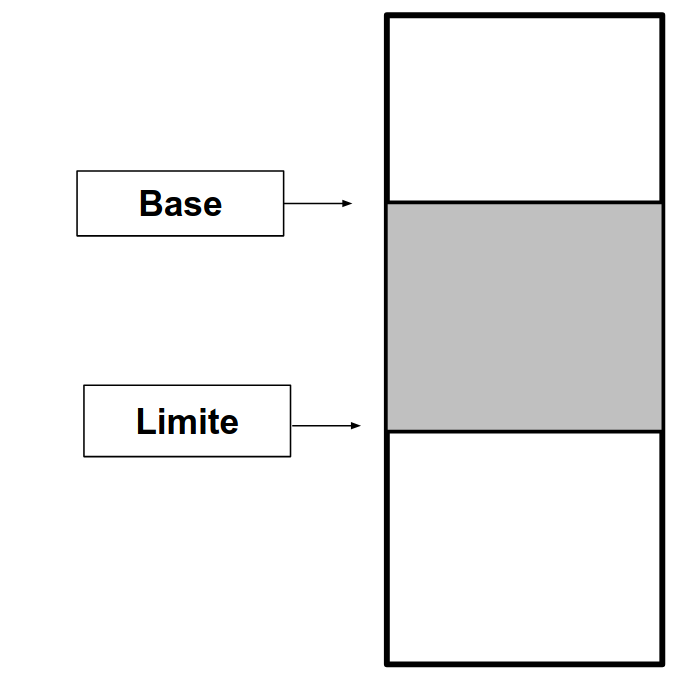
\includegraphics[width=0.3\linewidth]{Images/Screenshot 2024-12-17 at 19-31-43 so-01-intro-os.pptx - so-01-intro-os.pdf.png}
    \label{fig:enter-label}
\end{figure}

\newpage
\section{Struttura dei sistemi operativi
(panoramica)}

\subsection{Architettura dei sistemi operativi}
L'architettura di un sistema operativo descrive quali sono le varie componenti del S.O. e come queste sono
collegate fra loro. I vari sistemi operativi sono molto diversi l'uno dall'altro nella loro architettura, la progettazione di essa è un problema fondamentale.

L'architettura di un S.O. da diversi punti di vista:
servizi forniti (visione utente), interfaccia di sistema (visione programmatore), componenti del sistema (visione progettista S.O.)

\subsubsection{Le componenti di un S.O:}
\begin{enumerate}
    \item Gestione dei processi
    \item Gestione della memoria principale
    \item Gestione della memoria secondaria
    \item Gestione file system
    \item Gestione dei dispositivi di I/O
    \item Protezione
    \item Networking
    \item Interprete dei comandi
\end{enumerate}

\paragraph{Gestione dei processi}
Un processo è un programma in esecuzione che utilizza le risorse fornite dal computer per assolvere i propri compiti.

Il sistema operativo è responsabile delle seguenti attività riguardanti la gestione dei processi: creazione e terminazione dei processi, sospensione e riattivazione dei processi, gestione dei deadlock, comunicazione tra processi
e sincronizzazione tra processi.

\paragraph{Gestione della memoria principale}
La memoria principale è un "array" di byte indirizzabili singolarmente. Consideriamolo un deposito di dati facilmente accessibile e condiviso tra la CPU ed i dispositivi di I/O.

Il sistema operativo è responsabile delle seguenti attività
riguardanti la gestione della memoria principale: tenere traccia di quali parti della memoria sono usate e da chi, decidere quali processi caricare quando diventa disponibile spazio in memoria e allocare e deallocare lo spazio di memoria quando necessario.

\paragraph{Gestione della memoria secondaria}
Poiché la memoria principale è volatile e troppo piccola per contenere tutti i dati e tutti i programmi in modo permanente, un computer è dotato di memoria secondaria.
In generale, la memoria secondaria è data da hard disk, dischi ottici, nastri, etc.

Il sistema operativo è responsabile delle seguenti attività
riguardanti la gestione della memoria secondaria: Allocazione dello spazio inutilizzato, Gestione dello spazio di memorizzazione e ordinamento efficiente delle richieste (disk scheduling).

\paragraph{Gestione file system}
Un file è l'astrazione informatica di un archivio di dati.
Il concetto di file è indipendente dal media sul quale viene
memorizzato (che ha caratteristiche proprie e propria organizzazione fisica). Un file system è composto da un insieme di file. 

Il sistema operativo è responsabile delle seguenti attività
riguardanti la gestione del file system: creazione e cancellazione di file, creazione e cancellazione di directory, manipolazione di file e directory e codifica del file system sulla memoria secondaria.

\paragraph{Gestione dei dispositivi di I/O}
La gestione dell’I/O richiede: un’interfaccia comune per la gestione dei device driver, un insieme di driver per dispositivi hardware specifici e un sistema di gestione di buffer per il caching delle informazioni.

\paragraph{Protezione}
Il termine protezione si riferisce al meccanismo per controllare gli accessi di programmi, processi o utenti alle risorse del sistema e degli utenti.

Il meccanismo di protezione software deve: distinguere tra uso autorizzato o non autorizzato, specificare i controlli che devono essere imposti e fornire un meccanismo di attuazione della protezione.

\paragraph{Networking}
Consente di far comunicare due o più elaboratori, condividere risorse, utilizzando servizi come: protocolli di comunicazione a basso livello, TCP/IP, UDP, comunicazione ad alto livello, file system distribuiti (NFS, SMB) e print spooler.

\paragraph{Interprete dei comandi}
Interfaccia utente - S.O. .
Può attivare un programma, terminare un programma, interagire con le componenti del sistema operativo (file system).
Può essere: grafica (a finestre, icone, etc.), testuale (linea di comando).
Può cambiare il "linguaggio" utilizzato, ma il concetto è lo stesso, d'altronde vi sono differenze di espressività
\newline
\small\textit{N.B L'interprete dei comandi usa i servizi dei gestori di processi, I/O, memoria principale e secondaria}

\subsection{System Call}

\subsubsection{Cos'è la system call}
\paragraph{Problema:} poiché le istruzioni di I/O sono privilegiate, possono essere eseguite unicamente dal S.O. . Com'è possibile per i processi utenti eseguire operazioni di I/O?
\paragraph{Soluzione:} i processi utenti devono fare richieste esplicite di I/O al S.O. . Questo introduce il meccanismo delle system call, ovvero trap generate da istruzioni specifiche.
\newline

Ogni volta che un processo ha bisogno di un servizio del S.O.
richiama una system call. Sono in genere disponibili come istruzioni a livello assembler, esistono librerie che permettono di invocare le system call da diversi linguaggi \textit{(ad es. librerie C)}.
Vengono normalmente realizzate tramite interrupt software.
Le system call sono specifiche dei vari sistemi operativi.
\newline

Esempi di istruzioni privilegiate eseguibili in Kernel Mode:
\small\begin{itemize}
    \item Gestione della memoria
    \item Gestione della memoria virtuale (allocazione, etc.)
    \item Controllo dell'hardware (I/O, controller di interrupt)
    \item Gestione della CPU
    \item Istruzioni di halt e riavvio
    \item Gestione del clock di sistema
    \item Operazioni sulla cache
    \item Gestione dell'alimentazione
    \item Operazioni crittografiche hardware
    \item Gestione delle eccezioni e degli interrupt
    \item Accesso a registri di controllo speciali
    \item \dots
\end{itemize}





\subsubsection{Gestione dei file}

\begin{lstlisting} 
    pid = fork() //crea un processo figlio identico al padre
\end{lstlisting}

\begin{lstlisting} 
    pid = waitpid(pid, &statloc, options) //aspetta la terminazione di un processo figlio
\end{lstlisting}

\begin{lstlisting} 
    s = execve(name, argv, environment) //esegue un programma
\end{lstlisting}

\begin{lstlisting} 
    exit(status) //termina l'esecuzione del processo corrente
\end{lstlisting}

\begin{lstlisting} 
//Un programma che genera un processo figlio:
int main(void) {
    int pid;
    pid = fork();
    if (pid > 0) {
        printf('Padre\n');
    } else if (pid == 0) {
        printf('Figlio\n');
    } else {
        printf('Errore!\n');
    }
}
\end{lstlisting}

\subsubsection{Gestione del file system e delle directory}
\begin{lstlisting}
  s = mkdir(name, mode) //Crea una nuova directory  
\end{lstlisting}

\begin{lstlisting}
  s = rmdir(name) //Cancella una directory 
\end{lstlisting}

\begin{lstlisting}
  s = link(name1, name2) //Crea un nuovo link ad un file esistente
\end{lstlisting}

\begin{lstlisting}
 s = unlink(name) //Cancella un file  
\end{lstlisting}

\begin{lstlisting}
   s = mount(special, name, flag) //Monta una partizione nel file system
\end{lstlisting}

\begin{lstlisting}
   s = umount(special) //Smonta una partizione
\end{lstlisting}

\subsubsection{Varie}

\begin{lstlisting}
   s = chdir(dirname) //Cambia la directory corrente
\end{lstlisting}

\begin{lstlisting}
   s = chmod(name, mode) //Cambi i bit di protezione di un file
\end{lstlisting}

\begin{lstlisting}
   s = kill(pid, signal) //Spedisce un segnale ad un processo
\end{lstlisting}

\begin{lstlisting}
   seconds = time(&seconds) //Restituisce il tempo di sistema
\end{lstlisting}
\newpage
\subsection{File Speciali (UNIX)}
I file speciali sono pensati per far sì che i dispositivi di I/O siano visti come file.
\paragraph{I file speciali a blocchi:}
usati per modellare dispositivi costituiti da un insieme di blocchi indirizzabili in modo casuale (SSD, dischi). Aprendo un file speciale a blocchi e leggendo il blocco 4, un programma può accedere direttamente al quarto blocco, senza considerare la struttura del file system
\paragraph{I file speciali a caratteri:}
usati per modellare stampanti, tastiere, mouse, etc. che accettano una sequenza di caratteri in output, contenuti nella directory /dev.

\subsubsection{Pipe}
Una pipe è una specie di pseudo-file che può essere usato per
connettere due processi.
\begin{figure}[h]
    \centering
    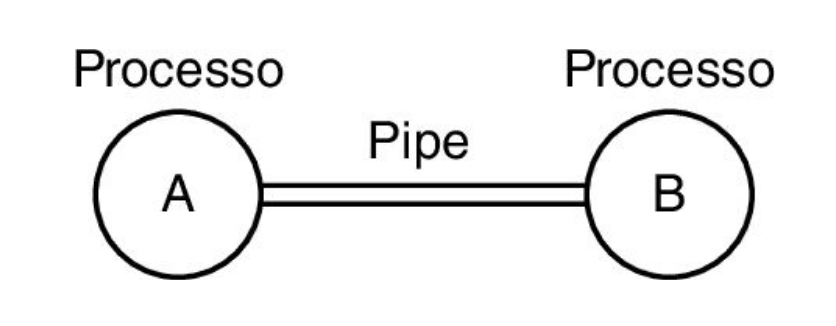
\includegraphics[width=0.4\linewidth]{Images/Screenshot 2024-12-18 at 13-24-07 so-01-intro-os.pptx - so-01-intro-os.pdf.png}
    \label{fig:enter-label}
\end{figure}

\paragraph{Pipe in Bash:} Le abbiamo viste con Ghini.
\textit{Esempio: A $||$ B}

\paragraph{Pipe in C:} Utilizza la funzione pipe() e i descrittori di file, permette la comunicazione tra processi correlati (es. genitore-figlio). Sono unidirezionali (ma possono essere create multiple pipe per bidirezionalità)
La creazione è esplicita nel codice del programma e persiste finché non viene chiusa o il processo termina.
\textit{Esempio:
pipe(pipefd)
… write(pipefd[1], ...)
… read(pipefd[0], …)}

\chapter{Scheduling}
\newpage

\section{Scheduler, Processi e Thread}
\subsection{Introduzione}
Un sistema operativo è un gestore di risorse come: processore, memoria principale e secondaria, dispositivi. Per svolgere i suoi compiti, un sistema operativo ha bisogno di strutture dati per mantenere informazioni sulle risorse gestite.
Queste strutture dati comprendono: tabelle di memoria, tabelle di I/O, tabelle del file system e tabelle dei processi.

\subsubsection{Tabelle per la gestione della memoria}
Allocazione memoria per il sistema operativo, 
allocazione memoria principale e secondaria per i processi,
informazioni per i meccanismi di protezione.

\subsubsection{Tabelle per la gestione dell'I/O}
Informazioni sullo stato di assegnazione dei dispositivi utilizzati dalla macchina, gestione di code di richieste.

\subsubsection{Tabelle per la gestione del file system}
Elenco dei dispositivi utilizzati per mantenere il file system, elenco dei file aperti e loro stato.

\begin{figure}[h]
    \centering
    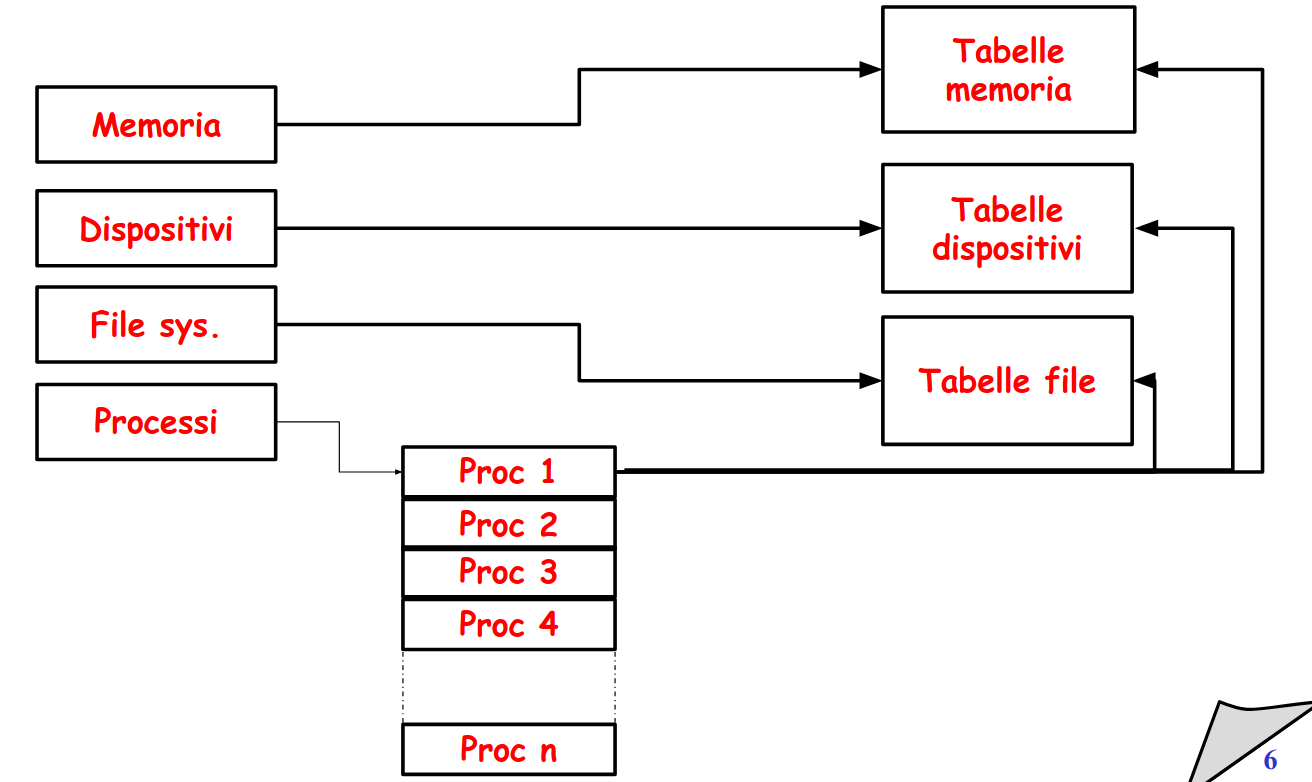
\includegraphics[width=0.7\linewidth]{Images/Screenshot 2024-12-18 at 15-07-44 so-02.1-scheduling - so-02.1-scheduling.pdf.png}
    \caption{Tabelle per la gestione}
\end{figure}

\subsection{Descrittori dei processi}
\paragraph{Qual é la manifestazione fisica di un processo?}

\begin{enumerate}
    \item il codice da eseguire (segmento codice)
    \item i dati su cui operare (segmenti dati)
    \item uno stack di lavoro per la gestione di chiamate di funzione, passaggio di
parametri e variabili locali
    \item un insieme di attributi contenenti tutte le informazioni necessarie per la gestione del processo stesso

\end{enumerate}

Questo insieme di attributi prende il nome di descrittore del processo (process control block, PCB).

\begin{figure} [h]
    \centering
    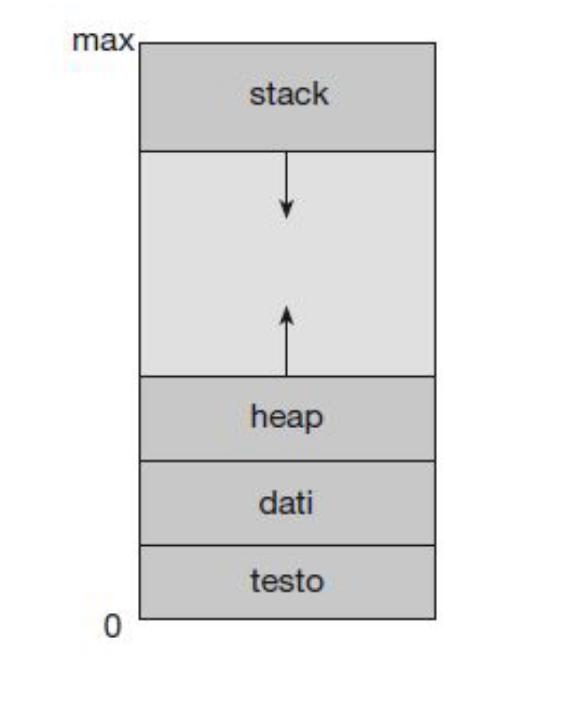
\includegraphics[width=0.3\linewidth]{Images/Screenshot 2024-12-18 at 18-22-19 so-02.1-scheduling - so-02.1-scheduling.pdf.png}
    \caption{Processo in memoria}
\end{figure}
\newpage
\paragraph{Tabella per la gestione dei processi:} contiene i descrittori dei processi, ogni processo ha un descrittore associato.
E' possibile suddividere le informazioni contenute nel descrittore in tre aree:
\begin{itemize}
    \item informazioni di identificazione di processo
    \item informazioni di stato del processo
    \item informazioni di controllo del processo
\end{itemize}

\subsubsection{Informazioni di identificazione di un processo}
L'identificatore di processo (process id, o pid), può essere semplicemente un indice all'interno di una tabella di processi.
Può essere un numero progressivo; in caso, è necessario
un mapping tra pid e posizione del relativo descrittore, molte altre tabelle del s.o. utilizzano il process id per identificare un elemento della tabella dei processi.

Possono essere identificatori di altri processi logicamente collegati al processo. \textit{Ad esempio, pid del processo padre}

Id dell'utente che ha richiesto l'esecuzione del processo

\subsubsection{Informazioni di stato del processo}
Come registri generali del processore o registri speciali, come il program counter e i registri di stato.

\subsubsection{Informazioni di controllo del processo}
\textbf{Informazioni di scheduling:} stato del processo (in esecuzione, pronto, in attesa), informazioni particolari necessarie dal particolare algoritmo di scheduling utilizzato, identificatore dell'evento per cui il processo è in attesa.
\newline
\textbf{Informazioni di gestione della memoria:} valori dei registri base e limite dei segmenti utilizzati, puntatori alle tabelle delle pagine, etc.
\newline
\textbf{Informazioni di accounting:} tempo di esecuzione del processo, tempo trascorso dall'attivazione di un processo.
\newline
\textbf{Informazioni relative alle risorse:} risorse controllate dal processo, come file aperti, device allocati al processo.
\newline
\textbf{Informazioni per interprocess communication (IPC):} stato di segnali, semafori, etc.

\subsection{Scheduler}
Lo scheduler è la componente più importante del kernel, gestisce l'avvicendamento dei processi decidendo quale processo deve essere in esecuzione ad ogni istante, interviene quando viene richiesta un'operazione di I/O e quando un'operazione di I/O termina, ma anche periodicamente.

\begin{figure} [h]
    \centering
    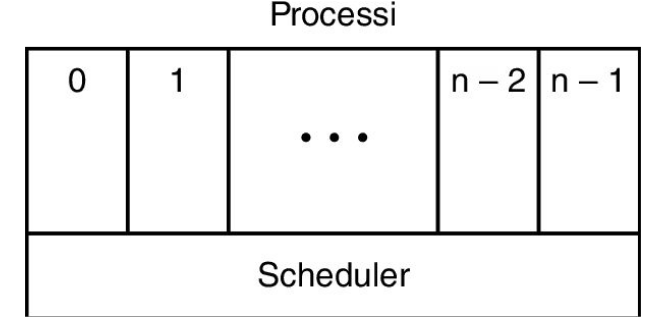
\includegraphics[width=0.35\linewidth]{Images/Screenshot 2024-12-18 at 18-47-56 so-02.1-scheduling - so-02.1-scheduling.pdf.png}
\end{figure}
\textbf{Schedule:} è la sequenza temporale di assegnazioni delle risorse da gestire ai richiedenti.

\textbf{Scheduling:} è l'azione di calcolare uno schedule.

\textbf{Scheduler:} è la componente software che calcola lo schedule.

\subsection{Mode switching e Context switching}
Tutte le volte che avviene un interrupt (software o hardware) il
processore è soggetto ad un \textbf{mode switching} (modalità utente → modalità supervisore)
Durante la gestione dell'interrupt vengono intraprese le opportune azioni per gestire l'evento. Viene chiamato lo scheduler: se lo scheduler decide di eseguire un altro processo, il sistema è soggetto ad un \textbf{context switching}.

Durante un context switching, lo stato del processo attuale viene salvato nel PCB corrispondente mentre lo stato del processo selezionato per l'esecuzione viene caricato dal PCB
nel processore.
\begin{figure} [h]
    \centering
    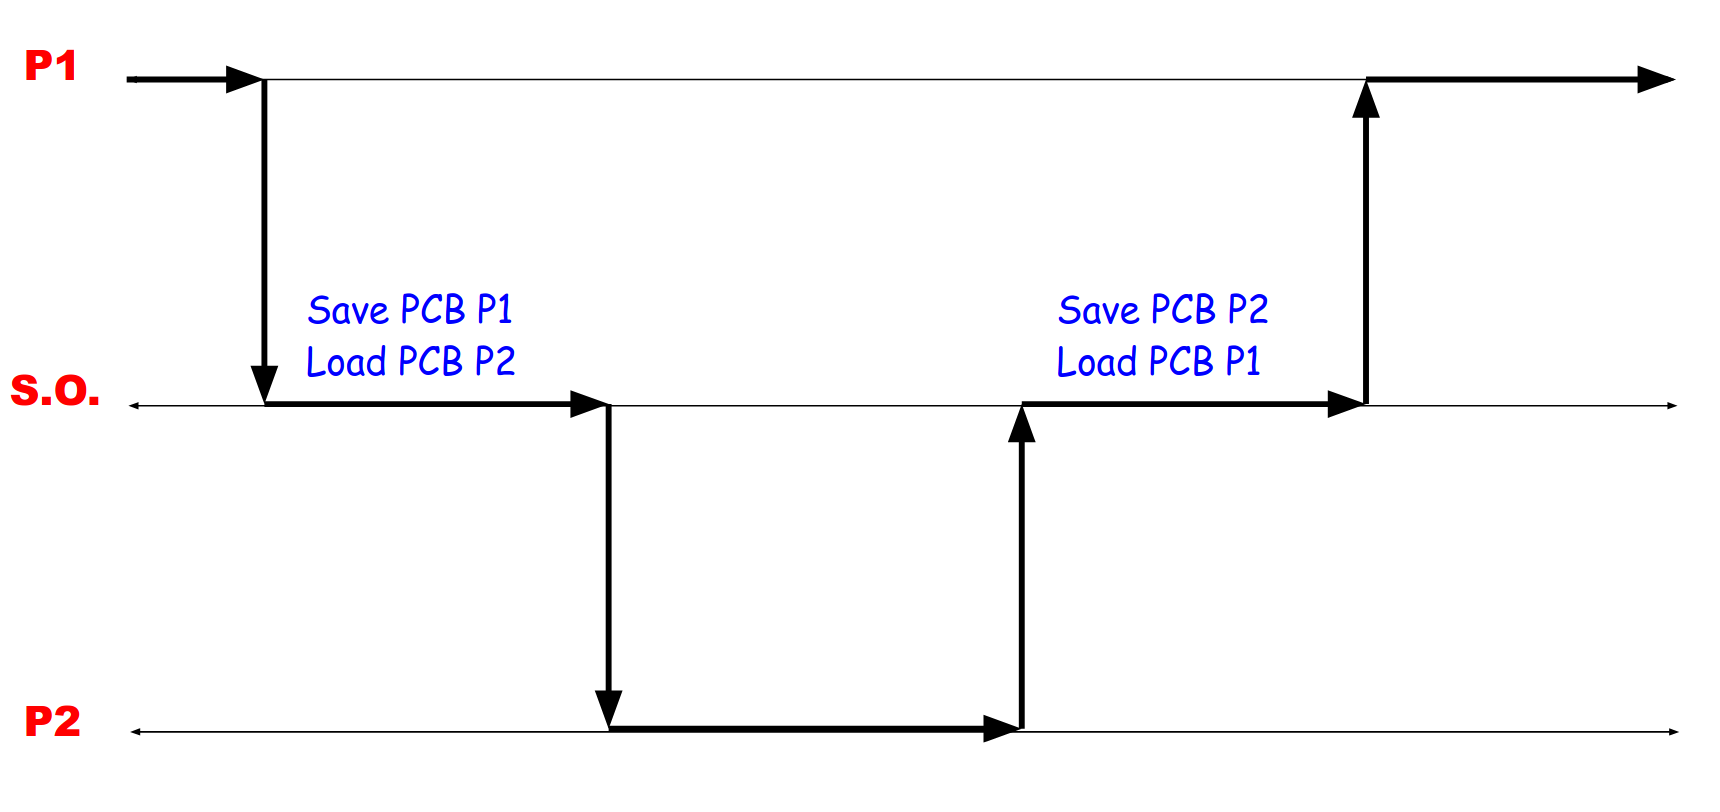
\includegraphics[width=0.6\linewidth]{Images/Screenshot 2024-12-18 at 18-58-00 so-02.1-scheduling - so-02.1-scheduling.pdf.png}
    \caption{Funzionamento del context switch}
\end{figure}




\subsection{Processi e Thread}

\subsubsection{Vita di un processo}
Gli stati di un processo possono essere:
\newline

\textbf{Running:} il processo è in esecuzione.

\textbf{Waiting:} il processo è in attesa di qualche evento esterno (e.g., completamento.
operazione di I/O); non può essere eseguito.

\textbf{Ready:} il processo può essere eseguito, ma attualmente il processore è impegnato in altre attività.

\begin{figure} [h]
    \centering
    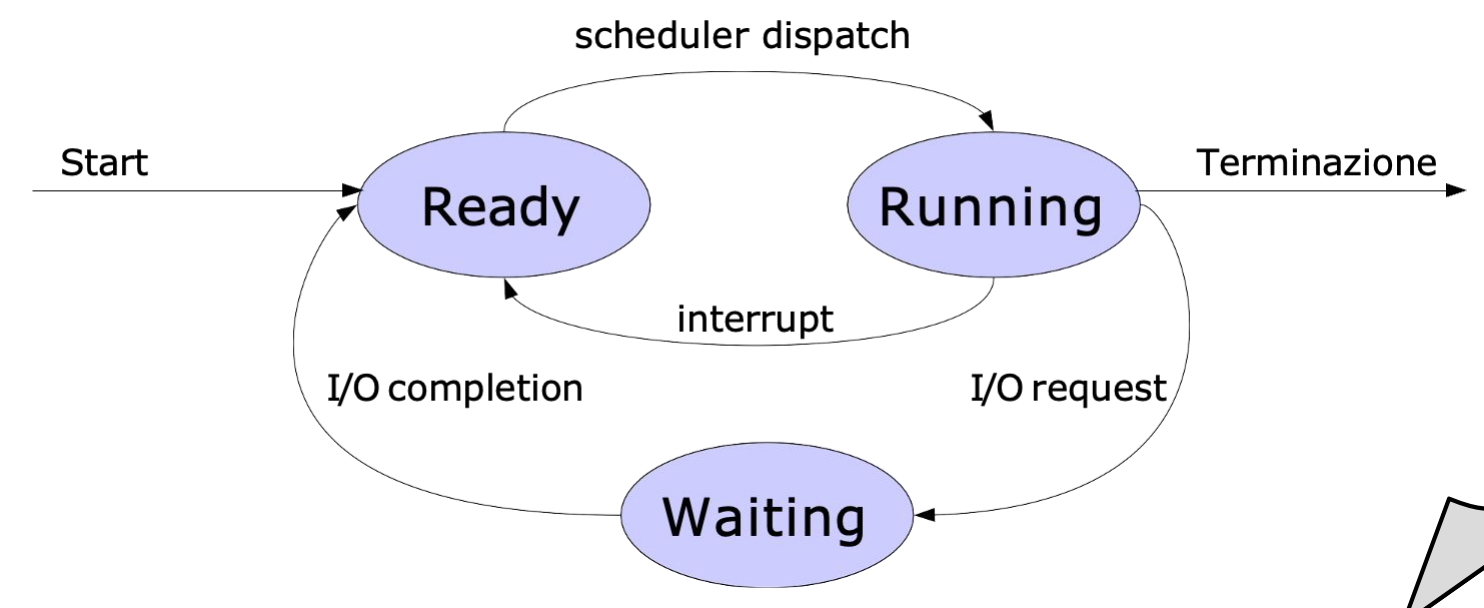
\includegraphics[width=0.6\linewidth]{Images/Screenshot 2024-12-23 at 12-34-55 so-02.1-scheduling - so-02.1-scheduling.pdf.png}
    \caption{Stati dei processi}
\end{figure}

Tutte le volte che un processo entra nel sistema, viene posto in una delle code gestite dallo scheduler.

\begin{figure} [h]
    \centering
    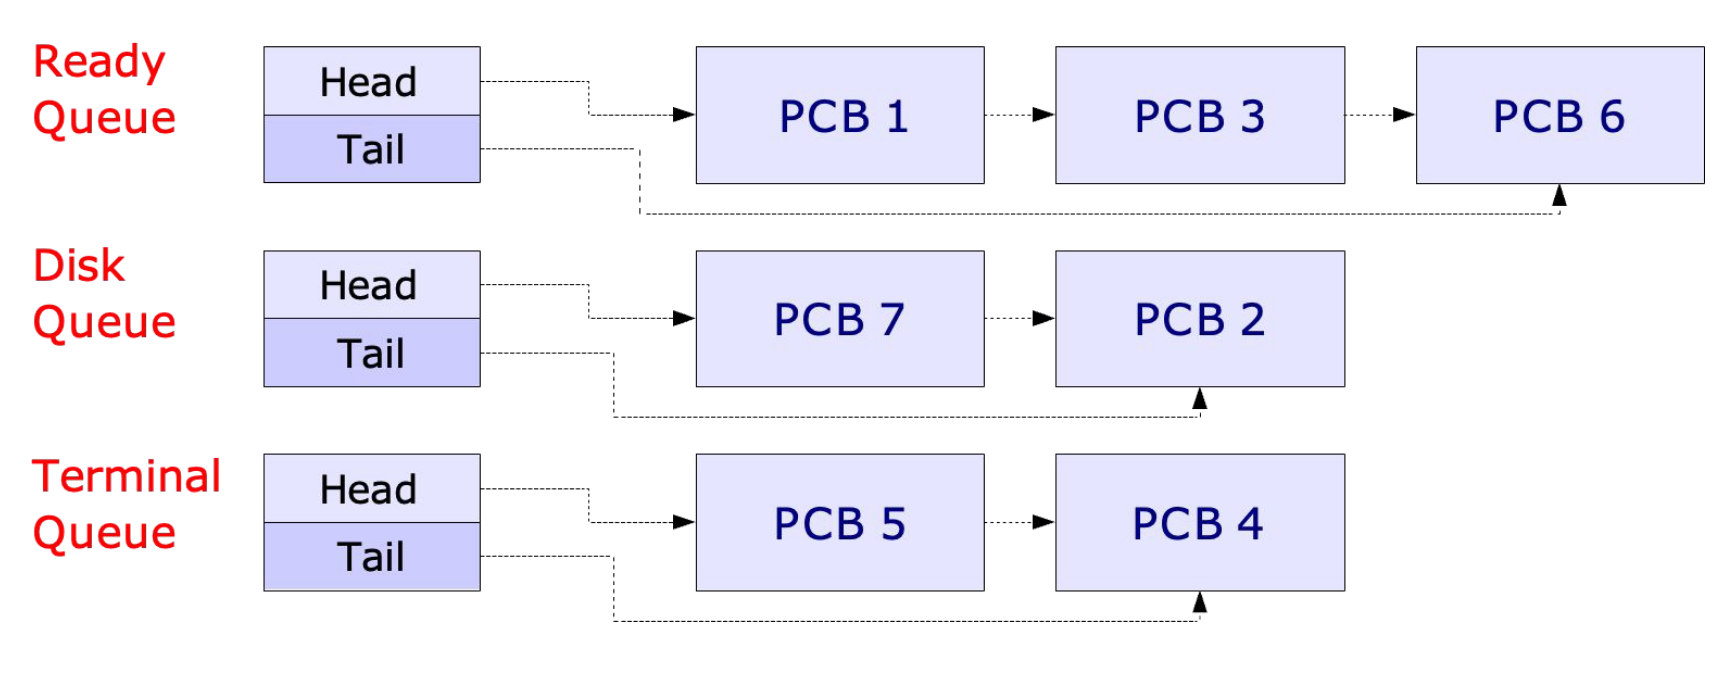
\includegraphics[width=0.6\linewidth]{Images/Screenshot 2024-12-23 at 12-37-44 so-02.1-scheduling - so-02.1-scheduling.pdf.png}
    \caption{Le code gestite dallo scheduler}
\end{figure}

\subsubsection{Gerarchia di processi}
Nella maggior parte dei sistemi operativi i processi sono organizzati in forma gerarchica.

Quando un processo crea un nuovo processo, il processo creante viene
detto padre e il creato figlio
si viene così a creare un albero di processi.

Le motivazioni sono la semplificazione del procedimento di creazione di processi, non occorre specificare esplicitamente tutti i parametri e le caratteristiche e ciò che non viene specificato, viene ereditato dal padre.

\begin{figure}[h]
    \centering
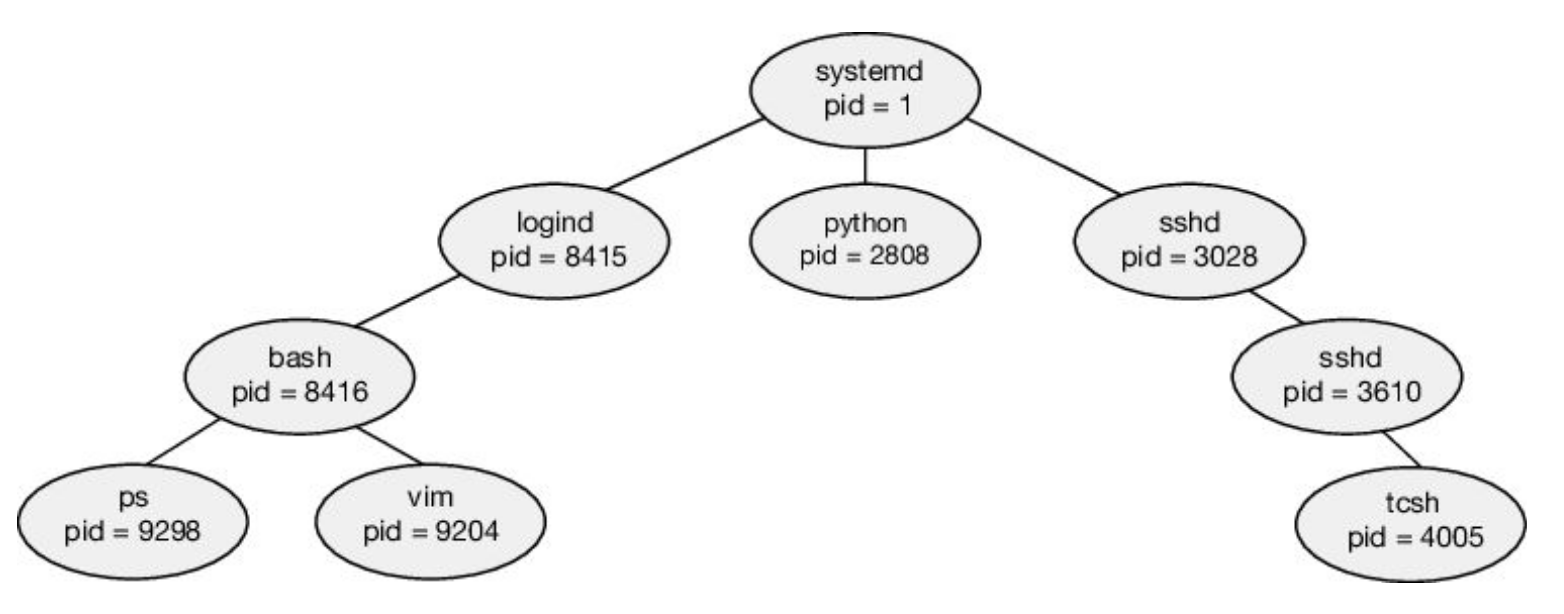
\includegraphics[width=0.6\linewidth]{Images/Screenshot 2024-12-23 at 12-42-11 so-02.1-scheduling - so-02.1-scheduling.pdf.png}
    \caption{Albero dei processi di un sistema Linux}
\end{figure}

\subsubsection{Threads}
\paragraph{}
La nozione di processo discussa in precedenza assume che ogni
processo abbia una singola “linea di controllo”. Per ogni processo, viene eseguite una singola sequenza di istruzioni, un singolo processo non può eseguire due differenti attività
contemporaneamente.

\textit{Esempi: scaricamento di due differenti pagine in un web browser, inserimento di nuovo testo in un wordprocessor mentre viene eseguito il correttore ortografico}

\paragraph{}
Tutti i sistemi operativi moderni supportano l’esistenza di processi \textbf{multithreaded}. In un processo multithreaded esistono molte “linee di controllo”, ognuna
delle quali può eseguire un diverso insieme di istruzioni.

\textit{Esempi: Associando un thread ad ogni finestra aperta in un web browser, è possibile scaricare i dati in modo indipendente.
}

\paragraph{Cos'è un thread?}
Un thread è l’unità base di utilizzazione della CPU.
Ogni thread possiede la propria copia dello stato del processore, il proprio program counter e uno stack separato.
I thread appartenenti allo stesso processo condividono: codice, dati e risorse di I/O.

\begin{figure} [h]
    \centering
    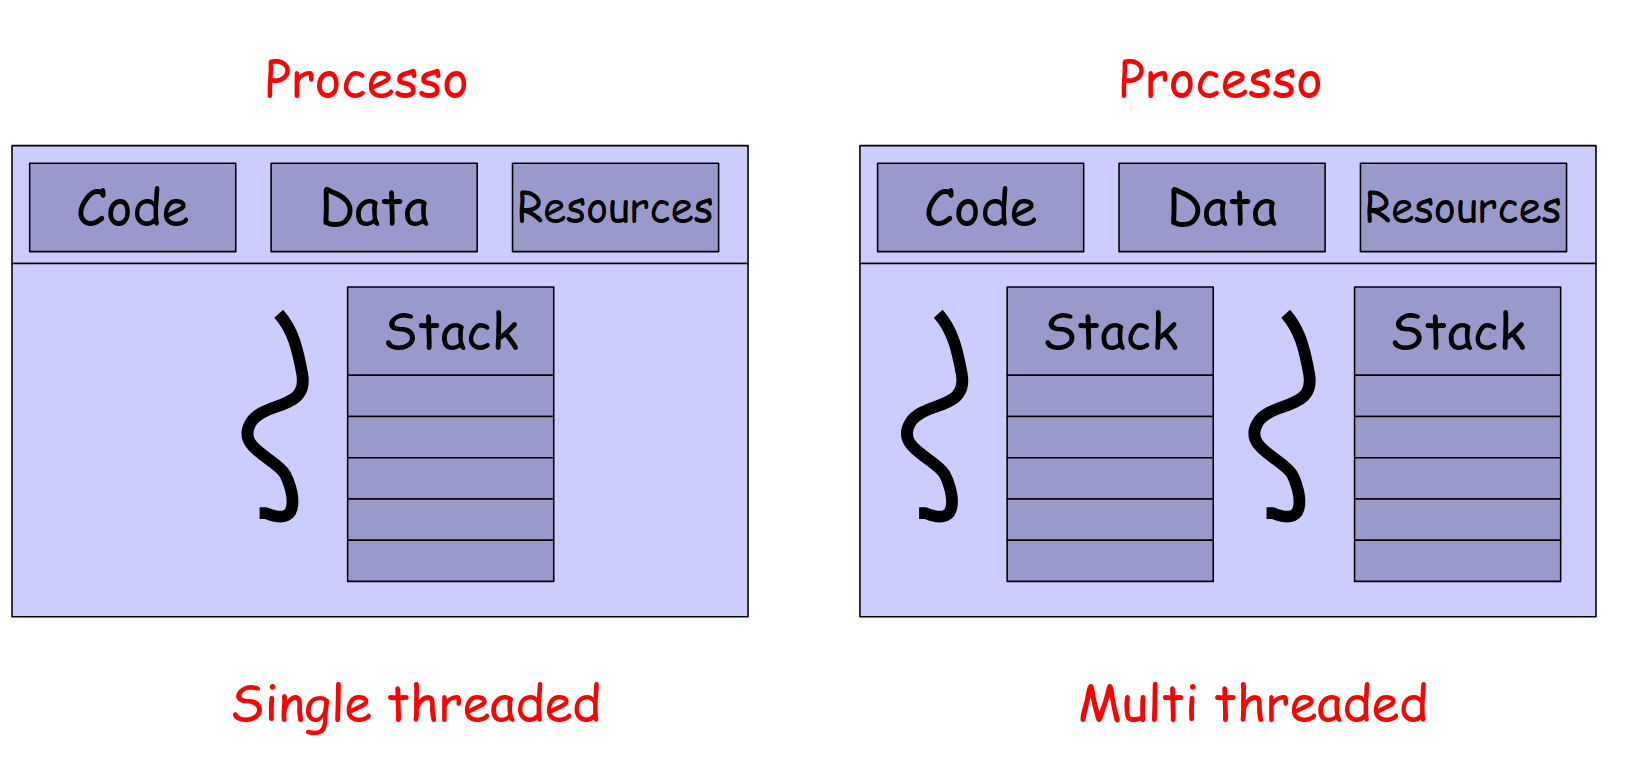
\includegraphics[width=0.6\linewidth]{Images/Screenshot 2024-12-23 at 12-51-01 so-02.1-scheduling - so-02.1-scheduling.pdf.png}
    \caption{Singlethreaded e multithreaded}
\end{figure}

\paragraph{Benefici dei thread}
La condivisione di risorse: i thread condividono lo spazio di memoria e le risorse allocate degli altri thread dello stesso processo. Condividere informazioni tra thread logicamente correlati rende più semplice l’implementazione di certe applicazioni.

\textit{Esempio: web browser: condivisione dei parametri di configurazione fra i vari thread.}
\newline

Economia: allocare memoria e risorse per creare nuovi processi è costoso, fare context switching fra diversi processi non è ottimale. 
Mentre gestire i thread è in generale più economico, creare thread all’interno di un processo permette di fare context switching fra thread che è meno costoso.

\textit{Esempio: creare un thread in Solaris richiede 1/30 del tempo richiesto per creare un nuovo processo.}

\textbf{Thread = processi "lightweight"}
Utilizzare i thread al posto dei processi rende l’implementazione più efficiente. In ogni caso, abbiamo bisogno di processi distinti per applicazioni differenti.

\subsection{Multithreading}

Un sistema operativo può implementare i thread in due modi:
\begin{itemize}
    \item User thread
    \item Kernel thread
\end{itemize}

\subsubsection{User thread}
Gli user thread vengono supportati sopra il kernel e vengono
implementati da una \textbf{thread library} a livello utente. La thread library fornisce supporto per la creazione, lo scheduling e la gestione dei thread senza alcun intervento del kernel.

\textbf{Vantaggi:} l’implementazione risultante è molto efficiente.
\newline

\textbf{Svantaggi:} Se il kernel è single-threaded, qualsiasi user thread che effettua una chiamata di sistema bloccante (che si pone in attesa di I/O) causa il blocco dell’intero processo.

\subsubsection{Kernel thread}
I kernel thread vengono supportati direttamente dal sistema
operativo. La creazione, lo scheduling e la gestione dei thread sono implementati a livello kernel.

\textbf{Vantaggi:} poichè è il kernel a gestire lo scheduling dei thread, se un thread esegue una operazione di I/O, il kernel può selezionare un altro thread in attesa di essere eseguito.
\newline

\textbf{Svantaggi:} l’implementazione risultante è più lenta, perché richiede un passaggio da
livello utente a livello supervisore

\subsubsection{Modelli di multithreading}
Molti sistemi supportano sia kernel thread che user thread.
Si vengono così a creare tre differenti modelli di multithreading:

\begin{itemize}
    \item Many-to-One
    \item One-to-One
    \item Many-to-Many
\end{itemize}

\paragraph{Many-to-One}
Un certo numero di user thread vengono mappati su un solo
kernel thread. Modello generalmente adottato da s.o. che non supportano kernel thread multipli.

\begin{figure} [h]
    \centering
    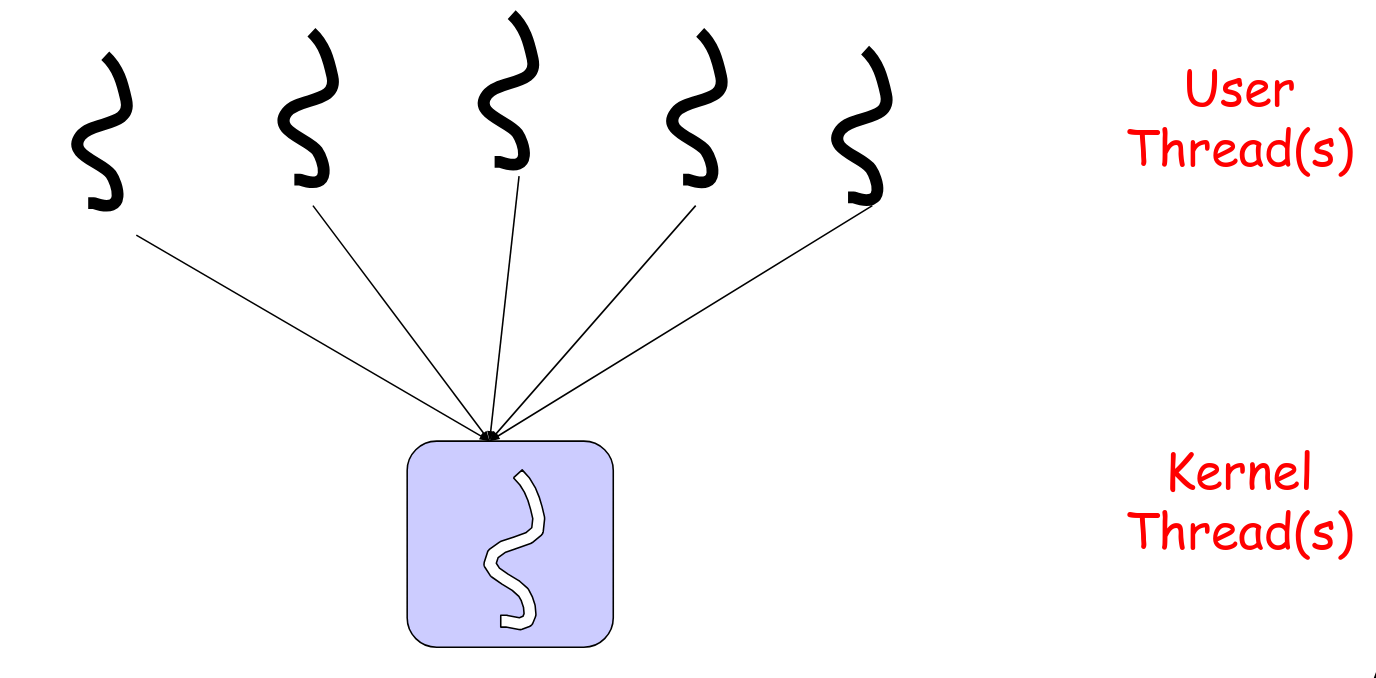
\includegraphics[width=0.5\linewidth]{Images/Screenshot 2024-12-23 at 13-14-46 so-02.1-scheduling - so-02.1-scheduling.pdf.png}
\end{figure}

\paragraph{One-to-One}
Ogni user thread viene mappato su un kernel thread. Può creare problemi di scalabilità per il kernel.

\begin{figure} [h]
    \centering
    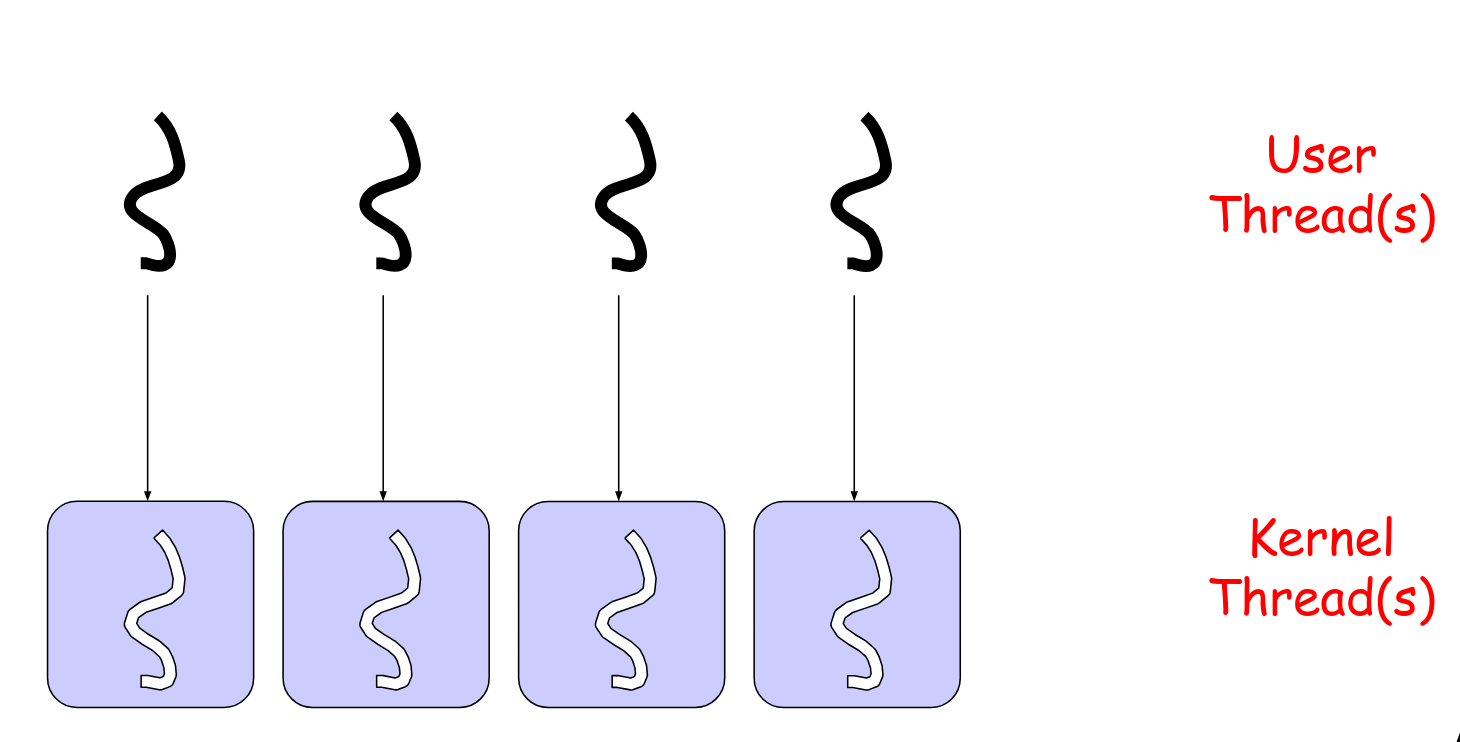
\includegraphics[width=0.5\linewidth]{Images/Screenshot 2024-12-23 at 13-16-34 so-02.1-scheduling - so-02.1-scheduling.pdf.png}
\end{figure}
\newpage
\paragraph{Many-to-Many}
Riassume i benefici di entrambe le architetture. Supportato da Solaris, IRIX, Digital Unix.

\begin{figure} [h]
    \centering
    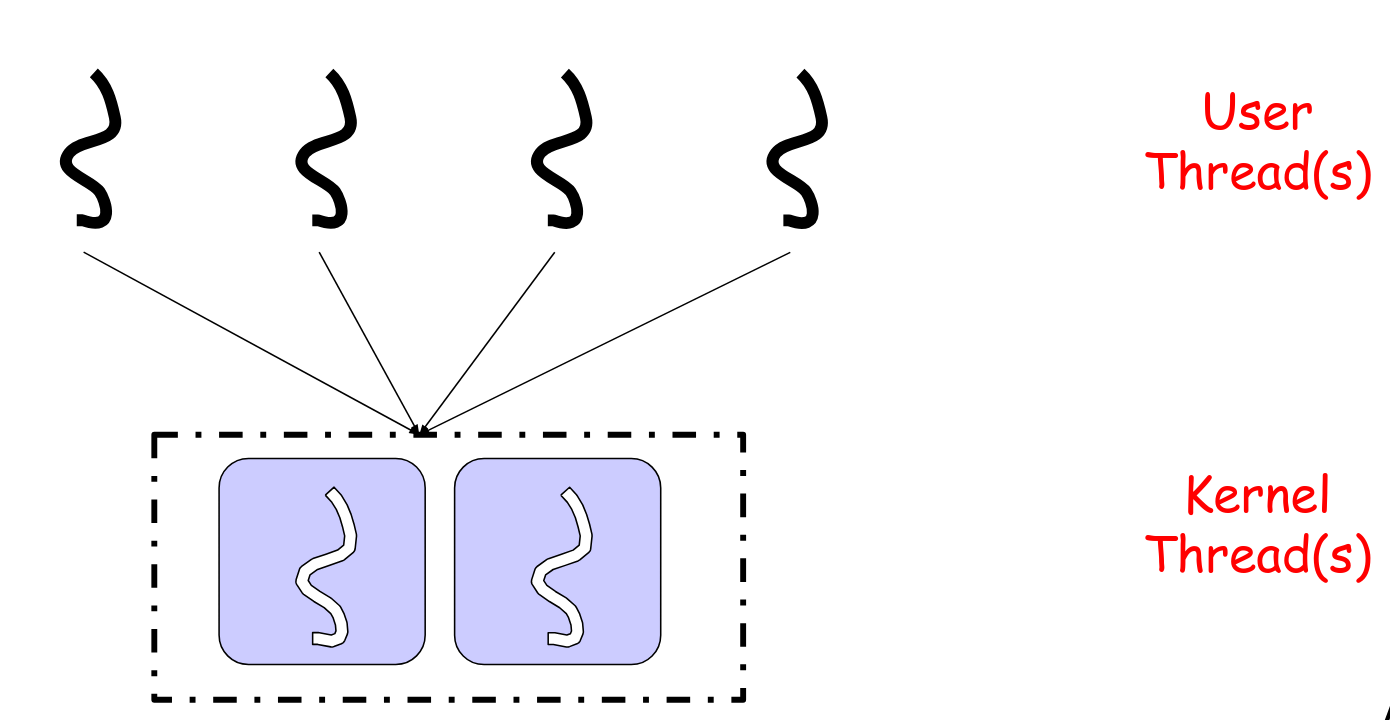
\includegraphics[width=0.5\linewidth]{Images/Screenshot 2024-12-23 at 13-17-03 so-02.1-scheduling - so-02.1-scheduling.pdf.png}
\end{figure}

\section{Schedule}

\subsection{Rappresentazione degli schedule}
Per rappresentare uno schedule si usano i diagrammi di Gantt
\begin{figure} [h]
    \centering
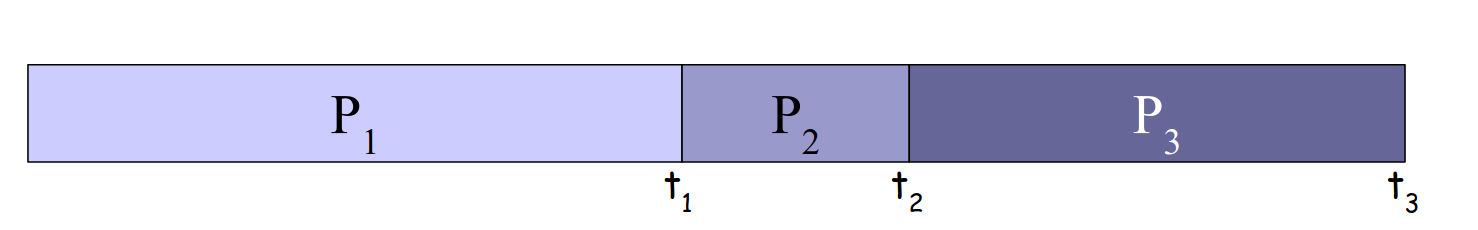
\includegraphics[width=0.5\linewidth]{Images/Screenshot 2024-12-23 at 13-32-35 so-02.1-scheduling - so-02.1-scheduling.pdf.png}
    \caption{In questo esempio, la risorsa (es. CPU) viene utilizzata dal processo $P_1$ dal tempo 0 a $t_1$, viene quindi assegnata a $P_2$ fino al tempo $t_2$ e quindi a $P_3$ fino al tempo $t_3$.}
\end{figure}
\newline

Nel caso si debba rappresentare lo schedule di più risorse (\textit{e.g., un sistema multiprocessore)} il diagramma di Gantt risulta composto da più righe parallele.

\begin{figure} [h]
    \centering
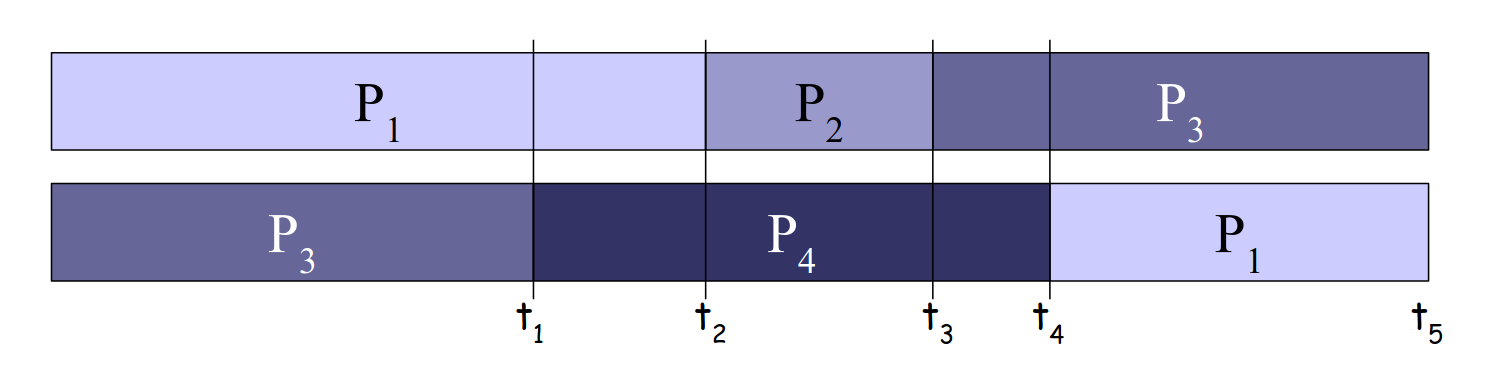
\includegraphics[width=0.5\linewidth]{Images/Screenshot 2024-12-23 at 13-37-03 so-02.1-scheduling - so-02.1-scheduling.pdf.png}
    \caption{Diagramma di Gantt multi-risorsa}
\end{figure}

\subsubsection{Tipi di scheduler}
Eventi che possono causare un context switch:
\begin{enumerate}
    \item quando un processo passa da stato running a stato waiting(system call bloccante, operazione di I/O).
    \item quando un processo passa dallo stato running allo stato ready (a causa di un interrupt).
    \item quando un processo passa dallo stato waiting allo stato ready.
    \item quando un processo termina.
\end{enumerate}

\textit{(Nota: nelle condizioni 1 e 4, l'unica scelta possibile è quella di selezionare un altro processo per l'esecuzione. Nelle condizioni 2 e 3, è possibile continuare ad eseguire il processo corrente)}
\newline

Uno scheduler si dice \textbf{non-preemptive} (o cooperativo) se i context switch avvengono solo nelle condizioni 1 e 4. In altre parole: il controllo della risorsa viene trasferito solo se l'assegnatario attuale lo cede volontariamente.
Vantaggi: non richiede alcuni meccanismi hardware come ad esempio timer programmabili.

Uno scheduler si dice \textbf{preemptive} (tutti gli scheduler moderni) se i context switch possono avvenire in ogni condizione. In altre parole: è possibile che il controllo della risorsa venga tolto all'assegnatario attuale a causa di un evento. 
Vantaggi: permette di utilizzare al meglio le risorse.
\newpage
\subsubsection{Criteri di scelta di uno scheduler}
\begin{itemize}
    \item \textbf{Utilizzo della risorsa (CPU):} lq percentuale di tempo in cui la CPU è occupata ad eseguire processi deve essere massimizzato.
    \item \textbf{Throughput:} numero di processi completati per unità di tempo. Dipende dalla lunghezza dei processi, deve essere massimizzato.
    \item \textbf{Tempo di turnaround:} tempo che intercorre dalla sottomissione di un processo alla sua terminazione, deve essere minimizzato.
    \item \textbf{Tempo di attesa:} il tempo trascorso da un processo nella coda ready, deve essere minimizzato.
    \item \textbf{Tempo di risposta:} il tempo che intercorre fra la sottomissione di un processo e il tempo di prima risposta. Particolarmente significativo nei programmi interattivi, deve essere minimizzato.
\end{itemize}

\subsubsection{Caratteristiche dei processi}
Durante l'esecuzione di un processo si alternano periodi di attività svolte dalla CPU (\textbf{CPU burst}) e periodi di attività di I/O (\textbf{I/O burst}).

I processi caratterizzati da CPU burst molto
lunghi si dicono \textbf{CPU bound}, mentre quelli caratterizzati da I/O burst molto lunghi si dicono \textbf{I/O bound}.

\begin{figure} [h]
    \centering
    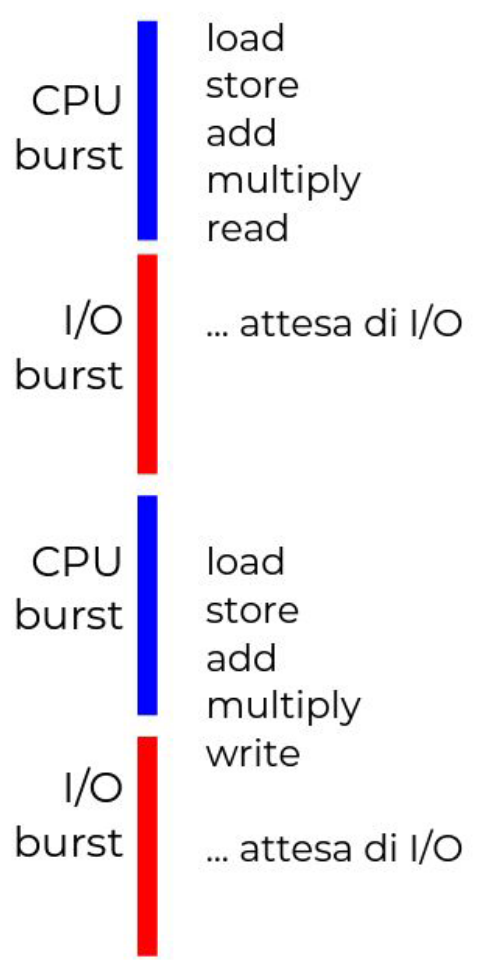
\includegraphics[width=0.2\linewidth]{Images/Screenshot 2024-12-23 at 14-20-04 so-02.1-scheduling - so-02.1-scheduling.pdf.png}
\end{figure}

\section{Algoritmi di scheduling}
Gli algoritmi di scheduling che vedremo sono:
\begin{itemize}
    \item First Come, First Served
    \item Shortest-Job First
    \begin{itemize}
        \item Shortest-Next-CPU-Burst First
        \item Shortest-Remaining-Time-First
    \end{itemize}
    \item Round-Robin
    \item Scheduling a priorità
    \item Scheduling a classi di priorità
    \item Scheduling multilivello
\end{itemize}

\subsection{First Come, First Served (FCFS)}
\paragraph{Algoritmo:} il processo che arriva per primo, viene servito per primo, politica senza preemption.

Supponiamo di avere: un processo CPU bound, un certo numero di processi I/O bound. 
I processi I/O bound si "mettono in coda" dietro al processo CPU bound, e in alcuni casi la ready queue si puo svuotare (convoy effect).

\begin{figure} [h]
    \centering
    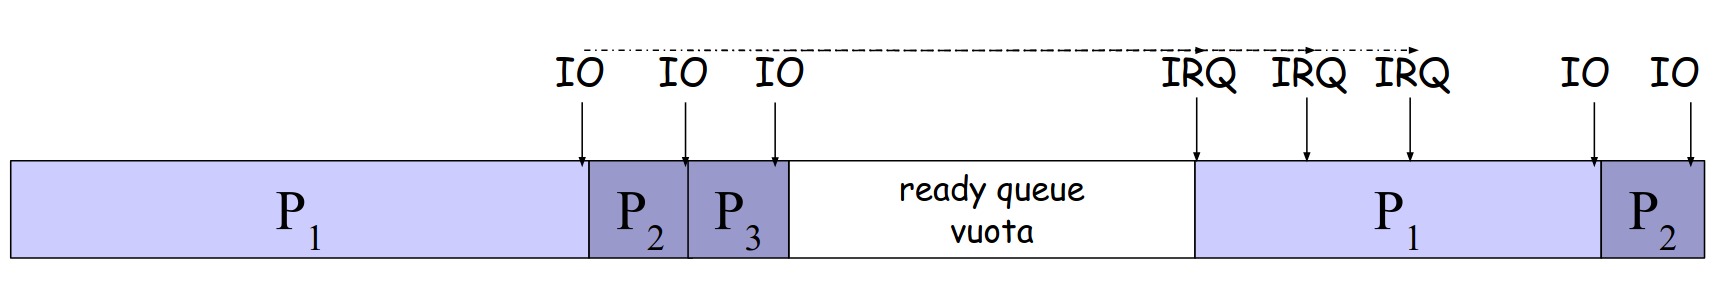
\includegraphics[width=0.5\linewidth]{Images/Screenshot 2024-12-23 at 14-30-35 so-02.1-scheduling - so-02.1-scheduling.pdf.png}
\end{figure}

\paragraph{Implementazione:} semplice, tramite una coda (politica FIFO)
\paragraph{Problemi:} elevati tempi medi di attesa e di turnaround, processi CPU bound ritardano i processi I/O bound.

\textit{Esempio:}
\begin{figure} [h]
    \centering
    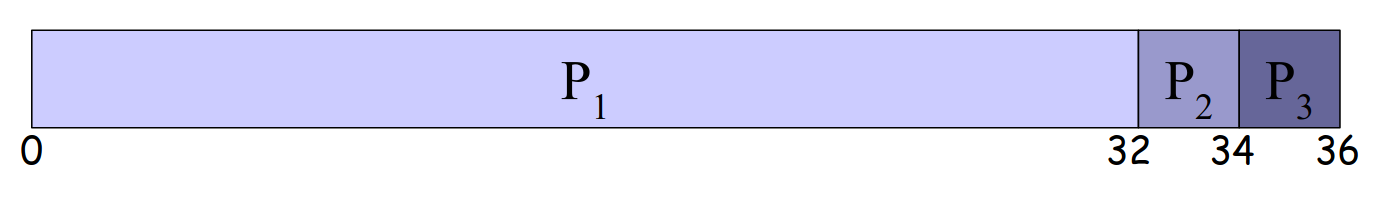
\includegraphics[width=0.5\linewidth]{Images/Screenshot 2024-12-23 at 14-25-16 so-02.1-scheduling - so-02.1-scheduling.pdf.png}
    \caption{Ordine di arrivo: $P_1$, $P_2$, $P_3$
\newline
Lunghezza dei CPU-burst in ms: 32, 2, 2
\newline
Tempo medio di turnaround: (32+34+36)/3 = 34 ms
\newline
Tempo medio di attesa: (0+32+34)/3 = 22 ms}
\end{figure}

\subsection{Shortest Job First (SJF)}
\paragraph{Algoritmo:} la CPU viene assegnata al processo ready che ha la minima durata del CPU burst successivo, politica senza preemption.

\paragraph{Problemi:} è ottimale rispetto al tempo di attesa, in quanto è possibile dimostrare che produce il minor tempo di attesa possibile, ma è impossibile da implementare in pratica! E' possibile solo fornire delle approssimazioni.

Negli scheduler long-term possiamo chiedere a chi sottomette un job di predire la durata del job.
Negli scheduler short-term non possiamo conoscere la lunghezza del prossimo CPU burst ma conosciamo la lunghezza di quelli precedenti.

\textit{Esempio:}
\begin{figure} [h]
    \centering
    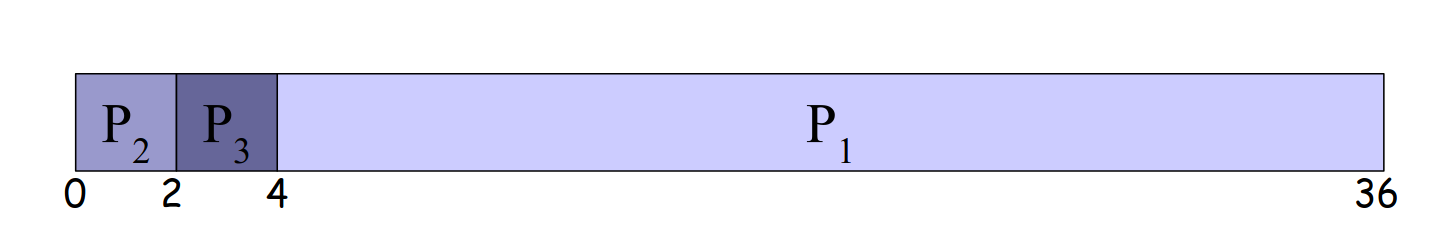
\includegraphics[width=0.5\linewidth]{Images/Screenshot 2024-12-23 at 14-33-56 so-02.1-scheduling - so-02.1-scheduling.pdf.png}
    \caption{Tempo medio di turnaround: (0+2+4+36)/3 = 7 ms
\newline
Tempo medio di attesa: (0+2+4)/3 = 2 ms}
\end{figure}


\paragraph{Calcolo approssimato della durata del CPU burst}
basata su media esponenziale dei CPU burst precedenti
sia $t_n$ il tempo dell'n-esimo CPU burst e $T_n$ la corrispondente previsione;
$T_{n+1}$ può essere calcolato come segue:
$T_{n+1} = \alpha t_{n} + (1-\alpha) T_{n}$

\paragraph{Media esponenziale}
svolgendo la formula di ricorrenza, si ottiene:
\newline

$T_{n+1} = \sum_{j=0}^n \alpha(1-\alpha)^j t_{n-j} + (1-\alpha)^{n+1} T_0$
\newline

\textbf{Spiegazione:} 
\begin{itemize}
    \item [-] $t_n$ rappresenta la storia recente.
    \item [-] $T_n$ rappresenta la storia passata.
    \item [-] $\alpha$ rappresenta il peso relativo di storia passata e recente.
\end{itemize}
\textit{(Nota: SJF può essere soggetto a starvation)}

\paragraph{}
Shortest Job First "approssimato" esiste in due versioni:
\newline
\textbf{Non preemptive: Shortest-Next-CPU-Burst First} 
Il processo corrente esegue fino al completamento del suo CPU burst.
\newline
\textbf{Preemptive: Shortest-Remaining-Time First} 
Il processo corrente può essere messo nella coda ready, se arriva un processo con un CPU burst più breve di quanto rimane da eseguire al processo corrente.

\subsection{Round-Robin}
E' basato sul concetto di \textbf{quanto di tempo} (o time slice). Un processo non può rimanere in esecuzione per un tempo superiore alla durata del quanto di tempo.

La durata del quanto di tempo è un parametro critico del sistema, se il quanto di tempo è breve, il sistema è meno efficiente perché deve cambiare il processo attivo più spesso.

Se il quanto è lungo, in presenza di numerosi processi pronti ci sono lunghi periodi di inattività di ogni singolo processo. (In sistemi interattivi, questo può essere fastidioso per gli   utenti).


\paragraph{Implementazione:} l'insieme dei processi pronti è organizzato come una coda.
Due possibilità:
\begin{itemize}
    \item un processo può lasciare il processore volontariamente, in seguito ad un'operazione di I/O.
    \item un processo può esaurire il suo quanto di tempo senza completare il suo CPU burst, nel qual caso viene aggiunto in fondo alla coda dei processi pronti.
\end{itemize}

In entrambi i casi, il prossimo processo da eseguire è il primo della coda dei processi pronti.
\newline

Nell'implementazione è necessario che l'hardware fornisca un timer (\textbf{interval timer}) che agisca come "sveglia" del processore.

Il timer è un dispositivo che, attivato con un preciso valore di tempo, è in grado di fornire un interrupt allo scadere del tempo prefissato, viene interfacciato come se fosse un'unita di I/O.
\newline

\textit{Esempio:}

\begin{figure} [h]
    \centering
    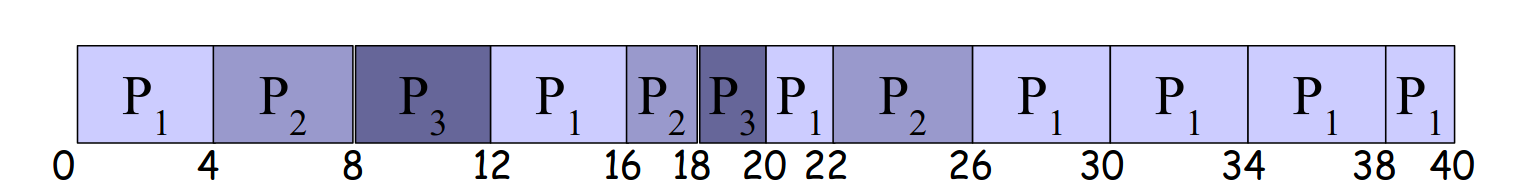
\includegraphics[width=0.5\linewidth]{Images/Screenshot 2024-12-23 at 15-06-19 so-02.1-scheduling - so-02.1-scheduling.pdf.png}
    \caption{}
\end{figure}

Tre processi: $P_1$, $P_2$, $P_3$
\newline
Lunghezza dei CPU-burst in ms ($P_1$: 10+14; $P_2$: 6+4; $P_3$: 6)
\newline
Lunghezza del quanto di tempo: 4
\newline
Tempo medio di turnaround (40+26+20)/3 = 28.66 ms
\newline
Tempo medio di attesa: (16+16+14)/3 = 15.33 ms
\newline
Tempo medio di risposta: 4 ms

\subsection{Scheduling a priorità}

Il round-robin fornisce le stesse possibilità di esecuzione a tutti i processi. 
Ma i processi non sono tutti uguali, infatti usando round-robin puro la visualizzazione dei un video MPEG potrebbe essere ritardata da un processo che sta per esempio smistando la posta, la lettera può aspettare mezzo secondo, il frame video no!

\textit{Vediamo quindi come impostare un round-robin con delle priorità...}

\paragraph{Descrizione:} a ogni processo è associata una specifica priorità, lo scheduler sceglie il processo pronto con priorità più alta.
\newline

Le priorità possono essere: 
\begin{itemize}
    \item \textbf{Definite dal sistema operativo:} vengono utilizzate una o più variabili per calcolare la priorità di un processo.
    \textit{Esempio: SJF è un sistema basato su priorità}
    \item \textbf{Definite esternamente:} le priorità non vengono definite dal sistema operativo, ma vengono imposte dal livello utente.
\end{itemize}

\begin{figure} [h]
    \centering
    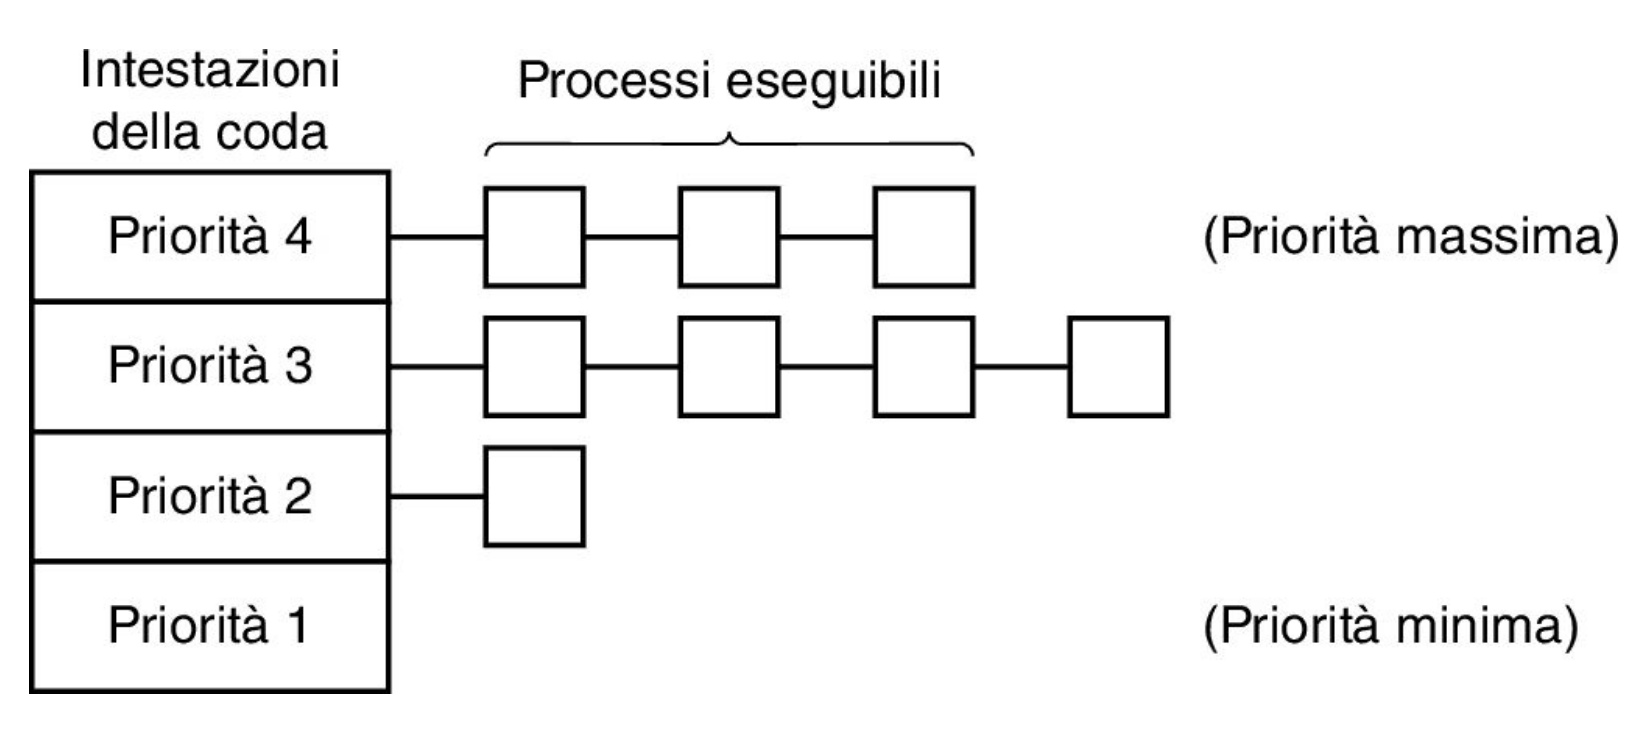
\includegraphics[width=0.6\linewidth]{Images/Screenshot 2024-12-23 at 17-14-31 so-02.1-scheduling - so-02.1-scheduling.pdf.png}
    \label{fig:enter-label}
\end{figure}

\subsubsection{Tecniche di assegnazione delle priorità}

\paragraph{Priorità statica:} la priorità non cambia durante la vita di un processo. Un problema di questa tecnica è che i processi a bassa priorità possono essere posti in starvation da processi ad alta priorità.

\paragraph{Priorità dinamica:} la priorità può variare durante la vita di un processo, è possibile utilizzare metodologie di priorità dinamica per evitare starvation

\paragraph{Priorità basata su aging:} tecnica che consiste nell'incrementare gradualmente la priorità dei processi
in attesa, posto che il range di variazione delle priorità sia limitato, nessun processo rimarrà in attesa per un tempo indefinito perché prima o poi raggiungerà la priorità massima.


\subsection{Scheduling a classi di priorità}

\paragraph{Descrizione:} è possibile creare diverse classi di processi con caratteristiche simili e assegnare ad ogni classe specifiche priorità. La coda ready viene quindi scomposta in molteplici "sottocode", una per ogni classe di processi.

\paragraph{Algoritmo:} uno scheduler a classi di priorità seleziona il processo da eseguire fra quelli pronti della classe a priorità massima che contiene processi.

\subsection{Scheduling multilivello}
\paragraph{Descrizione:} all'interno di ogni classe di processi, è possibile utilizzare una politica specifica adatta alle caratteristiche della classe. 

Uno scheduler multilivello cerca prima la classe di priorità massima che ha almeno un processo ready, sceglie poi il processo da porre in stato running coerentemente con la politica specifica della classe.
\newline

\textbf{Quattro classi di processi (priorità decrescente):}

\begin{itemize}
    \item processi server \textit{(priorità statica)}
    \item processi utente interattivi \textit{(round-robin)}
    \item altri processi utente \textit{(FIFO)}
    \item processo vuoto \textit{(FIFO banale)}
\end{itemize}

\section{Scheduling Real-Time}
In un sistema real-time la correttezza dell'esecuzione non dipende solamente dal valore del risultato, ma anche dall'istante temporale nel quale il risultato viene emesso.

\paragraph{Hard real-time:} le deadline di esecuzione dei programmi non devono essere superate in nessun caso.
\newline
\textit{Esempi: sistemi di controllo nei velivoli, centrali nucleari o per la cura intensiva dei malati...}

\paragraph{Soft real-time:} errori occasionali sono tollerabili.
\newline
\textit{Esempi: ricostruzione di segnali audio-video, transazioni interattive}
\newline

Esistono due tipi di processi RT (real-time).

\paragraph{Processi periodici:} sono periodici i processi che vengono riattivati con una cadenza regolare (periodo).
\newline
\textit{Esempi: controllo assetto dei velivoli, basato su rilevazione periodica dei parametri di volo.}

\paragraph{Processi aperiodici:} i processi che vengono scatenati da un evento sporadico.
\newline
\textit{Esempio: l'allarme di un rilevatore di pericolo}

\newpage
\subsection{Esempi di Scheduler RT}
\subsubsection{Rate Monotonic}
\paragraph{Descrizione:} è una politica di scheduling, dove ogni processo periodico deve completarsi entro il suo periodo, tutti i processi sono indipendenti e la preemption avviene istantaneamente e senza overhead.

Viene assegnata staticamente una priorità a ogni processo, processi con frequenza più alta \textit{(i.e. periodo più corto)} hanno priorità più alta. Ad ogni istante, viene eseguito il processo con priorità più alta (facendo preemption se necessario).

\subsubsection{Earliest Deadline First (EDF)}
\paragraph{Descrizione:} è una politica di scheduling per processi periodici real-time, viene scelto di volta in volta il processo che ha la deadline più prossima. 

Viene detto "a priorità dinamica" perchè la priorità relativa di due processi varia in momenti diversi.


\chapter{Concorrenza}
\newpage

\section{Introduzione alla concorrenza}
\subsection{Modello concorrente}
Un sistema operativo consiste in un gran numero di attività che vengono eseguite più o meno contemporaneamente dal processore e dai
dispositivi presenti in un elaboratore.

Senza un modello adeguato, la coesistenza delle diverse attività sarebbe difficile da descrivere e realizzare.

Il modello che è stato realizzato a questo scopo prende il nome di
modello concorrente ed è basato sul concetto astratto di processo.

\paragraph{In questa serie di lucidi:} analizzeremo il problema della gestione di attività multiple da un punto di vista astratto.

Il modello concorrente rappresenta una rappresentazione astratta di
un S.O. multiprogrammato.

\paragraph{Negli altri moduli del corso:} vedremo i dettagli necessari per la gestione di processi in un S.O. reale.

In particolare, il problema dello scheduling, ovvero come un S.O.
seleziona le attività che devono essere eseguite dal processore.


\subsection{Processi}

\paragraph{Definizione:}un'attività controllata da un programma che si svolge su un processore. Un processo non è un programma!

Un programma è un’entità statica, un processo è dinamico.

Un programma specifica un'insieme di istruzioni e la loro sequenza di esecuzione ma non specifica la distribuzione nel tempo dell'esecuzione.

Un processo rappresenta il modo in cui un programma viene eseguito nel tempo. Assioma di finite progress. Ogni processo viene eseguito ad una velocità finita ma sconosciuta.

\subsubsection{Stato di un processo}
\begin{itemize}
    \item Running: il processo è in esecuzione.
    \item Waiting: il processo è in attesa di qualche evento esterno \textit{(ad es. completamento operazione di I/O)} non può essere eseguito.
    \item Ready: il processo può essere eseguito, ma attualmente il processore è impegnato in altre attività.
\end{itemize}

\begin{figure} [h]
    \centering
    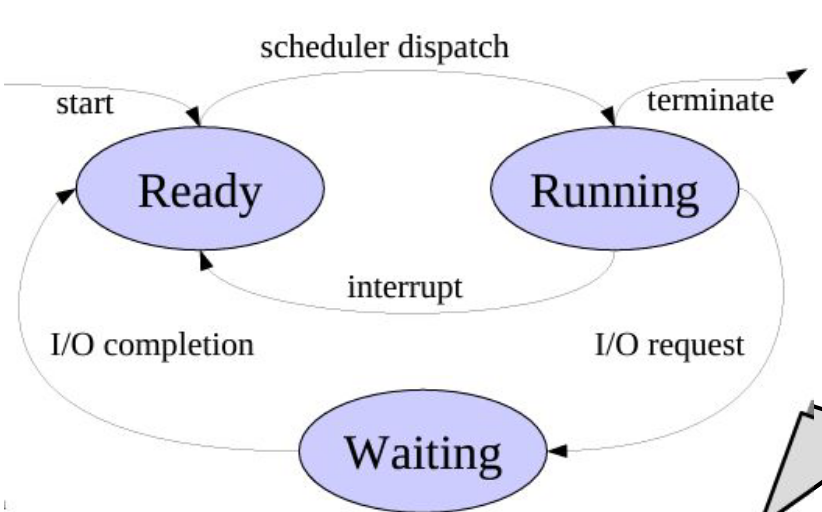
\includegraphics[width=0.5\linewidth]{Images/Screenshot 2024-12-26 at 15-07-23 so-03.1-concorrenza - so-03.1-concorrenza.pdf.png}
\end{figure}

\subsection{Multiprogramming e multiprocessing}

\subsubsection{Cos'è la concorrenza?}

Tema centrale nella progettazione dei S.O. riguarda la gestione
di processi multipli.

Due programmi si dicono in esecuzione concorrente se vengono
eseguiti in parallelo (con parallelismo reale o apparente).
La concorrenza è l'insieme di notazioni per descrivere l'esecuzione concorrente di due o più programmi, sono tecniche per risolvere i problemi associati all'esecuzione concorrente, quali comunicazione e sincronizzazione.
\newline

La multiprogrammazione è stata inventata affinchè più processi
indipendenti condividano il processore. Alcune
applicazioni possono essere progettate come un insieme di processi
o thread concorrenti.

Inoltre, molte funzioni del sistema operativo possono essere implementate come un insieme di processi o thread.

\begin{itemize}
    \item \textbf{Multiprogramming:} più processi su un solo processore, parallelismo apparente.
    \item \textbf{Multiprocessing:} più processi su una macchina con processori multipli, parallelismo reale.
    \item \textbf{Distributed processing:} più processi su un insieme di computer distribuiti e indipendenti, parallelismo reale.
\end{itemize}

\subsubsection{Differenze tra multiprocessing e multiprogramming}
\paragraph{In un singolo processore:}processi multipli sono "alternati nel tempo" per dare l'impressione di
avere un multiprocessore. Ad ogni istante, al massimo un processo è in esecuzione, si parla di \textbf{interleaving}.

\paragraph{In un sistema multiprocessore:}più processi vengono eseguiti simultaneamente su processori diversi, i processi sono "alternati nello spazio e si parla di \textbf{overlapping}.

\paragraph{}
A prima vista si potrebbe pensare che queste differenze comportino
problemi distinti.
In un caso l'esecuzione è simultanea, nell'altro caso la simultaneità è solo simulata.

In realtà presentano gli stessi problemi, ovvero, non è possibile predire la velocità relativa dei processi.

\paragraph{Alcune considerazioni:} non vi è sostanziale differenza tra i problemi relativi a multiprogramming e multiprocessing, ai fini del ragionamento sui programmi concorrenti si ipotizza che sia
presente un "processore ideale" per ogni processo.

I problemi derivano dal fatto che non è possibile predire gli istanti temporali in cui vengono eseguite le istruzioni i due processi quando accedono ad una o più risorse condivise.

\subsubsection{Race condition}
\paragraph{Definizione:}si dice che un sistema di processi multipli presenta una race condition qualora il risultato finale dell'esecuzione dipenda dalla temporizzazione con cui vengono eseguiti i processi.
\paragraph{}
Per scrivere un programma concorrente è necessario eliminare le race condition.
\newline
In pratica scrivere programmi concorrenti è più difficile che scrivere programmi sequenziali.
La correttezza non è solamente determinata dall'esattezza dei passi
svolti da ogni singola componente del programma, ma anche dalle
interazioni (volute o no) tra essi.
Fare debug di applicazioni che presentano race condition non
è per niente piacevole...

\subsubsection{Notazione per descrivere processi concorrenti}

\begin{lstlisting}
    process nome {
... statement(s) ...
}
\end{lstlisting}

Esempio

\begin{lstlisting}
process P1 {
    totale = totale + valore;
}

process P2 {
    totale = totale - valore;
}
\end{lstlisting}

\section{Interazioni tra processi}

E' possibile classificare le modalità di interazione tra processi
in base a quanto sono "consapevoli" l’uno dell'altro.


\subsection{Tipi di interazione}
\subsubsection{Processi ignari}
Processi totalmente "ignari" l’uno dell'altro non sono progettati per lavorare insieme, sebbene siano indipendenti, vivono in un ambiente comune.
\paragraph{Come interagiscono?} essi competono per le stesse risorse e devono sincronizzarsi nella loro utilizzazione. Il sistema operativo ha il compito di arbitrare questa competizione, fornendo meccanismi di sincronizzazione.

\subsubsection{Processi indiretti}
Mentre processi "indirettamente" a conoscenza uno dell'altro
sono processi che condividono risorse, come ad esempio un buffer, al fine di scambiarsi informazioni, non si conoscono in base ai loro id, ma interagiscono indirettamente tramite le risorse condivise.
\paragraph{Come interagiscono?} cooperano per qualche scopo e devono sincronizzarsi nella utilizzazione delle risorse. Il sistema operativo deve facilitare la cooperazione, fornendo meccanismi di sincronizzazione.

\subsubsection{Processi diretti}
Processi "direttamente" a conoscenza uno dell'altro sono coloro che comunicano uno con l'altro sulla base dei loro id, la comunicazione è diretta, spesso basata sullo scambio di messaggi
\paragraph{Come interagiscono?} cooperano per qualche scopo e comunicano informazioni agli altri processi.
Il sistema operativo deve facilitare la cooperazione, fornendo meccanismi di comunicazione.

\subsection{Proprietà fondamentali}
\paragraph{Definizione:}una proprietà di un programma concorrente è un attributo che rimane vero per ogni possibile storia di esecuzione del programma stesso.

Esistono due tipi di proprietà:
\begin{itemize}
    \item \textbf{Safety ("nothing bad happens"): }mostrano che il programma (se avanza) va "nella direzione voluta", cioè
non esegue azioni scorrette.
    \item \textbf{Liveness ("something good eventually happens"): }il programma avanza, non si ferma... insomma è “vitale.
\end{itemize}

Esempio: \textbf{Consensus }
\newline
Si consideri un sistema con N processi: all'inizio, ogni processo propone un valore. Alla fine, tutti i processi si devono accordare su uno dei valori proposti (decidono quel valore).
\newline

\textbf{Proprietà di safety: }se un processo decide, deve decidere uno dei valori proposti, se due processi decidono, devono decidere lo stesso valore.
\newline

\textbf{Proprietà di liveness: } prima o poi ogni processo corretto \textit{(i.e. non in crash)} prenderà una decisione.

\subsubsection{Proprietà - programmi sequenziali}
Nei programmi sequenziali le \textbf{proprietà di safety} esprimono la correttezza dello stato finale (il risultato è quello voluto).
La principale \textbf{proprietà di liveness} è la terminazione.

\subsubsection{Proprietà - programmi concorrenti}
\paragraph{Proprietà di safety:} i processi non devono "interferire" fra di loro nell'accesso alle risorse
condivise, questo vale ovviamente per i processi che condividono risorse (non per processi che cooperano tramite comunicazione).
I meccanismi di sincronizzazione servono a garantire la
proprietà di safety, devono essere usati propriamente dal programmatore, altrimenti il programma potrà contenere delle race conditition.

\paragraph{Proprietà di liveness:} i meccanismi di sincronizzazione utilizzati non devono prevenire l'avanzamento del programma. Non è possibile che tutti i processi si "blocchino", in attesa di eventi che non possono verificarsi perché generabili solo da altri processi bloccati.
Non è possibile che un processo debba "attendere indefinitamente"
prima di poter accedere ad una risorsa condivisa.

\subsection{Mutua esclusione}
\paragraph{Definizione:} l'accesso ad una risorsa si dice mutualmente esclusivo se ad ogni istante, al massimo un processo può accedere a quella risorsa.

\textit{Esempi da considerare: due processi che vogliono accedere contemporaneamente a una stampante. Due processi che cooperano scambiandosi informazioni tramite un buffer condiviso.}

\subsection{Deadlock (stallo)}
La mutua esclusione permette di risolvere il problema della non
interferenza, ma può causare il blocco permanente dei processi.
\newline

Esempio:
Siano $R_1$ e $R_2$ due risorse.
Siano $P_1$ e $P_2$ due processi che devono accedere a $R_1$ e $R_2$ contemporaneamente, prima di poter terminare il programma.

Supponiamo che il S.O. assegni $R_1$ a $P_1$, e $R_2$ a $P_2$
\newline

I due processi sono bloccati in attesa circolare, si dice che $P_1$ e $P_2$ sono in \textbf{deadlock}.
E' una condizione definitiva da evitare.
Nei sistemi reali, se ne può uscire solo con metodi "distruttivi", ovvero uccidendo i processi, riavviando la macchina, etc.

\subsection{Starvation (inedia)}
Il deadlock è un problema che coinvolge tutti i processi che utilizzano un certo insieme di risorse. Esiste anche la possibilità che un processo non possa accedere ad una risorsa perché "sempre occupata".

\textit{Esempio: se siete in coda ad uno sportello e continuano ad arrivare "furbi" che passano davanti, non riuscirete mai a parlare con l'impiegato.}
\newline

Esempio:
Sia R una risorsa.
Siano $P_1$, $P_2$ e $P_3$ tre processi che devono accedere periodicamente a R.
\newline

Supponiamo che $P_1$ e $P _2$ si alternino nell'uso della risorsa
$P_3$ non può accedere alla risorsa, perché utilizzata in modo esclusivo dagli altri due processi.

Si dice che $P_3$ è in \textbf{starvation}.
A differenza del deadlock, non è una condizione definitiva è possibile uscirne, basta adottare un'opportuna politica di assegnamento.
Rimane comunque una situazione da evitare.

\subsection{Azioni atomiche}
\paragraph{Definizione:} le azioni atomiche vengono compiute in modo indivisibile, soddisfano la condizione: o tutto o niente.
Nel caso di parallelismo reale si garantisce che l'azione non interferisca con altri processi durante la sua esecuzione.
Nel caso di parallelismo apparente l'avvicendamento (context switch) fra i processi avviene prima o dopo l'azione, che quindi non può interferire.
\newline

Esempi:
Le singole istruzioni del linguaggio macchina sono atomiche
\begin{lstlisting}
     sw $a0, ($t0)
\end{lstlisting}

\paragraph{Nel caso di parallelismo apparente:}il meccanismo degli interrupt (su cui è basato l'avvicendamento dei processi) garantisce che un interrupt venga eseguito prima o dopo un'istruzione, mai "durante".

\paragraph{Nel caso di parallelismo reale:} anche se più istruzioni cercano di accedere alla stessa cella di
memoria (quella puntata da $t0$), la politica di arbitraggio del bus garantisce che una delle due venga servita per prima e l'altra
successivamente.
\newline

Controesempi:
In generale, sequenze di istruzioni in linguaggio macchina non
sono azioni atomiche
\begin{lstlisting}
    lw $t0, ($a0)
    add $t0, $t0, $a1
    sw $t0, ($a0)
\end{lstlisting}
\textit{(Attenzione però: le singole istruzioni in linguaggio macchina sono atomiche, le singole istruzioni in assembly possono non essere atomiche!)}
\newline

E nei compiti di concorrenza?
Assumiamo che in ogni istante, vi possa essere al massimo un accesso alla memoria alla volta.

Questo significa che operazioni tipo: aggiornamento di una variabile, incremento di una variabile e valutazione di espressioni
\textbf{non sono atomiche}.

Operazioni tipo: assegnamento di un valore costante ad una variabile, \textbf{sono atomiche}.

\subsubsection{Annotazione}
Nel seguito, utilizzeremo la notazione \textbf{$<S>$} per indicare che lo statement S deve essere eseguito in modo atomico
\newline

Esempio:
\begin{lstlisting}
    < x = x + 1; >
\end{lstlisting}

\section{Sezioni critiche}

\subsubsection{Non interferenza}
Se le sequenze di istruzioni non vengono eseguite in modo atomico,
come possiamo garantire la non-interferenza?

Dobbiamo trovare il modo di specificare che certe parti dei programmi sono "speciali", ovvero devono essere eseguite in modo atomico (senza interruzioni).

\paragraph{Definizione:} La parte di un programma che utilizza una o più risorse condivise viene detta \textbf{sezione critica} (critical section, o \textbf{CS}).
\newline

Esempio:
\begin{lstlisting}
    process P1 {
        a1 = rand();
        totale = totale + a1; //CS
    }

    process P2 {
        a2 = rand();
        totale = totale + a2; //CS
}
\end{lstlisting}

La parte evidenziata è una sezione critica, in quanto accede alla
risorsa condivisa totale; mentre a1 e a2 non sono condivise.

\paragraph{Obiettivi:}Vogliamo garantire che le sezioni critiche siano eseguite in modo
mutualmente esclusivo (atomico) evitando così situazioni di blocco, sia dovute a deadlock sia dovute a starvation.

\paragraph{Sintassi:}
\begin{itemize}
    \item \textbf{[enter cs]} indica il punto di inizio di una sezione critica.
    \item \textbf{[exit cs]} indica il punto di fine di una sezione critica.
\end{itemize}

Perché abbiamo bisogno di costrutti specifici? Perché il S.O. non può capire da solo cosa è una sezione critica e cosa non lo è.

Esempio:
\begin{lstlisting}
    x=0
    cobegin
        [enter cs]; x = x+1; [exit cs];

        [enter cs]; x = x+1; [exit cs];
    coend
\end{lstlisting}

\subsubsection{Requisiti delle CS}
Si tratta di realizzare N processi della forma:
\begin{lstlisting}
    process Pi { // i=1...N 
        while (true) {
        [enter cs]
            critical section
        [exit cs]
            non-critical section
        }
    }       
\end{lstlisting}
  
In modo che valgano le seguenti proprietà:
\begin{enumerate}
    \item \textbf{Mutua esclusione:} solo un processo alla volta deve essere all'interno della CS, fra tutti quelli che hanno una CS per la stessa risorsa condivisa.
    \item \textbf{Assenza di deadlock:} uno scenario in cui tutti i processi restano bloccati definitivamente non è ammissibile.
    \item \textbf{Assenza di delay non necessari:} un processo fuori dalla CS non deve ritardare l'ingresso della CS da parte di un altro processo.
    \item \textbf{Eventual entry (assenza di starvation:)} ogni processo che lo richiede, prima o poi entra nella CS.
\end{enumerate}
 \textit{N.B: Se un processo entra in una critical section, prima o poi ne uscirà, quindi esso può terminare solo fuori dalla sua sezione critica!}

 \subsubsection{Possibili approcci}
 \begin{itemize}
    \item \textbf{Approcci software:} la responsabilità cade sui processi che vogliono accedere ad un oggetto distribuito, Può essere soggetto ad errori e vedremo che è costoso in termini di esecuzione (busy waiting).
    \item \textbf{Approcci hardware:} utilizza istruzioni speciali del linguaggio macchina, progettate apposta. Sono efficienti ma non sono adatti come soluzioni general-purpose.
    \item \textbf{Approcci basati su supporto nel S.O. o nel linguaggio:} la responsabilità di garantire la mutua esclusione ricade sul S.O. o sul linguaggio.
    \textit{Esempi: semafori, monitor message passing.}
 \end{itemize}
\newpage

\subsection{Tecniche software: Algoritmo di Dekker}
\begin{lstlisting}
    shared int turn = P;
    shared boolean needp = false; shared boolean needq = false;
    
    cobegin P -> Q coend
        
        process P {
            while (true) {
                // entry protocol 
                needp = true;
                while (needq)
                    if (turn == Q) {
                        needp = false;
                        while (turn == Q);
                            // do nothing 
                        needp = true;
                    }
                //critical section
                needp = false; turn = Q;
                //non-critical section
            }
        }

        process Q {
            while (true) {
                // entry protocol 
                needq = true;
                while (needp)
                    if (turn == P) {
                        needq = false;
                        while (turn == P); 
                            // do nothing
                        needq = true;
                    }
                //critical section
                needq = false; turn = P;
                //non-critical section
            }
        }
\end{lstlisting}

\subsubsection{Dimostrazione (mutua esclusione)}

Per assurdo supponiamo che P e Q siano in CS contemporaneamente.
Poiché gli accessi in memoria sono esclusivi, per entrare devono almeno aggiornare / valutare entrambe le variabili needp e needq.

Uno dei due entra per primo; diciamo sia Q: needq sarà true fino a quando Q non uscirà dal ciclo, poiché P entra nella CS mentre Q è nella CS, significa che esiste un istante temporale in cui needq = false e Q è in CS.
\newline
ASSURDO!

\subsubsection{Dimostrazione (assenza di deadlock)}
Per assurdo supponiamo che né P né Q possano entrare in CS. P e Q devono essere bloccati nel primo while, esiste un istante t dopo di che needp e needq sono sempre true.

Supponiamo che all'istante t, turn = Q.
L'unica modifica a turn può avvenire solo quando Q entra in CS, dopo t, turn resterà sempre uguale a Q, P entra nel primo ciclo, e mette needp = false.
\newline
ASSURDO!

\subsubsection{Dimostrazione (assenza di ritardi non necessari)}
Se Q sta eseguendo codice non critico, allora needq = false.
Allora P può entrare nella CS.

\subsubsection{Dimostrazione (assenza di starvation)}
Se Q richiede di accedere alla CS: needq = true.
Se P sta eseguendo codice non critico: Q entra
Se P sta eseguendo il resto del codice (CS, entrata, uscita): prima o poi ne uscirà e metterà il turno a Q.
Q potrà quindi entrare.

\subsection{Tecniche software: Algoritmo di Peterson}
Più semplice e lineare di quello di Dijkstra / Dekker
e facilmente generalizzabile al caso di processi multipli.

\begin{lstlisting}
    shared boolean needp = false;
    shared boolean needq = false;
    shared int turn;
    
    cobegin P -> Q coend
        
        process P {
            while (true) {
                // entry protocol
                needp = true;
                turn = Q;
                while (needq && turn != P); 
                    // do nothing
                //critical section
                needp = false;
                //non-critical section
            }
        }

        process Q {
            while (true) {
                // entry protocol
                needq = true;
                turn = P;
                while (needp && turn != Q);
                    //do nothing
                //critical section
                needq = false;
                //non-critical section
            }
        }
\end{lstlisting}

\subsubsection{Dimostrazione (mutua esclusione)}
Supponiamo che P sia entrato nella sezione critica.

Vogliamo provare che Q non può entrare, sappiamo che needP == true
e Q entra solo se turn = Q quando esegue il while.
Si consideri lo stato al momento in cui P entra nella critical section.

Ho due possibilità, needq == false or turn == P:
\begin{itemize}
    \item Se needq == false, Q doveva ancora eseguire needq == true, e quindi lo eseguirà dopo l'ingresso di P e porrà turn=P, precludendosi la possibilità di entrare.
    \item Se turn==P, come sopra;
\end{itemize}




\subsubsection{Dimostrazione (assenza di deadlock)}

Supponiamo che per assurdo che P voglia entrare nella CS e sia
bloccato nel suo ciclo while, questo significa che: needp = true, needq = true, turn = Q per sempre.

Possono darsi tre casi:
\begin{itemize}
    \item Q non vuole entrare in CS: impossibile, visto che needq = true
    \item Q è bloccato nel suo ciclo while: impossibile, visto che turn = Q
    \item Q è nella sua CS e ne esce (prima o poi): impossibile, visto che prima o poi needq assumerebbe il valore false
\end{itemize}

\subsubsection{Dimostrazione (assenza di ritardi non necessari)}
Se Q sta eseguendo codice non critico, allora needq = false, allora P può entrare nella CS.

\subsubsection{Dimostrazione (assenza di starvation)}
Simile alla dimostrazione di assenza di deadlock, aggiungiamo un caso in fondo:
Q continua ad entrare ed uscire dalla sua CS, prevenendo l'ingresso di P.

Impossibile poiché quando Q prova ad entrare nella CS pone turn = P
siccome needp = true e  quindi Q deve attendere che P entri nella CS.

\subsection{Algoritmo di Peterson – Generalizzazione per N processi}

\begin{lstlisting}
    shared int[] stage = new int[N]; /* 0-initialized */
    shared int[] last = new int[N]; /* 0-initialized */
    
    cobegin P0 -> P1 -> ... -> PN-1 coend

    process Pi { // i = 0...N-1 
        while (true) {
        // Entry protocol
        for (int j=0; j < N; j++) {
            stage[i] = j; last[j] = i;
            for (int k=0; k < N; k++) {
                if (i != k){
                    while (stage[k] >= stage[i] && last[j] == i)
                    ;
                    }
                }
        }
        //critical section
        stage[i] = 0;
        //non-critical section
        }
    }
\end{lstlisting}



\subsection{Tecniche hardware: disabilitazione interrupt, istruzioni speciali}
Le soluzioni di Dekker e Peterson prevedono come uniche istruzioni
atomiche le operazioni di Load e Store. Si può pensare di fornire alcune istruzioni hardware speciali per semplificare la realizzazione di sezioni critiche.
Nei sistemi uniprocessore, i processi concorrenti vengono "alternati" tramite il meccanismo degli interrupt.
Possiamo quindi disabilitarli.
\newline

\textit{Esempio:}

\begin{lstlisting}
    process P {
        while (true) {
            //disable interrupt
            critical section

            //enable interrupt
            non-critical section
        }
    }
\end{lstlisting}ù

Il problema è che il S.O. deve lasciare ai processi la responsabilità di riattivare gli interrupt ciò è altamente pericoloso perchè riduce il grado di parallelismo ottenibile dal processore. Inoltre non funziona su sistemi multiprocessore.
\newpage

\subsubsection{Test e Set}
Test e Set sono istruzioni che realizzano due azioni in modo atomico.
\textit{Esempi: lettura e scrittura, test e scrittura.}

$TS(x,y) := < y = x ; x = 1 >$
\newline
Esso ritorna in y il valore precedente di x e assegna 1 ad x.

\begin{lstlisting}
    shared lock=0; cobegin P -> Q coend
    
    process P {
        int vp;
        while (true) {
            do {
                TS(lock, vp);
            } while (vp);
            
            //critical section
            lock=0;
            //non-critical section
        }
    }

    process Q {
        int vp;
        while (true) {
            do {
                TS(lock, vp);
            } while (vp);
            
            //critical section
            lock=0;
            //non-critical section
        }
    }
\end{lstlisting}

\paragraph{Rispetta tutti i requisiti delle CS:}
\begin{itemize}
    \item Mutua esclusione: entra solo chi riesce a settare per primo il lock.
    \item No deadlock: il primo che esegue TS entra senza problemi.
    \item No unnecessary delay: un processo fuori dalla CS non blocca gli altri.
    \item No starvation: no, se non assumiamo qualcosa di più.
\end{itemize}

\subsubsection{Riassumendo}
\begin{itemize}
    \item \textbf{Vantaggi delle istruzioni speciali hardware:}
    \begin{itemize}
        \item sono applicabili a qualsiasi numero di processi, sia su sistemi monoprocessore che in sistemi multiprocessori.
        \item semplice e facile da verificare.
        \item può essere utilizzato per supportare sezioni critiche multiple; ogni sezione critica può essere definita dalla propria variabile.
    \end{itemize}
    \item \textbf{Svantaggi:}
    \begin{itemize}
        \item si utilizza ancora busy-waiting.
        \item i problemi di starvation non sono eliminati.
        \item sono comunque complesse da programmare.
    \end{itemize}
\end{itemize}

\section{Semafori}
Due o più processi possono cooperare attraverso semplici segnali, in modo tale che un processo possa essere bloccato in specifici punti del suo programma finché non riceve un segnale da un altro processo.

\subsection{Definizione}
E' un tipo di dato astratto per il quale sono definite due operazioni:
\begin{itemize}
    \item  \textbf{V} (dall'olandese verhogen): viene invocata per inviare un segnale, quale il verificarsi di un evento o il rilascio di una risorsa.
    \item  \textbf{P} (dall'olandese proberen): viene invocata per attendere il segnale (ovvero, per attendere un evento o il rilascio di una risorsa).
\end{itemize}

Un semaforo può essere visto come una variabile intera, che viene inizializzata ad un valore non negativo.
L'operazione P attende che il valore del semaforo sia positivo e decrementa il valore del semaforo.
L'operazione V incrementa il valore del semaforo.

\textit{N.B: le azioni P e V sono atomiche}

\begin{lstlisting}
    class Semaphore {
    private int val;
    Semaphore(int init) { }
        void P() {}
        void V() {}
}
\end{lstlisting}

\subsubsection{Semaforo - Invariante}

Siano:
\begin{itemize}
    \item $n_P$ il numero di operazioni P completate
    \item $n_V$ il numero di operazioni V completate
    \item init il valore iniziale del semaforo
\end{itemize}

Vale il seguente invariante: $n_P \leq n_V + init$

Due casi:
\begin{itemize}
    \item \textbf{eventi ($init = 0$)} : il numero di eventi "consegnati" deve essere non superiore al numero di volte che l'evento si è verificato.
    \item \textbf{risorse ($init \geq 0$)} : il numero di richieste soddisfatte non deve essere superiore al numero iniziale di risorse + il numero di risorse restituite.
\end{itemize}

\subsubsection{Implemetazione di CS}
\begin{lstlisting}
    Semaphore s = new Semaphore(1);

        process P {
            while (true) {
                s.P();
                //critical section
                s.V();
                //non-critical section
            }
        }
\end{lstlisting}

\subsubsection{Politiche di gestione dei processi bloccati}
Per ogni semaforo, il S.O. deve mantenere una struttura dati contenente l'insieme dei processi sospesi. Quando un processo deve essere svegliato, è necessario selezionare uno dei processi sospesi.

I \textbf{semafori FIFO} adottano la politica first-in, first-out.
Il processo che è stato sospeso più a lungo viene svegliato per primo, è una politica fair, che garantisce assenza di starvation, la struttura dati è una coda.
Se non viene specificata l'ordine in cui vengono rimossi, i semafori possono dare origine a starvation.
\newline

Da ora in poi utilizzeremo solo i semafori FIFO...
\newpage

\subsection{Implementazione}

\subsubsection{La funzione P}

\begin{lstlisting}
    void P() {
        value--;
        if (value < 0) {
            pid = <id del processo che ha invocato P>;
            queue.add(pid);
            suspend(pid);
        }
    }
\end{lstlisting}    

\textbf{Riga 5} Il process id del processo bloccato viene messo in un insieme queue.

\textbf{Riga 6} Con l'operazione suspend, il s.o mette il processo nello stato waiting.

\subsubsection{La funzione V}

\begin{lstlisting}
    void V() {
        value++;
        if (value <= 0){
            pid = queue.remove();
            wakeup(pid);
        }
    }
\end{lstlisting}

\textbf{Riga 4} Il process id del processo da sbloccare viene selezionato dall'insieme queue.

\textbf{Riga 5} Con l'operazione wakeup, il S.O. mette il processo nello stato ready.
\newline

Quindi è necessario utilizzare una delle tecniche di critical section viste in precedenza: Dekker, Peterson oppure test-set, swap, etc.

\begin{lstlisting}
    void P() {
        //[enter CS]
        value--;
        if (value < 0) {
            int pid = <id del processo che ha invocato P>;
            queue.add(pid);
            suspend(pid);
        }
        //[exit CS]
    }
    

    void V() {
        //[enter CS]
        value++;
        if (value <= 0){
            int pid = queue.remove();
            wakeup(pid);
        }
        //[exit CS]
    }
\end{lstlisting}

Utilizzando queste tecniche, abbiamo limitato busy-waiting alle sezioni critiche di P e V, e queste sezioni critiche sono molto brevi, in questo modo la sezione critica non è quasi mai occupata
e busy waiting avviene raramente.

\subsection{Semafori binari}

\paragraph{Definizione:}variante dei semafori in cui il valore può assumere solo i valori 0 e 1.

\paragraph{A cosa servono?}servono a garantire mutua esclusione, semplificando il lavoro del programmatore.
Hanno lo stesso potere espressivo dei semafori "normali".

\paragraph{Invariante dei semafori binari:}
$0 \leq n_V + init - n_P \leq 1$ oppure $0 \leq s.value \leq 1$
\newpage

\subsubsection{Implementazione nei sistemi operativi}
\begin{lstlisting}
    class BinarySemaphore {
        private int value;
        Queue queue0 = new Queue();
        Queue queue1 = new Queue();
        BinarySemaphore() { value = 1; }

        void P() {
            //[enter CS]
            int pid = <process id>;
            if (value == 0) {
                queue0.add(pid);
                suspend(pid);
            }
            value--;
        
            if (queue1.size() > 0) {
                int pid = queue1.remove();
                wakeup(pid);
            }
            //[exit CS]
        }

        void V() {
            //[enter CS]
            int pid = <process id>;
            if (value == 1) {
                queue1.add(pid);
                suspend(pid);
            }
            value++;
            
            if (queue0.size() > 0) {
                int pid = queue0.remove();
                wakeup(pid);
            }
            //[exit CS]
        }
\end{lstlisting}

\subsubsection{Implementazione tramite semafori generali}
\begin{lstlisting}
    class BinarySemaphore {
        private Semaphore s0 , s1 ;
        int value ;

        BinarySemaphore(int v){ //fail if v not in {0,1}
            s0 = new Semaphore(v)
            s0 = new Semaphore(1-v)
        }
        
        void P(void){
            s0.P();
            s1.V();
        }

        void V(void){
            s1.P();
            s0.V();
        }
    }
\end{lstlisting}

\section{Problemi classici}
Esistono un certo numero di problemi "classici" della programmazione concorrente:
\begin{itemize}
    \item producer/consumer
    \item bounded buffer
    \item dining philosophers
    \item readers/writers
\end{itemize}

Nella loro semplicità rappresentano le interazioni tipiche dei processi concorrenti.

\subsection{Producer/Consumer}

\paragraph{Definizione:} esiste un processo "produttore" \textbf{Producer} che genera valori (record, caratteri, oggetti, etc.) e vuole trasferirli a un processo "consumatore" \textbf{Consumer} che prende i valori generati e li "consuma".
La comunicazione avviene attraverso una singola variabile condivisa.

\paragraph{Proprietà da garantire:} Producer non deve scrivere nuovamente l'area di memoria condivisa prima che Consumer abbia effettivamente utilizzato il valore precedente.
Consumer non deve leggere due volte lo stesso valore, ma deve attendere che Producer abbia generato il successivo.
Assenza di deadlock.

\begin{lstlisting}
    shared Object buffer;
    Semaphore empty = new Semaphore(1);
    Semaphore full = new Semaphore(0);

    //cobegin
        Producer
        ....
        Consumer
    //coend

    process Producer {
        while (true) {
            Object val = produce();
            empty.P();
            buffer = val;
            full.V();
        }
    }
    
    process Consumer {
        while (true) {
            full.P();
            Object val = buffer;
            empty.V();
            consume(val);
        }
    }

\end{lstlisting}


\subsection{Bounded Buffer}
\paragraph{Definizione:} è simile al problema del produttore/consumatore.
In questo caso, però, lo scambio tra produttore e consumatore non
avviene tramite un singolo elemento, ma tramite un buffer di
dimensione limitata, i.e. un vettore di elementi.
\paragraph{Proprietà da garantire:} Producer non deve sovrascrivere elementi del buffer prima che Consumer abbia effettivamente utilizzato i relativi valori.
Consumer non deve leggere due volte lo stesso valore, ma deve
attendere che Producer abbia generato il successivo.
Assenza di deadlock e assenza di starvation.

\subsubsection{Struttura del buffer}
Array circolare: si utilizzano due indici front e rear che indicano rispettivamente il prossimo elemento da scrivere e il prossimo elemento da leggere. Gli indici vengono utilizzati in modo ciclico (modulo l'ampiezza del buffer).

\textit{Esempi:}
\begin{figure} [h]
    \centering
    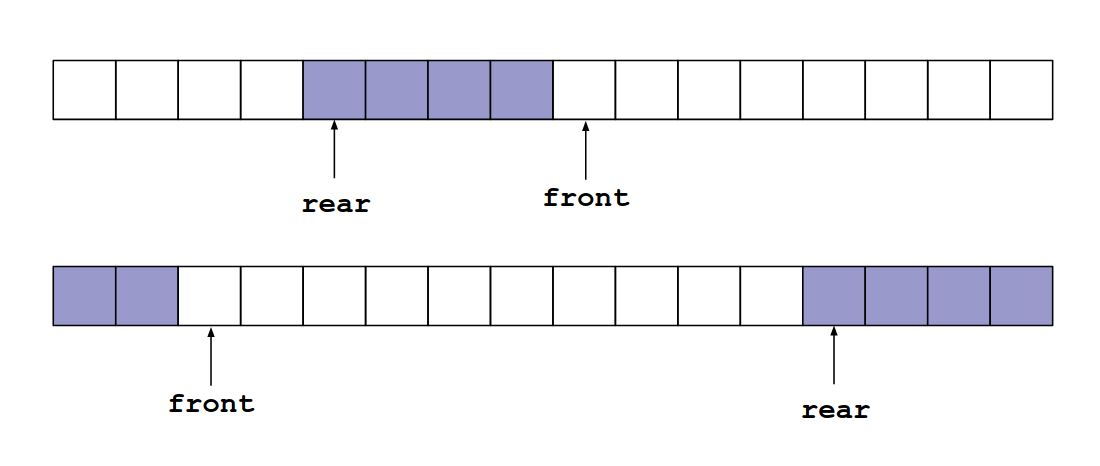
\includegraphics[width=0.5\linewidth]{Images/Screenshot 2024-12-28 at 19-31-02 so-03.1-concorrenza - so-03.1-concorrenza.pdf.png}
\end{figure}

\begin{lstlisting}
    Object buffer[SIZE];
    int front = 0;
    int rear = 0;
    Semaphore empty = new Semaphore(SIZE);
    Semaphore full = new Semaphore(0);

    process Producer {
        while (true) {
            Object val = produce();
            empty.P();
            buf[front] = val;
            front = (front + 1) % SIZE;
            full.V();
        }
    }

    process Consumer {
        while (true) {
            full.P();
            Object val = buf[rear];
            rear = (rear + 1) % SIZE;
            empty.V();
            consume(val);
        }
    }
\end{lstlisting}

\subsection{Cena dei Filosofi}
\paragraph{Descrizione:}Cinque filosofi passano la loro vita a pensare e a mangiare (alternativamente).
Per mangiare fanno uso di una tavola rotonda con 5 sedie, 5 piatti e 5 posate fra i piatti.
Per mangiare, un filosofo ha bisogno di entrambe le posate (destra/sinistra), per pensare, un filosofo lascia le posate
dove le ha prese.

I problemi produttore/consumatore e buffer limitato mostrano come risolvere il problema di accesso esclusivo a una o più
risorse indipendenti.

Il problema dei filosofi mostra come gestire situazioni in cui i processi entrano in competizione per accedere ad insiemi di risorse a intersezione non nulla.

\subsubsection{La vita di un filosofo}
\begin{lstlisting}
    process Philo[i] { /* i = 0...4 */
        while (true) {
            //think
            //acquire chopsticks
            //eat
            //release chopsticks
        }
    }
\end{lstlisting}        

Le bacchette vengono denominate: \textbf{chopstick[i]} con i=0...4;
Il filosofo i accede alle posate chopstick[i] e chopstick[(i+1) \% 5];
\subsubsection{Invarianti}
$up_i$ il numero di volte che la bacchetta i viene preso dal tavolo
$down_i$ il numero di volte che la bacchetta i viene rilasciata sul tavolo
\newpage
\textbf{Invariante}
$down_i \leq up_i \leq down_i + 1$

Per comodità si può definire chopstick[i] = 1 - ($up_i-down_i$)
(può essere pensato come un semaforo binario)

\subsubsection{Soluzione}
\begin{lstlisting}
Semaphore chopsticks = { new Semaphore(1), ..., new Semaphore(1)};

    process Philo[0] {
        while (true) {
            //think
            chopstick[1].P();
            chopstick[0].P();
            //eat
            chopstick[1].V();
            chopstick[0].V();
        }
    }

    process Philo[i] { /* i = 1...4 */
        while (true) {
            //think
            chopstick[i].P();
            chopstick[(i+1)%5].P();
            //eat
            chopstick[i].V();
            chopstick[(i+1)%5].V();
        }
    }
\end{lstlisting}

\subsection{Lettori e scrittori}

\paragraph{Descrizione:} Un database è condiviso tra un certo numero di processi, esistono due tipi di processi.
I lettori accedono al database per leggerne il contenuto
e gli scrittori accedono al database per aggiornarne il contenuto.

\paragraph{Proprietà:} Se uno scrittore accede a un database per aggiornarlo, esso opera in mutua esclusione; nessun altro lettore o scrittore può accedere al database.
Se nessuno scrittore sta accedendo al database, un numero arbitrario di lettori può accedere al database in lettura.

\paragraph{Motivazioni:} La competizione per le risorse avviene a livello di classi di processi e non solo a livello di processi. Mostra che mutua esclusione e condivisione possono anche coesistere.

\paragraph{Invariante:} Sia \textbf{nr} il numero dei lettori che stanno accendo al database e sia \textbf{nw} il numero di scrittori che stanno accedendo al database.

L'invariante è il seguente: ($nr > 0$ \&\& $nw == 0$) $||$ ($nr == 0$ \&\& $nw \le 1$)

NOTA: il controllo può passare dai lettori agli scrittori o viceversa quando: $nr == 0$ \&\& $nw == 0$

\begin{lstlisting}
process Reader {
    while (true) {
        startRead();
        //read the database
        endRead();
    }
}

process Writer {
    while (true) {
        startWrite();
        //write the database
        endWrite();
    }
}
\end{lstlisting}

Note: startRead() e endRead() contengono le operazioni
necessarie affinché un lettore ottenga accesso al database.

startWrite() e endWrite() contengono le operazioni necessarie affinchè uno scrittore ottenga accesso al database.

\paragraph{}
Il problema dei lettori e scrittori ha molte varianti che si basano sui diversi concetti di priorità.

\subparagraph{Priorità ai lettori} Se un lettore vuole accedere al database, lo potrà fare senza attesa a
meno che uno scrittore non abbia già acquisito l'accesso al database. 

Scrittori hanno possibilità di starvation.
\subparagraph{Priorità agli scrittori} Uno scrittore attenderà il minimo tempo possibile prima di accedere al db.

Lettori hanno possibilità di starvation.

\subsubsection{Lettori e scrittori - Soluzione}

\begin{lstlisting}
/* Variabili condivise */
    int nr = 0;
    Semaphore rw = new
    Semaphore(1);
    Semaphore mutex = new
    Semaphore(1);

    void startRead() {
        mutex.P();
        if (nr == 0){
            rw.P();
            nr++;
            mutex.V();
        }
        void startWrite() {
        rw.P();
    }

    void endRead() {
        mutex.P();
        nr--;
        if (nr == 0) {
            rw.V();
            mutex.V();
        }

    void endWrite() {
        rw.V();
    }
\end{lstlisting}

Problemi: limitata a priorità per i lettori, di comprensione non semplice, non è chiaro da dove saltano fuori alcuni punti della soluzione.

\subsection{Come derivare una soluzione basata su semafori}
\subsubsection{Alcune definizioni utili - Andrews}
Sia \textbf{B} una \textbf{condizione booleana}.

Sia \textbf{S} uno \textbf{statement} (possibilmente composto)

Allora:
$< S >$ : esegui lo statement S in modo atomico.

$< await(B) \rightarrow S>$: attendi fino a che la condizione B è verificata e quindi esegui S. L'attesa e il comando vengono eseguiti in modo atomico, quindi, quando S viene eseguito, B è verificata.

\paragraph{Passi da seguire:}
\begin{enumerate}
    \item Definire il problema con precisione: identificare i processi, specificare i problemi di sincronizzazione, introdurre le variabili necessarie e definire un'invariante.
    \item Abbozzare una soluzione: produrre un primo schema di soluzione, e identificare le regioni che richiedono accesso atomico o mutualmente esclusivo.
    \item Garantire l'invariante: verifica che l'invariante sia sempre verificato
    \item Implementare le azioni atomiche: esprimere le azioni atomiche e gli statement \textbf{await} utilizzando le primitive di sincronizzazione disponibili.
\end{enumerate}

\subsubsection{Soluzione Lettori/Scrittori con Andrews}

\textbf{Variabili:} nr, nw - numero corrente di lettori/scrittori.
\newline
\textbf{Invariante:} ($nr > 0$ \&\& $nw == 0$) $||$ ($nr == 0$ \&\& $nw \le 1$)
\newline
\textbf{Schema della soluzione:}
\begin{lstlisting}
process Reader {
    < await (nw == 0) = nr++ >
    //read the database
    <nr-->
}

process Writer {
    < await (nr == 0 && nw == 0) = nw++ >
    //write the database
    <nw-->
}
\end{lstlisting}

dalla slide 142 alla 155 guardare sulle slide






\section{Conditional Critical Regions (CCR)}
\subsection{Introduzione}
I linguaggi di programmazione concorrente sono dotati di costrutti ad alto livello, che si propongono di prevenire la
possibilità di errori dovuti all'uso scorretto delle primitive.

I costrutti di programmazione concorrente sottraggono al programmatore la responsabilità dell'uso delle primitive
limitando così la possibilità di accessi indiscriminati ai dati comuni e favorendo la programmazione strutturata.

Questo è il compito del compilatore del linguaggio concorrente, che traduce i costrutti per la concorrenza in un insieme di primitive per la concorrenza.

Le \textbf{regioni critiche condizionali} sono costrutti che specificano operazioni su dati condivisi, da eseguire
in mutua esclusione, che possono determinare la sospensione e la riattivazione dei processi.

Forniscono una notazione più strutturata di quella dei semafori per specificare la sincronizzazione.

\subsubsection{Sintassi CCR} 

\lstinline{name (var declarations)}

\textbf{name} è un'identificatore per la risorsa condivisa.

\textbf{var declarations} è un'insieme di variabili condivise.
Dichiara che le variabili racchiuse tra parentesi sono condivise e devono essere accedute in mutua esclusione.

\lstinline{region name when condition do statement}
\textbf{condition} è una condizione booleana.
\lstinline{region name do statement}
\textbf{statement} è uno statement (potenzialmente composto) da eseguire. E' l'istruzione per acquisire la mutua esclusione su name.



\paragraph{L'esecuzione consiste in:}
\begin{itemize}
    \item Acquisire la mutua esclusione
    \item Valutare la condizione:
        \begin{itemize}
            \item se è falsa, rilasciare la mutua esclusione e ritardare fino a quando la condizione non è vera.
            \item se è vera, eseguire statement.
        \end{itemize}
\end{itemize}

\subsubsection{Vantaggi CCR}
Il compilatore del linguaggio attraverso il controllo dello scope delle variabili, può rilevare eventuali riferimenti illegittimi ai dati comuni.

\textit{Esempio: riferimenti non inclusi in regioni critiche condizionali associate al nome corretto}

Inoltre: "Compila" i costrutti region tramite le opportune chiamate a primitive di sincronizzazione (ad. es., semafori)

\subsubsection{Implementazione CCR tramite semafori}
Il ritardo di un processo che, all'interno della CCR, trovi la condizione falsa è realizzata con la sospensione fuori dalla mutua esclusione.

Una tecnica per rilevare la transizione al valore vero della condizione consiste nel far ripetere la verifica della condizione al processo medesimo, che naturalmente deve ri-accedere alla mutua esclusione.

\begin{lstlisting}
    resource name (var declarations)

/* Mutual exclusion semaphore, one for each critical region */
Semaphore mutex_name = new Semaphore(1);
/* Processes for which the condition is false must be
suspended */

Semaphore suspended_name = new Semaphore(0);
/* Number of suspended processes */
int nsuspended_name = 0;
/* Additional declarations */
var declarations
\end{lstlisting}

\begin{lstlisting}
    region name when condition do statement

    mutex_name.P();
    while (!condition) {
        /* condition is false */
        nsuspended_name++;
        mutex_name.V();
        suspended_name.P();
/* when process is reactived, it must re-gain access to the mutual exclusion */
        mutex_name.P();
    }

/* condition is true */
    statement;
/* after statement, one or more conditions may be true */
    while (nsuspended_name-- > 0)
        suspended_name.V();
\end{lstlisting}
\subsubsection{Schema CCR-Semafori}
\begin{figure} [h]
    \centering
    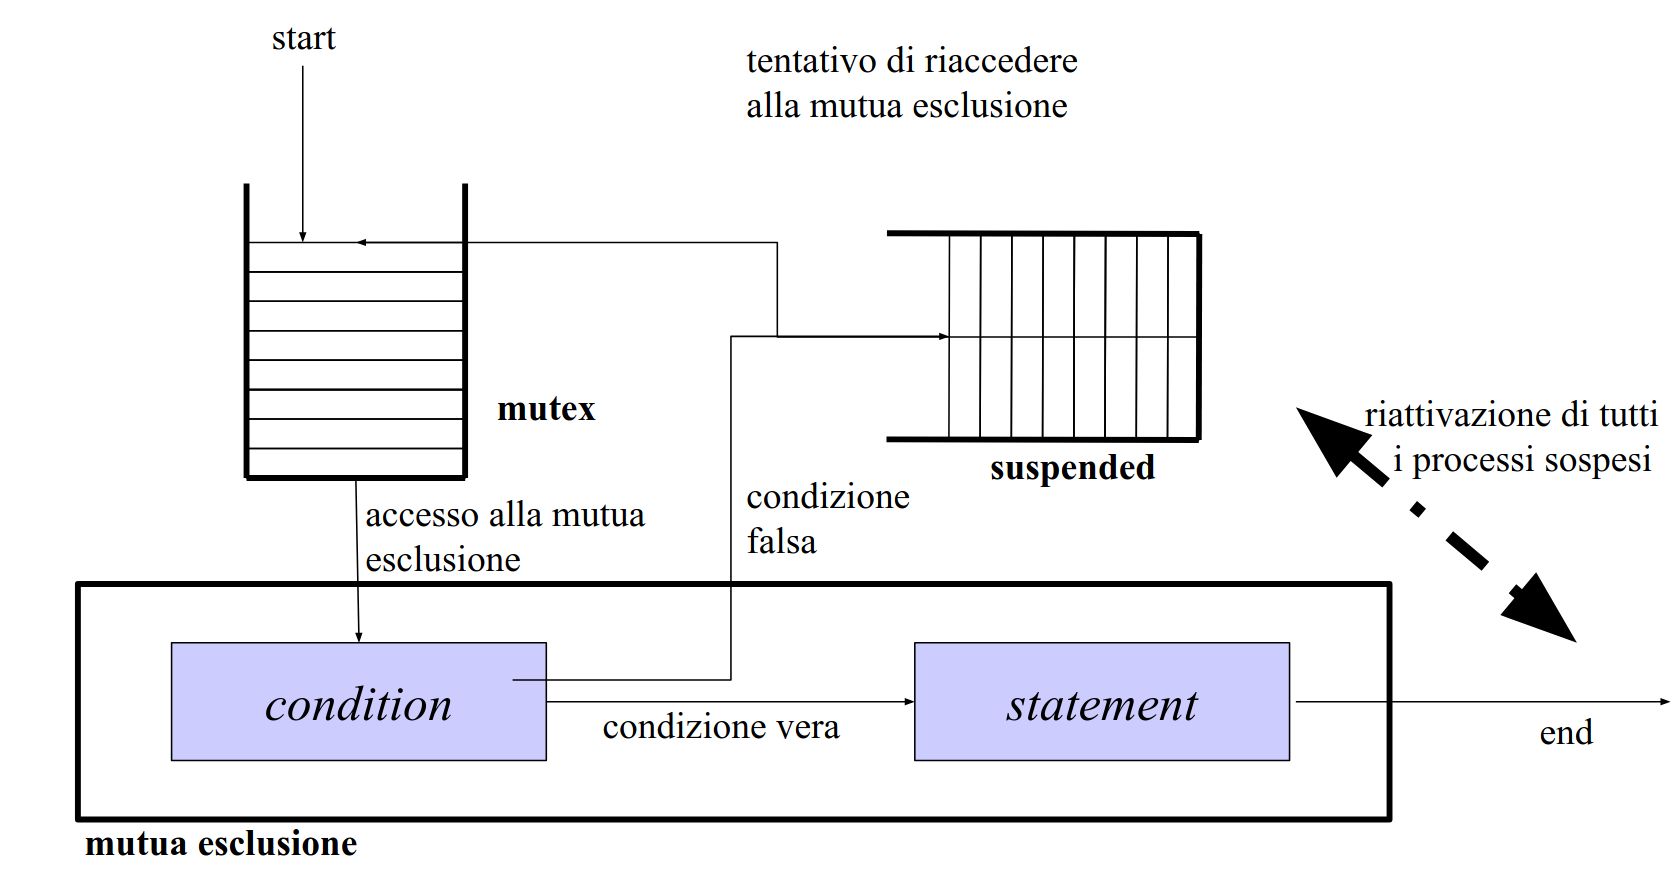
\includegraphics[width=0.85\linewidth]{Images/Screenshot 2025-01-16 at 12-03-09 so-03.1-concorrenza - so-03.1-concorrenza.pdf.png}
\end{figure}

\paragraph{Svantaggi:} questa realizzazione può risultare molto inefficiente nei sistemi uniprocessore, infatti, i processi possono essere riattivati ripetutamente prima di trovare la condizione vera.
Numerosi context switch del tutto improduttivi.

\paragraph{Vantaggi:} è più facile da realizzare qualora le condizioni siano complesse e coinvolgano variabili locali \textit{(non condivise)} dei processi coinvolti.

\subsection{CCR tramite semafori (passing the baton)}
\begin{lstlisting}
resource name (var declarations)

    Semaphore mutex_name = new Semaphore(1);
    Semaphore suspended_name[M_name] = { new Semaphore(0), ..., new Semaphore(0) };

    int nsuspended_name[M_name] = { 0, ..., 0 };
    //var declarations
\end{lstlisting}
dove $M_{name}$ è il numero di regioni critiche con condizione associate a \textbf{name.}

\begin{lstlisting}
region name when condition_i do statement

    mutex_name.P();
    if (!condition_i) {
        nsuspended_name[i]++;
        mutex_name.V();
        suspended_name[i].P();
    }
    statement;
    SIGNAL();


    void SIGNAL() {
        if (nsuspended_name[0] > 0 && condition_0)
            { nsuspended_name[0]--; suspended_name[0].V(); }

        else if (nsuspended_name[1] > 0 && condition_1)
            { nsuspended_name[0]--; suspended_name[1].V(); }

        else if (...)
            ...
        else
            mutex_name.V();
    }
\end{lstlisting}

\subsection{Implementazione di semafori tramite CCR}
Semaforo generali; valore iniziale n
\begin{lstlisting}
class Semaphore {
    resource sem ( int value; );

    Semaphore(int n) {
        /* Initialization; done only once */
        region sem do value = n;
    }

    P() {
        region sem when (value>0) do value--;
    }

    V() {
        region sem do value++;
    }
}
\end{lstlisting}

\subsection{CCR - Produttore / Consumatore}
\begin{lstlisting}
resource buffer (Object b; boolean full = false);

    process Producer {
        while (true) {
        Object val = produce();
        region buffer when (!full) do { b = val; full = true; }
        }
    }

    process Consumer {
        while (true) {
            Object val;
            region buffer when (full) do { val = b; full = false; }
            consume(val);
        }
    }
\end{lstlisting}

\subsection{CCR - Filosofi a cena}
\begin{lstlisting}
    resource table ( 
    boolean eating[N]= { false, false, false, false, false }
    )

    process Philo[i] {
        while (true) {
            //think
            int left = (i+N-1) % N;
            int right = (i+1) % N;
            region table when (!eating[left] && !eating[right]) do

            eating[i] = true;
            //eat
            region table do eating[i] = false;
        }
    }
\end{lstlisting}

\subsection{CCR - R/W Priorità ai lettori}
\begin{lstlisting}
resource db ( int nr = 0; int nw = 0; );

    process Reader {
        while (true) {
            region db when (nw==0) do nr++;
            //read the database
            region db do nr--;
        }
    }

    process Writer {
        while (true) {
            region db when (nr==0 && nw==0) do nw++;
            //write the database
            region db do nw--;
        }
    }
\end{lstlisting}
\newpage
\subsection{CCR - R/W Priorità agli scrittori}
\begin{lstlisting}
resource db ( int nr = 0; int nw = 0; int ww = 0; );

    process Reader {
        while (true) {
            region db when (nw==0 && ww=0) do nr++;
            //read the database
            region db do nr--;
        }
    }

    process Writer {
        while (true) {
            region db do ww++;
            region db when (nr==0 && nw==0) do { nw++; ww--; }
            //write the database
            region db do nw--;
        }
    }
\end{lstlisting}
\subsection{CCR - Bounded buffer (accesso esclusivo)}
\begin{lstlisting}
    resource buffer (
        Object buf[N];
        int front=0; int rear=0;
        int count=0;
    );
    
    process Producer {
        while (true) {
            Object val = produce();
            region buffer
            when (count < N) do {
                buf[front] = val;
                front = (front+1) % N;
                count++;
            }
        }
    }

    process Consumer {
        Object val;
        while (true) {
            region buffer
            when (count > 0) do {
                val = buf[rear];
                rear = (rear+1) % N;
                count--;
            }
            consume(val);
        }
    }
\end{lstlisting}

\newpage
\section{Monitor}
\subsection{Introduzione}
I monitor sono un paradigma di programmazione concorrente che fornisce un approccio più strutturato alla programmazione concorrente.

Un monitor è un modulo software che consiste di: dati locali, una sequenza di inizializzazione e una o più "procedure".

Le caratteristiche principali sono:
\begin{itemize}
    \item I dati locali sono accessibili solo alle procedure del modulo stesso.
    \item Un processo entra in un monitor invocando una delle sue procedure.
    \item Solo un processo alla volta può essere all'interno del monitor; gli altri processi che invocano il monitor sono sospesi, in attesa che il monitor diventi disponibile.
\end{itemize}

\begin{lstlisting}
monitor name {
    
    //private variable declarations...

    procedure entry type procedurename1(args...) {
    //visible procedures 
    }

    type procedurename2(args...) {
    //private procedures
    }

    name(args...) {
    //initialization
    }
}
\end{lstlisting}

Assomiglia ad un "oggetto" nella programmazione Object Oriented, il codice di inizializzazione corrisponde al costruttore.

Le procedure entry sono richiamabili dall'esterno e corrispondono ai metodi pubblici di un oggetto.

Le procedure "normali" corrispondono ai metodi privati.
Le variabili locali corrispondono alle variabili pubbliche.

\subsubsection{Caratteristiche}
Solo un processo alla volta può essere all'interno del monitor, esso fornisce un semplice meccanismo di mutua esclusione. Strutture dati condivise possono essere messe all'interno del monitor.

Per essere utile per la programmazione concorrente, è necessario un meccanismo di sincronizzazione.
Abbiamo quindi necessità di poter sospendere i processi in attesi di qualche condizione, far uscire i processi dalla mutua esclusione mentre sono in attesa e permettergli di rientrare quando la condizione è verificata.

\subsubsection{Meccanismi di sincronizzazione}
Dichiarazione di variabili di condizione (\textbf{CV})
\lstinline{condition c;}
Le operazioni definite sulle CV sono:
\begin{itemize}
    \item \lstinline{c.wait()} - attende il verificarsi della condizione. Viene rilasciata la mutua esclusione, il processo che chiama c.wait() viene sospeso in una coda di
attesa della condizione c.
    \item \lstinline{c.signal()} - segnala che la condizione è vera. Causa la riattivazione immediata di un processo
(secondo una politica FIFO), il chiamante viene posto in attesa e verrà riattivato quando il processo risvegliato avrà rilasciato la mutua esclusione (urgent stack). Se nessun processo sta attendendo c la chiamata non avrà nessun effetto.
\end{itemize}
\newpage
\subsubsection{Rappresentazione grafica} 
\begin{figure} [h]
    \centering
    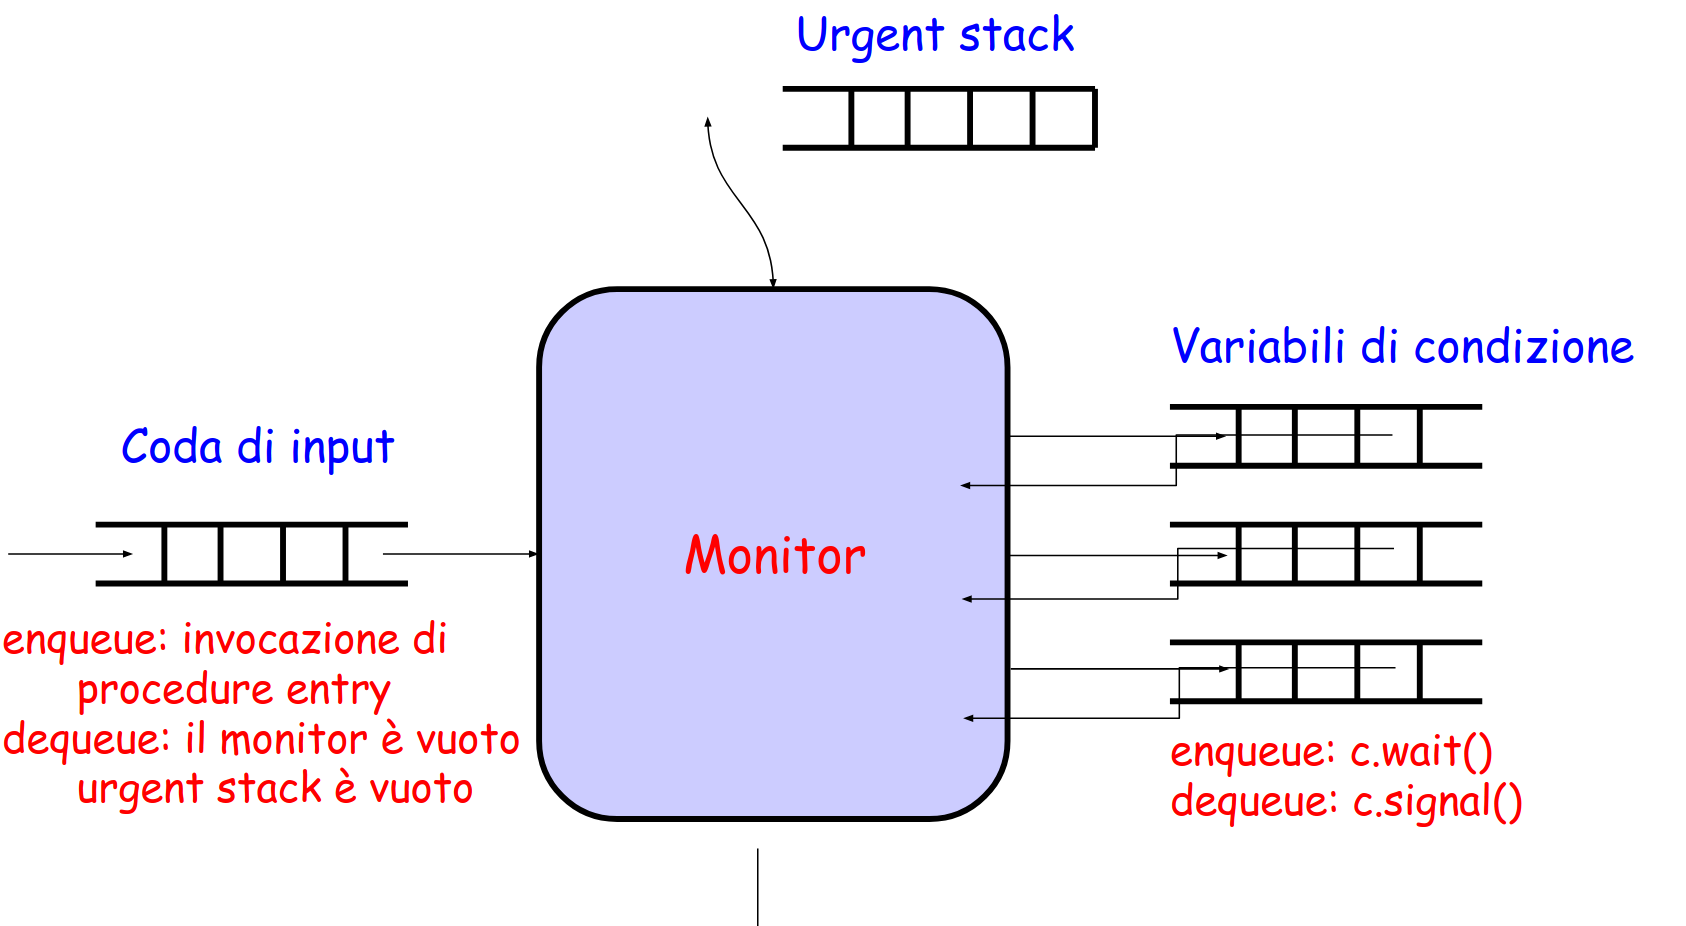
\includegraphics[width=0.7\linewidth]{Images/Screenshot 2025-01-16 at 12-18-56 so-03.1-concorrenza - so-03.1-concorrenza.pdf.png}
\end{figure}

\subsubsection{ wait/signal vs P/V}

A prima vista \textbf{wait e signal} potrebbero sembrare simili alle operazioni sui semafori \textbf{P e V}, ma in verità ci sono differenze sostanziali.

\begin{itemize}
    \item \textbf{signal} non ha alcun effetto se nessun processo sta attendendo la condizione. Mentre \textbf{V} "memorizza" il verificarsi degli eventi.
    \item \textbf{wait} è sempre bloccante, \textbf{P} (se il semaforo ha valore positivo) no.
    \item Il processo risvegliato dalla \textbf{signal} viene eseguito per primo.
\end{itemize}

\subsubsection{Politiche di signaling}
Signal urgent è la politica "classica" di signaling.
SU - signal urgent.

Ne esistono altre..

\subsection{Implementazione dei semafori}

\begin{lstlisting}
monitor Semaphore {
    int value;
    condition c; /* value > 0 */

    procedure entry void P() {
        value--;
        if (value < 0)
            c.wait();
    }

    procedure entry void V() {
        value++;
        c.signal();
    }

    Semaphore(int init) {
        value = init;
    }
}
\end{lstlisting}
\newpage

\subsection{Monitor - R/W}
\begin{lstlisting}
process Reader {
    while (true) {
        rwController.startRead();
        //read the database
        rwController.endRead();
    }
}

process Writer {
    while (true) {
        rwController.startWrite();
        //write the database
        rwController.endWrite();
    }
}
\end{lstlisting}
\newpage
\begin{lstlisting}
monitor RWController
    int nr; /* number of readers */
    int nw; /* number of writers */
    condition okToRead; /* nw == 0 */
    condition okToWrite; /* nr == 0 && nw == 0 */

    procedure entry void startRead() {
        if (nw != 0)
            okToRead.wait();
            nr = nr + 1;

        if (nw == 0) /* always true */
            okToRead.signal();
        
        if (nw == 0 && nr == 0) /* always false */
            okToWrite.signal();
}

    procedure entry void endRead() {
        nr = nr - 1;
        if (nw == 0) /* true but useless */
            okToRead.signal();

        if (nw == 0 && nr == 0)
            okToWrite.signal();
    }

    procedure entry void startWrite() {
        if (!(nr==0 && nw==0))
            okToWrite.wait();
            nw = nw + 1;

        if (nw == 0) /* always true */
            okToRead.signal();

        if (nw == 0 && nr == 0) /* always false */
            okToWrite.signal();
}

    procedure entry void endWrite() {
        nw = nw - 1;
        if (nw == 0) /* Always true */
            okToRead.signal();
        
        if (nw == 0 && nr == 0)
            okToWrite.signal();
        }

    RWController() { /* Constructor */
        nr = nw = 0;
    }

\end{lstlisting}

E' possibile semplificare il codice eliminando le righe if quando sempre vere, eliminando le righe if e il ramo opportuno quando sempre falso.
\newpage
\subsubsection{Monitor - R/W semplificato}
\begin{lstlisting}
    procedure entry void startRead() {
        if (nw != 0) okToRead.wait();
            nr = nr + 1;
            okToRead.signal();
    }

    procedure entry void endRead() {
        nr = nr - 1;
        if (nr == 0) 
            okToWrite.signal();
    }

    procedure entry void startWrite() {
        if (!(nr=0 && nw =0)) 
            okToWrite.wait();
            nw = nw + 1;
    }

    procedure entry void endWrite() {
        nw = nw - 1;
        okToRead.signal();
        if (nw == 0 && nr == 0) 
            okToWrite.signal();
    }
\end{lstlisting}

\subsection{Monitor - Produttore / consumatore}
\begin{lstlisting}
process Producer {
    Object x;
    while (true) {
        x = produce();
        pcController.write(x);
    }
}

process Consumer {
    Object x;
    while (true) {
        x = pcController.read();
        consume(x);
    }
}
\end{lstlisting}
\newpage
\begin{lstlisting}
monitor PCController {
    Object buffer;
    condition empty;
    condition full;
    boolean isFull;

    PCController() {
        isFull=false;
    }


    procedure entry Object read() {
        if (!isFull)
            full.wait();
    
        int retvalue = buffer;
        isFull = false;
        empty.signal();
        return retvalue;
    }

    procedure entry void write(int val) {
        if (isFull)
            empty.wait();
   
        buffer = val;
        isFull = true;
        full.signal();
        }
    }
\end{lstlisting}

\subsection{Monitor - Buffer limitato }
\begin{lstlisting}
monitor PCController {
    Object[] buffer;
    condition okRead, okWrite;
    int count, rear, front;

    PCController(int size) {
        buffer = new Object[size];
        count = rear = front = 0;
    }

    procedure entry Object read() {
        if (count == 0)
            okRead.wait();

        int retval = buffer[rear];
        cont--;
        rear = (rear+1) % buffer.length;
        okWrite.signal();
        return retval;
    }
    
    procedure entry void write(int val) {
        if (count == buffer.length)
            okWrite.wait();
        buffer[front] = val;
        count++;
        front = (front+1) %
        buffer.length;
        okRead.signal();
    }
\end{lstlisting}

\subsection{Monitor - Filosofi a cena (no deadlock)}
\begin{lstlisting}
    process Philo[i] {
        while (true) {
            //think
            chopstick[MIN(i,i+1)].pickup();
            chopstick[MAX(i,i+1)].pickup();
            //eat
            chopstick[MIN(i,i+1)].putdown();
            chopstick[MAX(i,i+1)].putdown();
        }
    }
\end{lstlisting}

\begin{lstlisting}
    monitor DPController {
        condition[] unusedchopstick = new condition[5];
        boolean[] chopstick = new boolean[5];
      
        procedure entry void startEating(int i) {
        
        if (chopstick[i])
            unusedchopstick[i].wait();
            chopstick[i] = true;

        if (chopstick[i+1])
            unusedchopstick[i+1].wait();
            chopstick[i+1] = true;
        }

        procedure entry void finishEating(int i) {
            chopstick[i] = false;
            chopstick[i+1] = false;
            unusedchopstick[i].signal();
            unusedchopstick[i+1].signal();
        }
    }

monitor chopstick[i] {
    boolean inuse = false;
    condition free;
   
    procedure entry void pickup() {
        if (inuse)
            free.wait();
            inuse = true;
    }

    procedure entry void putdown() {
        inuse = false;
        free.signal();
    }
   
\end{lstlisting}    

\newpage

\subsection{Implementazione dei monitor tramite semafori}
\paragraph{Ingredienti:}
\begin{itemize}
    \item un modulo di gestione stack (per urgent)
    \begin{lstlisting}
        interface Stack {
            void push(Object x);
            Object pop();
            boolean empty();
        }
    \end{lstlisting}

    \item un semaforo di mutua esclusione \textbf{e}
    \item per ogni variabile di condizione $cond_i$, una coppia ($c_i$, $nc_i$).
    $c_i$ è un semaforo correlato alla condizione, inizializzato a 0. $nc_i$ è il numero di processi che sono in attesa del verificarsi della condizione.
    \item un "allocatore" di semafori \textit{(o alternativamente un semaforo per ogni processo)}.
\end{itemize}

\begin{lstlisting}
    //Inizializzazione
        Semaphore e = new Semaphore(1);
        Stack stack = new Stack();

    //Entrata nel monitor
        e.P();
    
    //Wait su cond_i
        nc_i++;
        if (!stack.empty()) {
            Semaphore s = stack.pop();
            s.V();
        } else {
            e.V();
        }
        c_i.P();

    //Signal su cond_i
        if (nci > 0) {
            nc_i--;
            ci.V();
            Semaphore s = new Semaphore(0);
            stack.push(s);
            s.P();
            /* free(s) / garbage coll. */
        }

    //Uscita dal monitor
        if (!stack.empty()) {
            Semaphore s = stack.pop();
            s.V();
        } else {
            e.V();
    }
\end{lstlisting}

\newpage
\section{Message passing}
\subsection{Introduzione}
Abbiamo già visto paradigmi di sincronizzazione come: semafori, monitor. In questi paradigmi, la comunicazione avviene tramite memoria condivisa.

I paradigmi di comunicazione come il \textbf{message passing} permettono la comunicazione tra processi tramite messaggi.

La sincronizzazione avviene tramite lo scambio di messaggi, e non più semplici segnali.

\subsubsection{Definizioni}
Un \textbf{messaggio} è un insieme di informazioni formattate da un processo mittente e interpretate da un processo destinatario.

Un meccanismo di "\textbf{scambio di messaggi}" copia le informazioni di un messaggio da uno spazio di indirizzamento
di un processo allo spazio di indirizzamento di un altro processo.
\begin{figure} [h]
    \centering
    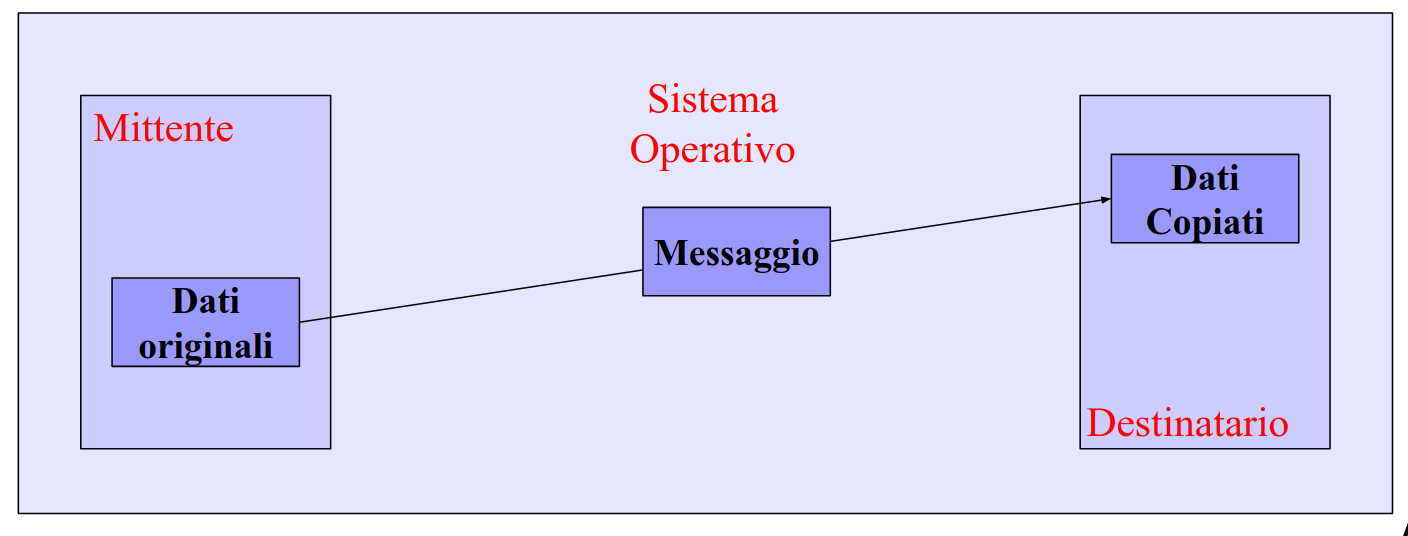
\includegraphics[width=0.7\linewidth]{Images/Screenshot 2025-01-16 at 13-01-13 so-03.1-concorrenza - so-03.1-concorrenza.pdf.png}
\end{figure}

\subsubsection{Operazioni}
\paragraph{send:} utilizzata dal processo mittente per "spedire" un messaggio ad un processo destinatario specificato.
\paragraph{receive:} utilizzata dal processo destinatario per "ricevere" un messaggio da un processo mittente. Il processo mittente può essere specificato, o no.

Il passaggio dallo spazio di indirizzamento del mittente a quello del destinatario è mediato dal sistema operativo (protezione memoria), il processo destinatario deve eseguire un'operazione receive per ricevere qualcosa.

\subsubsection{Tassonomia}
\begin{itemize}
    \item MP sincrono \begin{itemize}
        \item Send sincrono
        \item Receive bloccante
    \end{itemize}
    \item MP asincrono \begin{itemize}
        \item Send asincrono
        \item Receive bloccante
        \end{itemize}
    \item MP completamente asincrono \begin{itemize}
        \item Send asincrono
        \item Receive non bloccante
        \end{itemize}
\end{itemize}

\subsection{MP sincrono}
\subsubsection{Operazione send sincrona}
Sintassi: \lstinline{ssend(m, q)}.

Il mittente p spedisce il messaggio m al processo q, restando bloccato fino a quando q non esegue l'operazione \lstinline{sreceive(m, p)}.

\subsubsection{Operazione receive bloccante}
Sintassi: \lstinline{m = sreceive(p)}

Il destinatario q riceve il messaggio m dal processo p; se il mittente non ha ancora spedito alcun messaggio, il destinatario si blocca in attesa di ricevere un messaggio, è possibile lasciare il mittente non specificato (utilizzando *).


\subsection{MP asincrono}
\subsubsection{Operazione send asincrona}
Sintassi: \lstinline{asend(m, q)}.

il mittente p spedisce il messaggio m al processo q, senza bloccarsi in attesa che il destinatario esegua l'operazione \lstinline{areceive(m, p)}.

\subsubsection{Operazione receive bloccante}
Sintassi: \lstinline{m = areceive(p)}

Il destinatario q riceve il messaggio m dal processo p; se il mittente non ha ancora spedito alcun messaggio, il destinatario si blocca in attesa di ricevere un messaggio, è possibile lasciare il mittente non specificato (utilizzando *).

\subsection{MP completamente asincrono}
\subsubsection{Operazione send asincrona}
Sintassi: \lstinline{asend(m, q)}.

il mittente p spedisce il messaggio m al processo q, senza bloccarsi in attesa che il destinatario esegua l'operazione \lstinline{nb-receive(m, p)}.

\subsubsection{Operazione receive non bloccante}
Sintassi: \lstinline{m = nb-receive(p)}

Il destinatario q riceve il messaggio m dal processo p; se il mittente non ha ancora spedito alcun messaggio, la nb-receive termina ritornando un messaggio "nullo", è possibile lasciare il mittente non specificato (utilizzando *).

\begin{figure} [h]
    \centering
    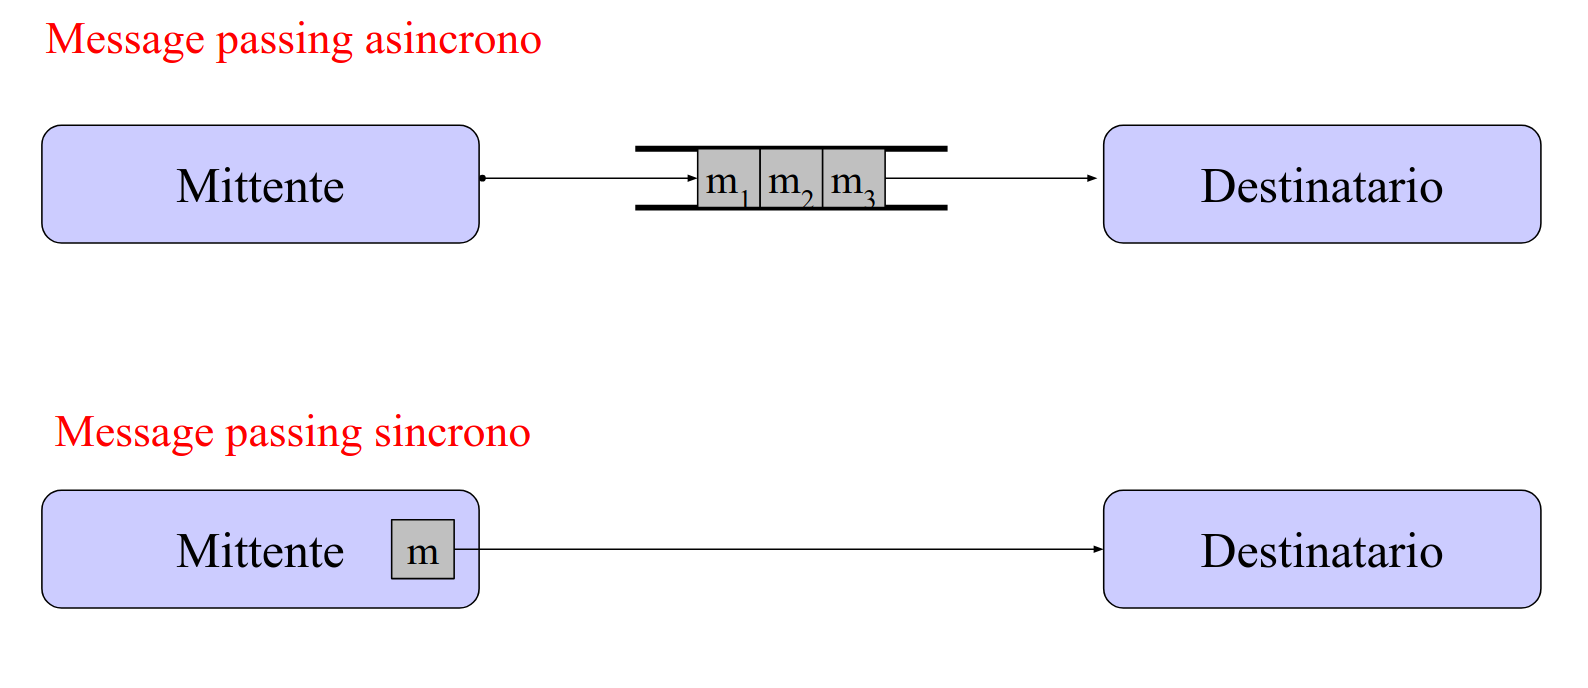
\includegraphics[width=0.7\linewidth]{Images/Screenshot 2025-01-16 at 13-17-46 so-03.1-concorrenza - so-03.1-concorrenza.pdf.png}
\end{figure}

In letteratura ci sono numerose diverse sintassi per descrivere message passing.
Ad esempio, invece che indicare il processo destinazione/mittente, si indica il nome di un canale.

Message passing asincrono con 3 primitive principali: send, receive, reply (Thoth). Non la receive, ma solamente la reply sblocca il mittente, utile per rendere MP simile alle chiamate di procedura remota.
\newpage
\subsection{MP sincrono dato quello asincrono}
\begin{lstlisting}
void ssend(Object msg, Process q) {
    asend(msg, q);
    ack = areceive(q);
}

Object sreceive(p) {
    Object msg = areceive(p);
    asend(ack, p);
    return msg;
}
\end{lstlisting}

\begin{lstlisting}
/* p identifies the calling process */

void asend(Object m, Process q) {
    ssend(SND(m,p,q), server);
}

void areceive(Process q) {
    ssend(RCV(p,q), server);
    Object m = sreceive(server);
    return m;
}

process server {
/* One element x process pair */
    int[][] waiting;
    Queue[][] queue;
    while (true) {
        handleMessage();
    }
}

void handleMessage() {
    msg = sreceive(*);
    if (msg == <SND(m,p,q)>) {
        if (waiting[p,q]>0) {
            ssend(m, p);
            waiting[p,q]--;
        } else {
            queue[p,q].add(m);
        }
    }   else if (msg == <RCV(q,p)>) {
            if (queue[p,q].isEmpty()) {
                waiting[p,q]++;
            } else {
                m = queue[p,q].remove();
                ssend(m, dest);
            }
        }
    }
\end{lstlisting}
\newpage
\subsection{Message Passing - Filosofi a cena}
\begin{lstlisting}
process Philo[i] {
    while (true) {
    //think
    asend(<PICKUP,i>, chopstick[MIN(i, (i+1)%5)]);
    msg = areceive(chopstick[MIN(i, (i+1)%5)]);
    asend(<PICKUP,i>, chopstick[MAX(i, (i+1)%5)]);
    msg = areceive(chopstick[MAX(i, (i+1)%5)]);
    //eat
    asend(<PUTDOWN,i>, chopstick[MIN(i, (i+1)%5)]);
    asend(<PUTDOWN,i>, chopstick[MAX(i, (i+1)%5)]);
    }
}
\end{lstlisting}

\begin{lstlisting}
process chopstick[i] {
    boolean free = true;
    Queue queue = new Queue();
    while (true) {
        handleRequests();
    }
}

void handleRequests() {
    msg = areceive(*);
    if (msg == <PICKUP,j>) {
        if (free) {
            free = false;
            asend(ACK, philo[j]);
        } else {
            queue.add(j);
        }
    } else
        if (msg == <PUTDOWN, j>) {
            if (queue.isEmpty()) {
                free = true;
            } else {
                k = queue.remove();
                asend(ACK, philo[k]);
            }
        }
}
\end{lstlisting}
\newpage
\subsection{Message Passing - Produttori e consumatori}
\begin{lstlisting}
process Producer {
    Object x;
    while (true) {
        x = produce();
        ssend(x, PCmanager);
    }
}

process Consumer{
    Object x;
    while (true) {
        x = sreceive(PCmanager);
        consume(x);
    }
}

process PCmanager {
    Object x;
    while (true) {
        x = sreceive(Producer);
        ssend(x, Consumer);
    }
}
\end{lstlisting}

\section{Conclusioni} 
\subsection{Riassunto}
\begin{itemize}
    \item \textbf{Semafori:} fondamentale primitiva di sincronizzazione, effettivamente offerta dai S.O. . Di livello troppo basso; facile commettere errori.
    \item  \textbf{Monitor:} meccanismi integrati nei linguaggi di programmazione, pochi linguaggi di larga diffusione sono dotati di monitor; unica eccezione Java, con qualche distinguo.
    \item \textbf{Message passing:} da un certo punto di vista, il meccanismo più diffuso. Può essere poco efficiente (copia dati tra spazi di indirizzamento).
\end{itemize}
\subsection{Potere espressivo}
\paragraph{Definizione:} Si dice che il paradigma di programmazione A è espressivo almeno quanto il paradigma di programmazione B (e si scrive $A \ge B$) quando è possibile esprimere ogni programma scritto con B mediante A.

Ovvero, quando è possibile scrivere una libreria che consenta di implementare le chiamate di un paradigma B esprimendole in termini di A si avrà $A \ge B$.
\newline
Si dice che due paradigmi hanno lo stesso potere espressivo se $A \ge B$ e $B \ge A$.

In vari punti di questi lucidi si mostrano delle relazioni tra i vari paradigmi di programmazione mediante funzioni di implementazione.

Si possono tracciare le seguenti classi di paradigmi:
\begin{itemize}
    \item \textbf{Metodi a memoria condivisa:}
    \begin{itemize}
        \item semafori, semafori binari, monitor hanno tutti lo stesso potere espressivo.
        \item dekker e peterson, Test\&Set necessitano di busy waiting.
    \end{itemize}
    
    \item \textbf{Metodi a memoria privata:} message passing asincrono (ha maggiore potere espressivo) e message passing sincrono.
\end{itemize}

\chapter{Risorse}
\newpage

\section{Introduzione}
Un sistema di elaborazione è composto da un insieme di risorse da assegnare ai processi presenti.
I processi competono nell'accesso alle risorse.

\textit{Esempi di risorse: memoria, stampanti, processore, dischi
interfaccia di rete, descrittori di processo...}

\subsection{Classi di risorse}
Le risorse possono essere suddivise in classi, le risorse appartenenti alla stessa classe sono equivalenti.
\textit{Esempi: byte della memoria, stampanti dello stesso tipo, etc.}

Le risorse di una classe vengono dette \textbf{istanze della classe}, il numero di risorse in una classe viene detto \textbf{molteplicità} del tipo di risorsa.

Un processo non può richiedere una specifica risorsa, ma solo una risorsa di una specifica classe. Una richiesta per una classe di risorse può essere soddisfatta da qualsiasi istanza di quel tipo.

\subsubsection{Assegnazione delle risorse}
\paragraph{Risorse ad assegnazione statica}
Avviene al momento della creazione del processo e rimane valida fino alla terminazione.

\textit{Esempi: descrittori di processi, aree di memoria (in alcuni casi)}

\paragraph{Risorse ad assegnazione dinamica}
I processi richiedono le risorse durante la loro esistenza, le utilizzano una volta ottenute e le rilasciano quando non più necessarie.

\textit{Esempi: periferiche di I/O, aree di memoria (in alcuni casi)}

\subsubsection{Tipi di richieste}
\paragraph{Richiesta singola}
Si riferisce a una singola risorsa di una classe definita, è il caso normale.

\paragraph{Richiesta multipla}
Si riferisce a una o più classi, e per ogni classe, ad una o più risorse, deve essere soddisfatta integralmente.

\paragraph{Richiesta bloccante}
Il processo richiedente si sospende se non ottiene immediatamente
l'assegnazione, la richiesta rimane pendente e viene riconsiderata dalla funzione di gestione ad ogni rilascio.

\paragraph{Richiesta non bloccante}
La mancata assegnazione viene notificata al processo richiedente, senza provocare la sospensione.

\subsubsection{Tipi di risorse}

\paragraph{Risorse seriali (o con accesso mutuamente esclusivo)}
Una singola risorsa non può essere assegnata a più processi contemporaneamente.

\textit{Esempi: i processori, le sezioni critiche, le stampanti}

\paragraph{Risorse non seriali}

\textit{Esempio: file di sola lettura}


\paragraph{Definizione:} Una risorsa si dice prerilasciabile se la funzione di gestione può sottrarla ad un processo prima che questo l'abbia effettivamente rilasciata.

\paragraph{Meccanismo di gestione:} Il processo che subisce il prerilascio deve sospendersi, la risorsa prerilasciata sarà successivamente restituita al processo.

Una risorsa è prerilasciabile: se il suo stato non si modifica durante l'utilizzo oppure il suo stato può essere facilmente salvato e ripristinato.

\textit{Esempi: processore, blocchi o partizioni di memoria
(nel caso di assegnazione dinamica)}

\subsection{Risorse non prerilasciabili}

\paragraph{Definizione:} La funzione di gestione non può sottrarle al processo al quale sono assegnate, sono non prerilasciabili le risorse il cui stato non può essere salvato e ripristinato.

\textit{Esempi: stampanti, classi di sezioni critiche, partizioni di memoria (nel caso di gestione statica)}

\section{Deadlock}
Come abbiamo visto i deadlock impediscono ai processi di terminare correttamente, inoltre le risorse bloccate in deadlock non possono essere utilizzati da altri processi.

Vedremo ora le condizioni che necessarie affinché un deadlock si presenti e le tecniche che possono essere utilizzate per gestire  questo problema.

\subsection{Condizioni per avere deadlock}
\begin{itemize}
    \item \textbf{Mutua esclusione:} le risorse coinvolte devono essere seriali
    \item \textbf{Assenza di prerilascio:} le risorse coinvolte non possono essere prerilasciate, ovvero devono essere rilasciate volontariamente dai processi che le controllano
    \item \textbf{Richieste bloccanti (detta anche "hold and wait"):} le richieste devono essere bloccanti, e un processo che ha già ottenuto risorse può chiederne ancora
    \item \textbf{Attesa circolare:} esiste una sequenza di processi $P_0$, $P_1$ , ..., $P _n$, tali per cui $P_0$ attende una risorsa controllata da $P_1$ e $P_1$ attende una risorsa controllata da $P_2$, ..., e $P_n$ attende una risorsa controllata da $P_0$.
\end{itemize}


L'insieme di queste condizioni è necessario e sufficiente. 
Devono valere tutte contemporaneamente affinché un deadlock si presenti nel sistema.

\subsection{Grafo di Holt}

\paragraph{Caratteristiche:} 
\begin{itemize}
    \item è un grafo diretto: gli archi hanno una direzione.
    \item è un grafo bipartito: i nodi sono suddivisi in due sottoinsiemi e non esistono archi che collegano nodi dello stesso sottoinsieme. I sottoinsiemi sono risorse e processi.
    \item gli archi risorsa → processo indicano che la risorsa è assegnata al processo.
    \item gli archi processo → risorsa indicano che il processo ha richiesto la risorsa.
\end{itemize}

\begin{figure}[h]
    \centering
    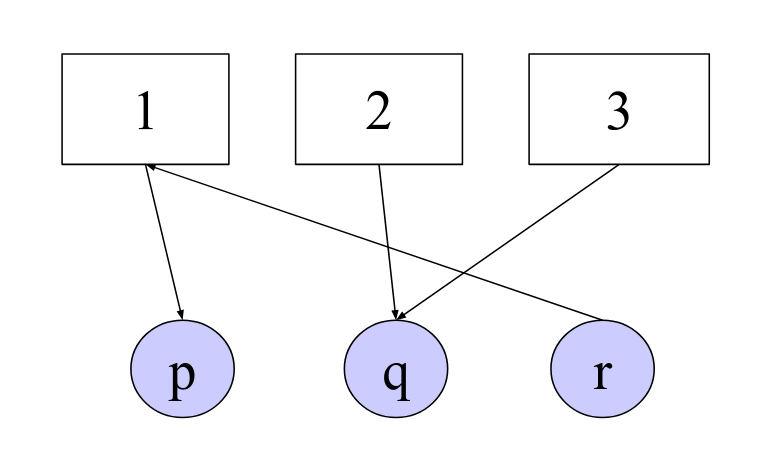
\includegraphics[width=0.4\linewidth]{Images/Screenshot 2024-12-30 at 18-00-42 so-04-risorse - so-04-risorse.pdf.png}
\end{figure}

\subsubsection{Grafo di Holt generale}
Nel caso di classi contenenti più istanze di una risorsa, l'insieme delle risorse è partizionato in classi e gli archi di richiesta sono diretti alla classe e non alla singola risorsa.

\paragraph{Rappresentazione:} i processi sono rappresentati da cerchi, le classi sono rappresentati come contenitori rettangolari
e le risorse come punti all'interno delle classi.

\textit{Nota: non si rappresentano grafi di Holt con archi relativi a richieste che possono essere soddisfatte, se esiste almeno un'istanza libera della risorsa richiesta, la risorsa viene
assegnata.}

\begin{figure} [h]
    \centering
    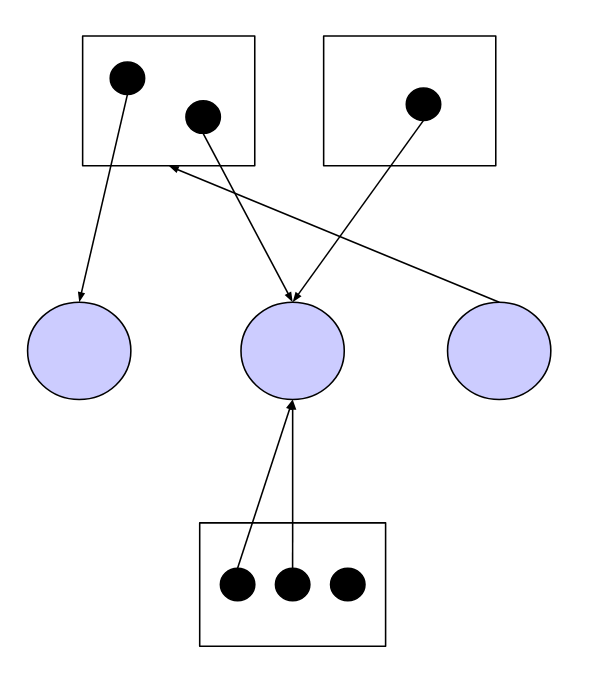
\includegraphics[width=0.2\linewidth]{Images/Screenshot 2024-12-30 at 18-04-17 so-04-risorse - so-04-risorse.pdf.png}
\end{figure}

Alcuni autori preferiscono indicare numericamente:
Sugli archi la molteplicità della richiesta
(archi processo → classe) e la molteplicità dell'assegnazione
(archi classe → processo).
All'interno delle classi il numero di risorse non ancora
assegnate.


\section{Metodi di gestione dei deadlock}

\begin{itemize}
    \item \textbf{Deadlock detection and recovery:} permettere al sistema di entrare in stati di deadlock; utilizzare un algoritmo per rilevare questo stato ed eventualmente eseguire un'azione di recovery.
    \item \textbf{Deadlock prevention / avoidance:} impedire al sistema di entrare in uno stato di deadlock
    \item \textbf{Ostrich algorithm:} ignorare il problema del tutto.
\end{itemize}

\subsection{Deadlock detection}
\paragraph{Descrizione} mantenere aggiornato il grafo di Holt, registrando su di esso tutte le assegnazioni e le richieste di risorse. Utilizzare il grafo di Holt al fine di riconoscere gli stati di deadlock.

\paragraph{Problema:} come riconoscere uno stato di deadlock?

\subsubsection{Caso 1 - Una sola risorsa per classe}

\paragraph{Teorema:} se le risorse sono ad accesso mutualmente esclusivo, seriali e non prerilasciabili, lo stato è di deadlock se e solo se il grafo di Holt contiene un ciclo.

\paragraph{Dimostrazione:} si utilizza una variante del grafo di Holt, detto grafo Wait-For, si ottiene un grafo wait-for eliminando i nodi di tipo risorsa e collassando gli archi appropriati, il grafo di Holt contiene un ciclo se e solo se il grafo Wait-for contiene un ciclo.
Se il grafo Wait-for contiene un ciclo, abbiamo attesa circolare

\begin{figure}[h]
    \centering
    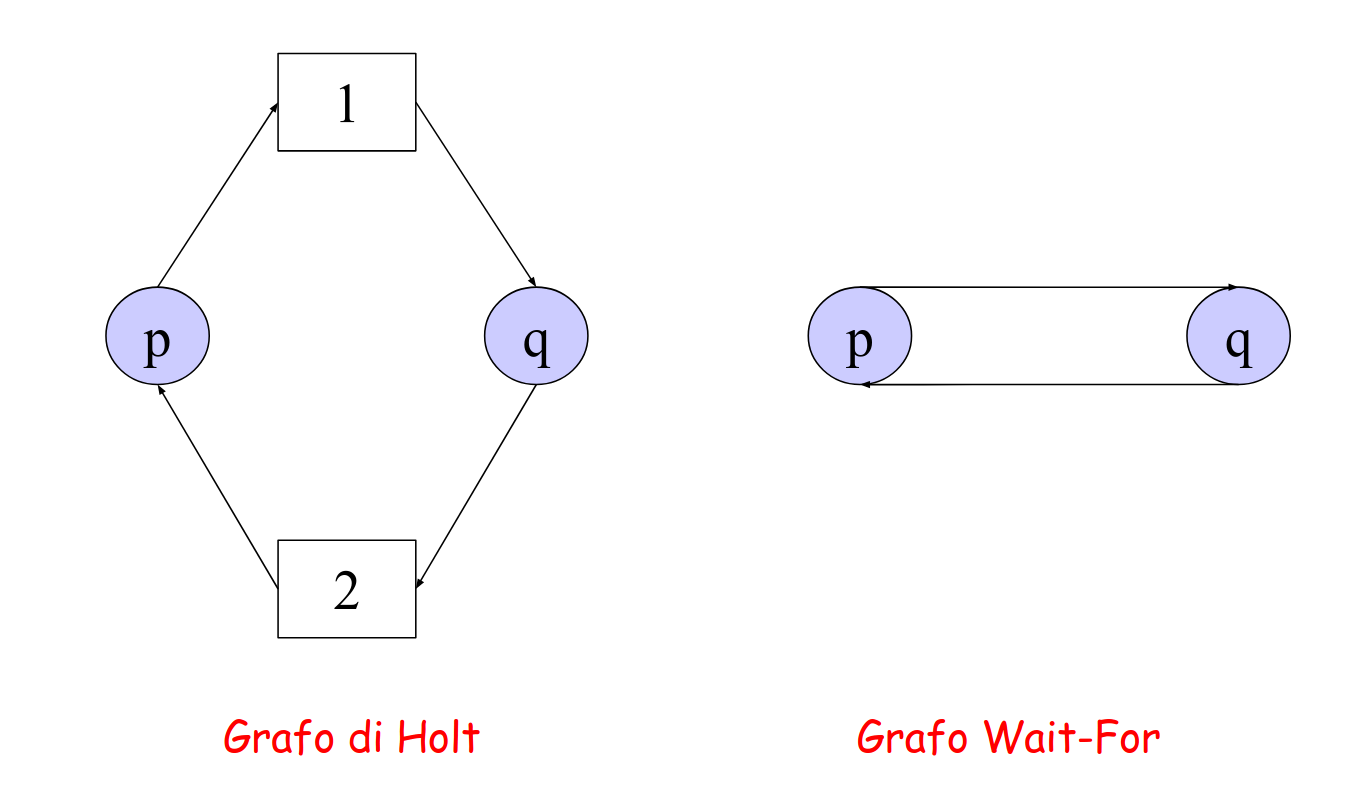
\includegraphics[width=0.4\linewidth]{Images/Screenshot 2024-12-30 at 18-14-14 so-04-risorse - so-04-risorse.pdf.png}
\end{figure}

\subsubsection{Caso 2 - Più risorse per classe}
La presenza di un ciclo nel caso di Holt non è condizione sufficiente per avere deadlock.

\begin{figure} [h]
    \centering
    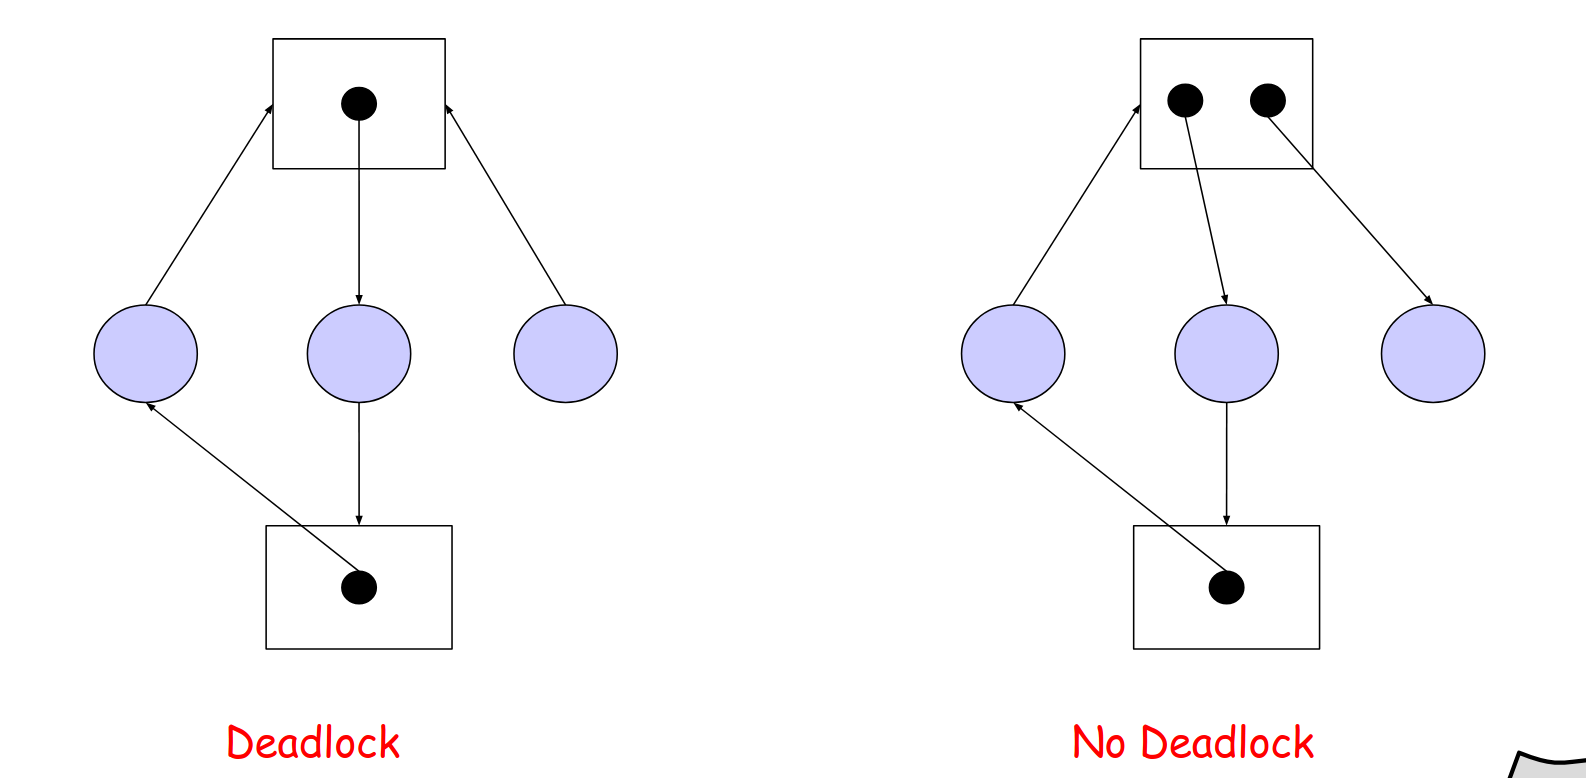
\includegraphics[width=0.5\linewidth]{Images/Screenshot 2024-12-30 at 18-16-02 so-04-risorse - so-04-risorse.pdf.png}
\end{figure}

\subsubsection{Riducibilità di un grafo di Holt}
\paragraph{Definizione:}un grafo di Holt si dice riducibile se esiste almeno un nodo processo con solo archi entranti
\paragraph{Riduzione:} consiste nell'eliminare tutti gli archi di tale nodo e riassegnare le risorse ad altri processi.

\paragraph{Qual è la logica?}eventualmente, un nodo che utilizza una risorsa prima o poi la rilascerà; a quel punto, la risorsa può essere riassegnata.

\begin{figure} [h]
    \centering
    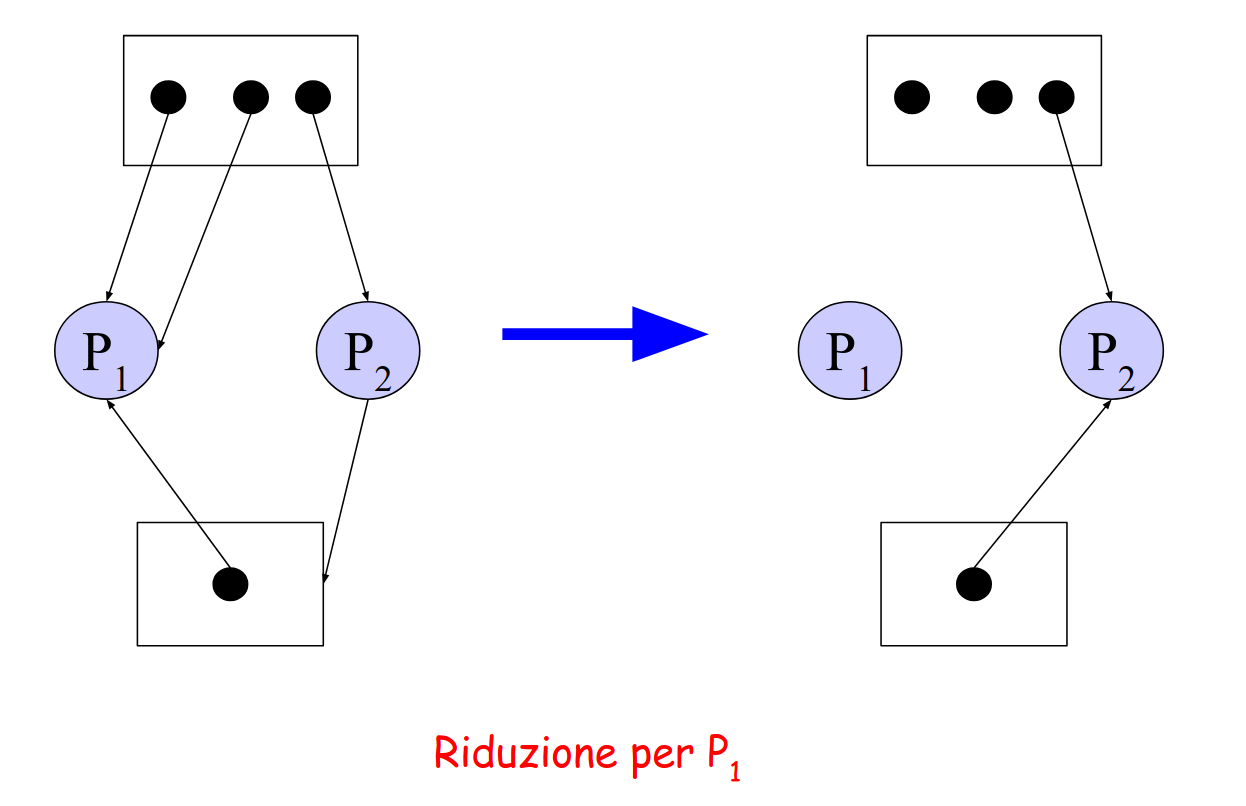
\includegraphics[width=0.5\linewidth]{Images/Screenshot 2024-12-30 at 18-18-35 so-04-risorse - so-04-risorse.pdf.png}
    \caption{Esempio di riduzione}
\end{figure}

\subsubsection{Deadlock detection con grafo di Holt}
\paragraph{Teorema:} se le risorse sono ad accesso mutualmente esclusivo, seriali e non prerilasciabili,  lo stato non è di deadlock se e solo se il grafo di Holt è completamente
riducibile. \textit{(esiste una sequenza di passi di riduzione che elimina tutti gli archi del grafo)}

\subsubsection{Deadlock detection - Knot}

\paragraph{Definizione:} dato un nodo n, l'insieme dei nodi raggiungibili da n viene detto insieme di raggiungibilità di n (scritto \textit{R(n)})

 Un knot del grafo G è il massimo sottoinsieme (non banale) di nodi M tale che per ogni n in M, \textit{R(n)=M}
 
In altre parole: partendo da un qualunque nodo di M, si possono raggiungere tutti i nodi di M e nessun nodo all'infuori di esso.

\begin{figure} [h]
    \centering
    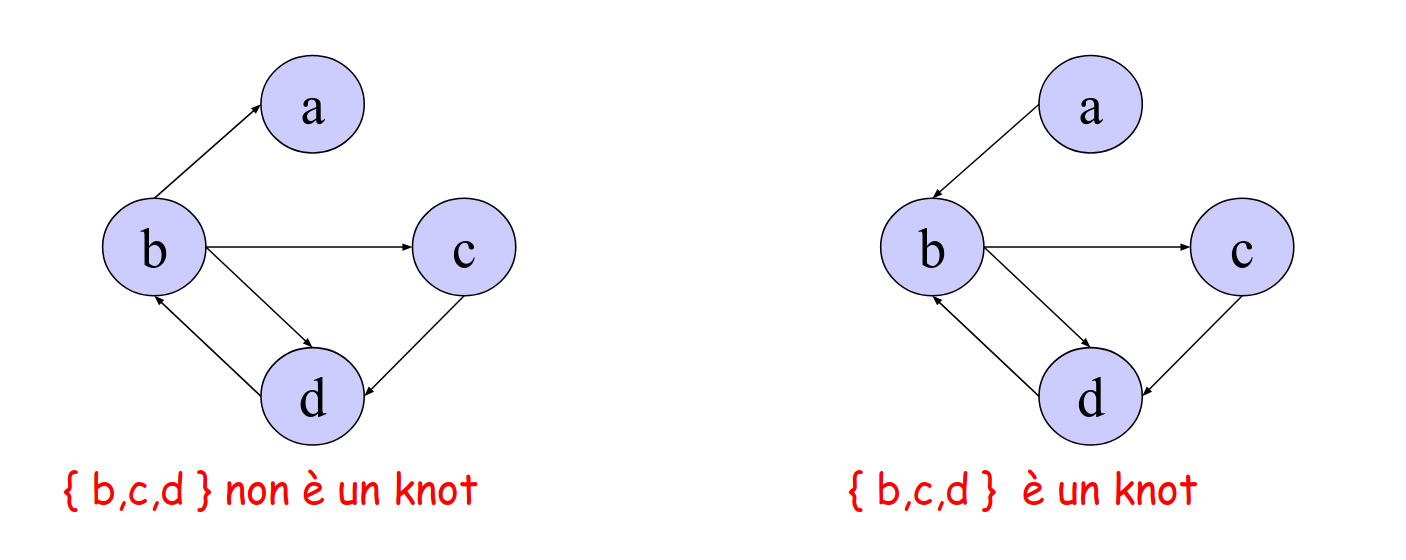
\includegraphics[width=0.6\linewidth]{Images/Screenshot 2025-01-14 at 17-54-33 so-04-risorse - so-04-risorse.pdf.png}
\end{figure}

\paragraph{Teorema:} dato un grafo di Holt con una sola richiesta sospesa per processo
se le risorse sono ad accesso mutualmente esclusivo, seriali e non
prerilasciabili,  allora il grafo rappresenta uno stato di deadlock se e solo se esiste un knot.

\subsection{Deadlock recovery}
Dopo aver rilevato un deadlock bisogna risolvere la situazione.

La soluzione può essere:
\begin{itemize}
    \item \textbf{Manuale:} l'operatore viene informato e eseguirà alcune azioni che permettano al sistema di proseguire.
    \item \textbf{Automatica:} il sistema operativo è dotato di meccanismi che permettono di risolvere in modo automatico la situazione, in base ad alcune politiche
\end{itemize}

\subsubsection{Meccanismi per il deadlock recovery}
\begin{itemize}
    \item Terminazione totale: tutti i processi coinvolti vengono terminati.
    \item Terminazione parziale: viene eliminato un processo alla volta, fino a quando il deadlock non scompare.
    \item Preemption: una risorsa (o più di una, se necessario) viene sottratta ad uno dei processi coinvolti nel deadlock.
    \item Checkpoint/rollback: lo stato dei processi viene periodicamente salvato su disco
(checkpoint). 
In caso di deadlock, si ripristina (rollback) uno o più processi
ad uno stato precedente, fino a quando il deadlock non scompare
\end{itemize}


Terminare processi può essere costoso, questi processi possono essere stati eseguiti per molto tempo; se terminati, dovranno ripartire da capo.
Terminare processi può lasciare le risorse in uno stato inconsistente, se un viene terminato nel mezzo di una sezione critica.

Fare preemption non sempre è possibile, può richiedere interventi manuali.

\subsection{Deadlock prevention e avoidance}
Prevention: per evitare il deadlock si elimina una delle quattro condizioni del deadlock così il deadlock viene eliminato strutturalmente.

Avoidance: prima di assegnare una risorsa ad un processo, si controlla se l'operazione può portare al pericolo di deadlock e in caso, l'operazione viene ritardata.

\subsubsection{Prevention}
Attaccare la condizione di "Mutua esclusione", permettere la condivisione di risorse.

Problemi dello spooling: in generale, lo spooling non sempre è applicabile perchè sposta il problema verso altre risorse.

Attaccare la condizione di "Richiesta bloccante"
\textit{Allocazione totale}, è possibile richiedere che un processo richiede tutte le risorse all'inizio della computazione.
I problemi possono essere: non sempre l'insieme di richieste è noto fin dall'inizio e si riduce il parallelismo.

Attaccare la condizione di "Assenza di prerilascio" non sempre è possibile e può richiedere interventi manuali.

Attaccare la condizione di "Attesa Circolare" \textit{Allocazione gerarchica}, quando alle classi di risorse vengono associati valori di priorità, ogni processo in ogni istante può allocare solamente risorse di priorità superiore a quelle che già possiede.
Se un processo vuole allocare una risorsa a priorità inferiore, deve prima rilasciare tutte le risorse con priorità uguale o superiore a quella desiderata.

L' allocazione gerarchica e allocazione totale danno problemi.
Prevengono il verificarsi di deadlock, ma sono altamente inefficienti perché nell'allocazione gerarchica: l'indisponibilità di una risorsa ad alta priorità ritarda processi che già
detengono risorse ad alta priorità.

Nell'allocazione totale: anche se un processo ha necessità di risorse per poco tempo deve allocarla per tutta la propria esistenza.

\subsubsection{Avoidance - Algoritmo del Banchiere}
Avoidance è l'azione per cui prima di far qualcosa si verifica se porterà a deadlock.

L'algoritmo del banchiere è un algoritmo per evitare lo stallo sviluppato da Dijkstra (1965). 

Il nome deriva dal metodo utilizzato da un ipotetico banchiere di provincia che gestisce un gruppo di clienti a cui ha concesso del credito; non tutti i clienti avranno bisogno dello stesso credito simultaneamente.
\newpage
\section{Algoritmo del Banchiere}
\subsection{Algoritmo del Banchiere Singola valuta}
\paragraph{Descrizione:} 
Un banchiere desidera condividere un capitale (fisso) con un numero
(prefissato) di clienti.

Ogni cliente specifica in anticipo la sua necessità massima di denaro che ovviamente non deve superare il capitale del banchiere.
I clienti fanno due tipi di transazioni: richieste di prestito
e restituzioni.

Il denaro prestato ad ogni cliente non può mai eccedere la necessità massima specificata a priori.

Ogni cliente può fare richieste multiple, fino al massimo importo specificato, una volta che le richieste sono state accolte e il denaro è stato ottenuto deve garantire la restituzione in un tempo finito.

\paragraph{Metodo di funzionamento:} Il banchiere deve essere in ogni istante in grado di soddisfare tutte le richieste dei clienti, o concedendo immediatamente il prestito oppure comunque facendo loro aspettare la disponibilità del denaro in un tempo
finito.

Teniamo conto le seguenti variabili:
\begin{itemize}
    \item $N$ - il numero dei clienti
    \item $IC$ - capitale iniziale
    \item $c_i$ - limite di credito del cliente i ($c_i$ \lt $IC$)
    \item $p_i$ : denaro prestato al cliente i ($p_i \le c_i$ )
    \item $n_i = c_i - p_i$  - credito residuo del cliente i
    \item $SC$ = $IC - \sum_{i=1}^{N}p_i$ -  saldo di cassa 
\end{itemize}

\paragraph{Stato SAFE}
Le richieste che ogni cliente i può fare possono essere soddisfatte dalle risorse attualmente disponibili più tutte le risorse detenute dai processi j soddisfatti precedentemente ($j < i$).
\paragraph{}
Sia s una permutazione dei valori 1...N. \textit{Esempio, con N=4 e s=(1, 3, 4, 2)}

Indichiamo con s(i) l'i-esima posizione della sequenza.

\subparagraph{Si calcoli il vettore \textbf{avail} come segue:}
\begin{itemize}
    \item $avail[1] = SC$
    \item $avail[j+1] = avail[j] + p_{s(j)}$ , con j=1...N-1
\end{itemize}

Uno stato del sistema si dice safe se vale la seguente condizione:
$n_{s(j)} \le avail[j]$ , con j=1...N

\paragraph{Lo stato UNSAFE} è condizione necessaria ma non sufficiente per non avere deadlock. Un sistema in uno stato UNSAFE può evolvere senza procurare alcun deadlock.

\subsubsection{Esempio - stato SAFE} 

\begin{figure}[h]
    \centering
    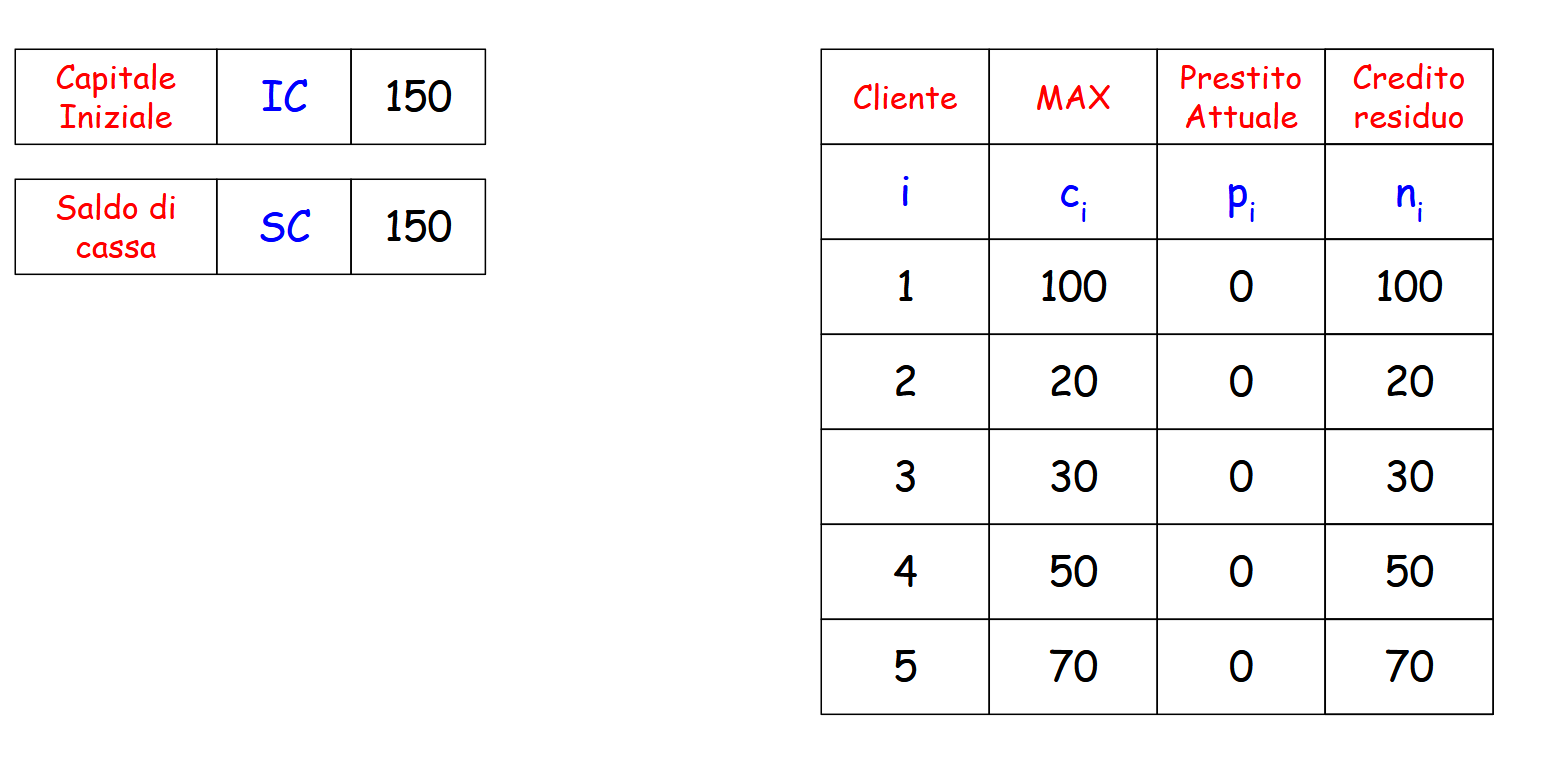
\includegraphics[width=0.7\linewidth]{Images/Screenshot 2025-01-15 113351.png}
    \caption{Situazione iniziale}
\end{figure}

Regola pratica (per il banchiere a singola valuta):
lo stato SAFE può essere verificato usando la sequenza che ordina in modo crescente i valori di $n_i$ (credito residuo di i).

Sono sicuro che concedo ad ogni passo il minimo possibile per poi recuperarlo e aumentare la disponibilità di prestito per il prossimo cliente.
\newpage 

\begin{figure} [h]
    \centering
    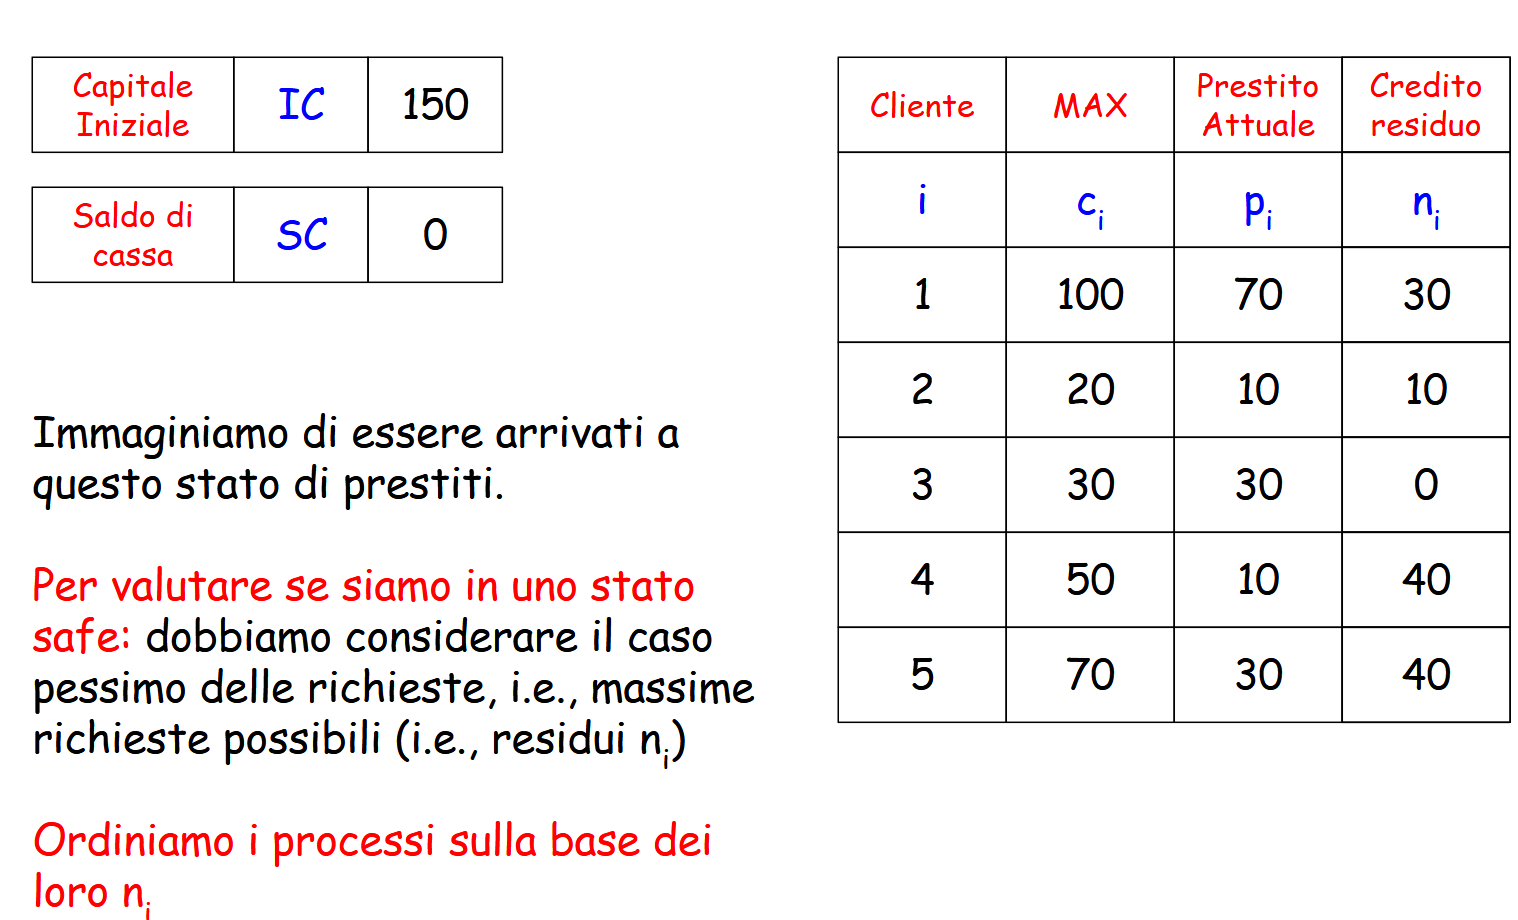
\includegraphics[width=0.7\linewidth]{Images/Screenshot 2025-01-15 113840.png}
\end{figure}

\begin{figure} [h]
    \centering
    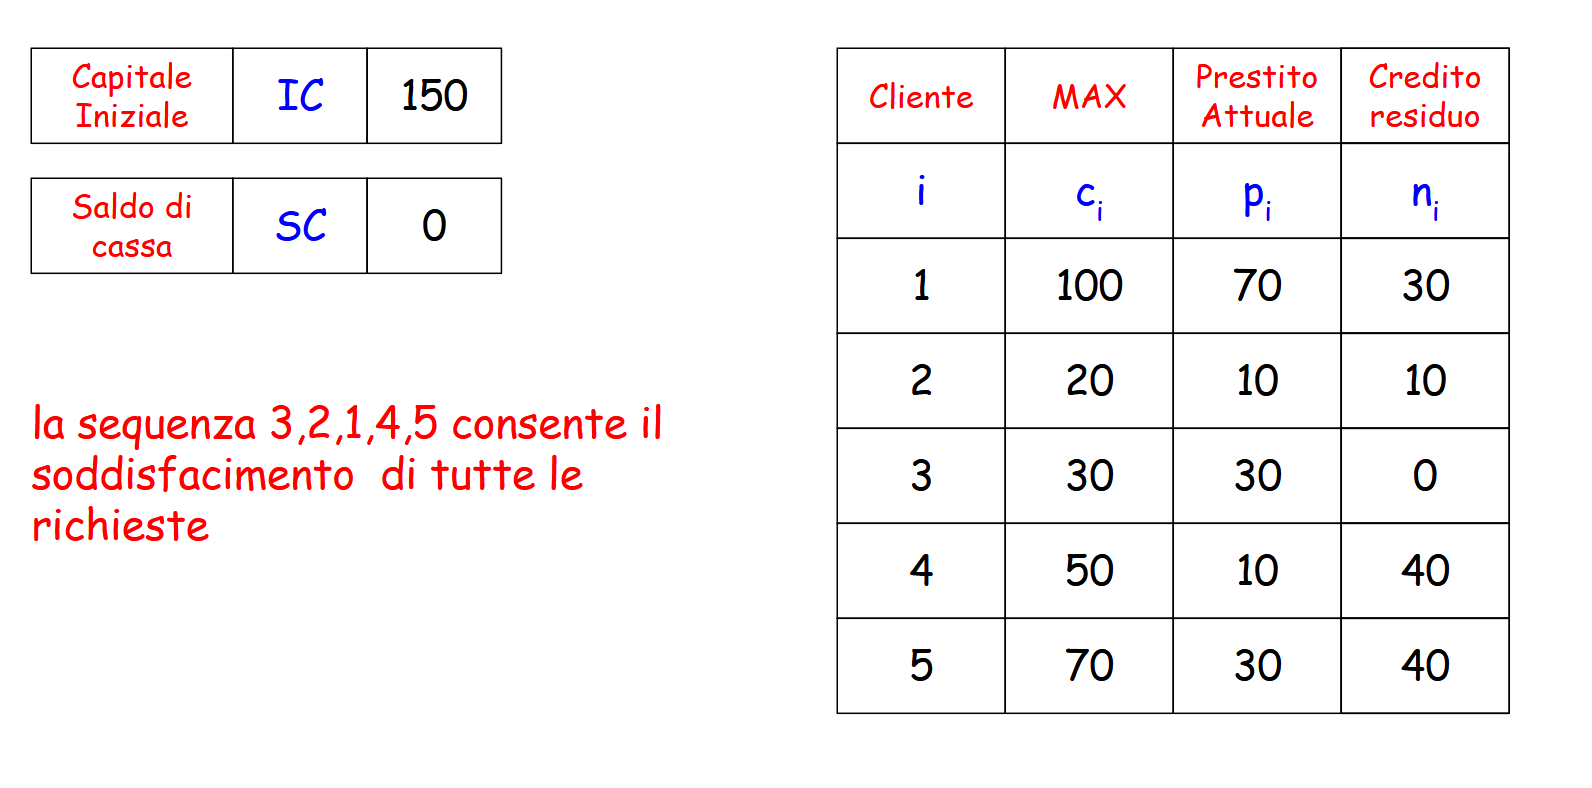
\includegraphics[width=0.7\linewidth]{Images/Screenshot 2025-01-15 114120.png}
\end{figure}

\begin{figure} [h]
    \centering
    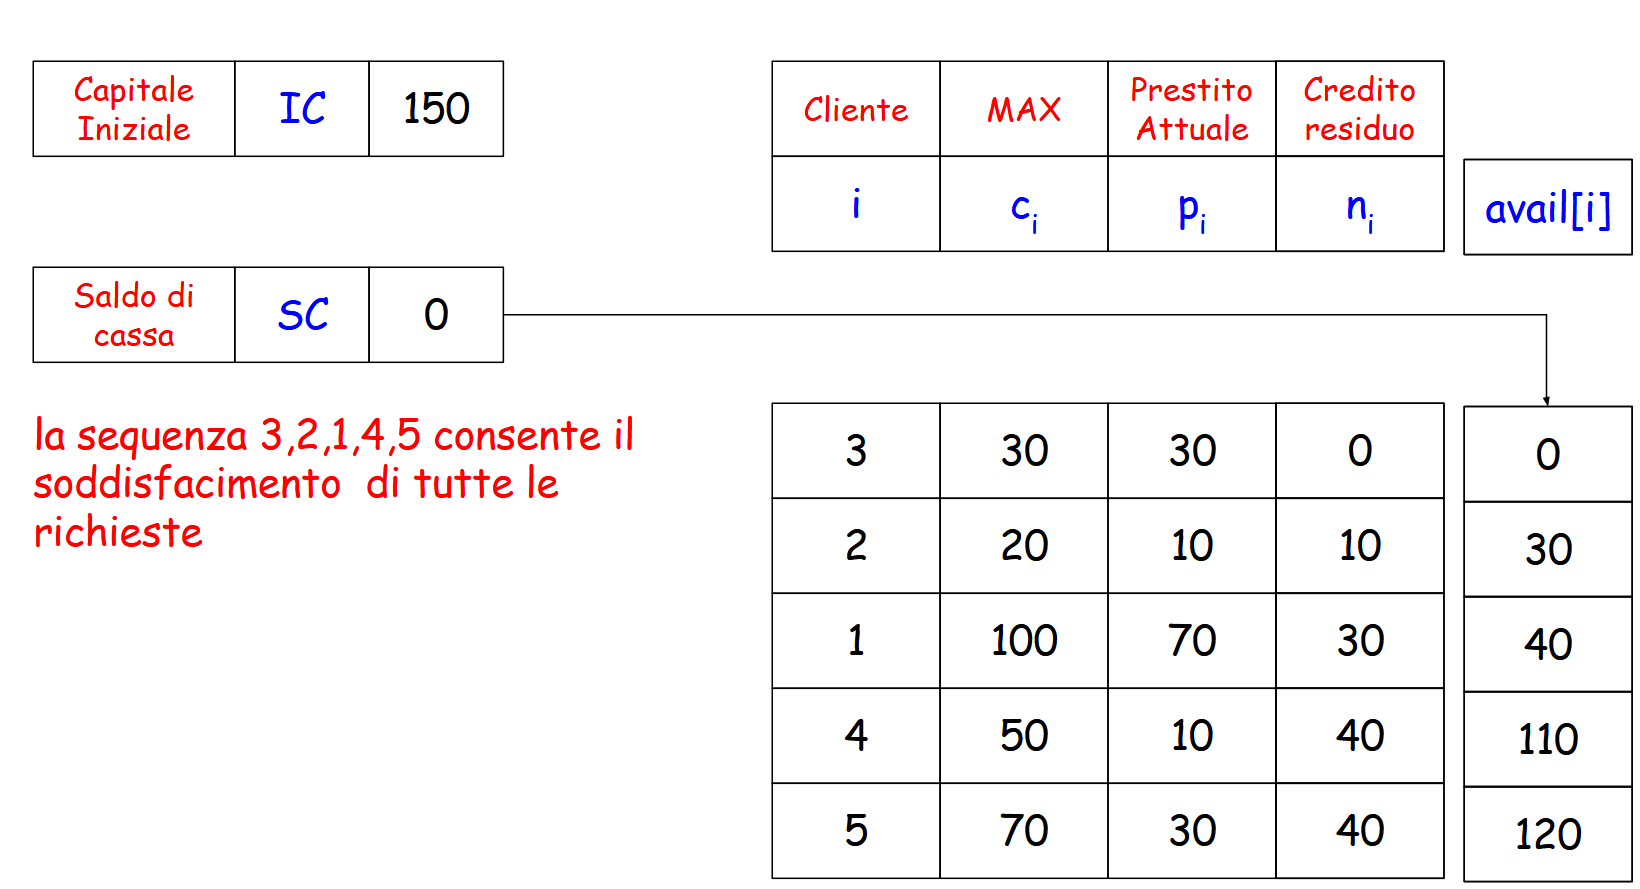
\includegraphics[width=0.7\linewidth]{Images/Screenshot 2025-01-15 114202.png}
\end{figure}

\newpage

\subsubsection{Esempio - stato UNSAFE} 

\begin{figure} [h]
    \centering
    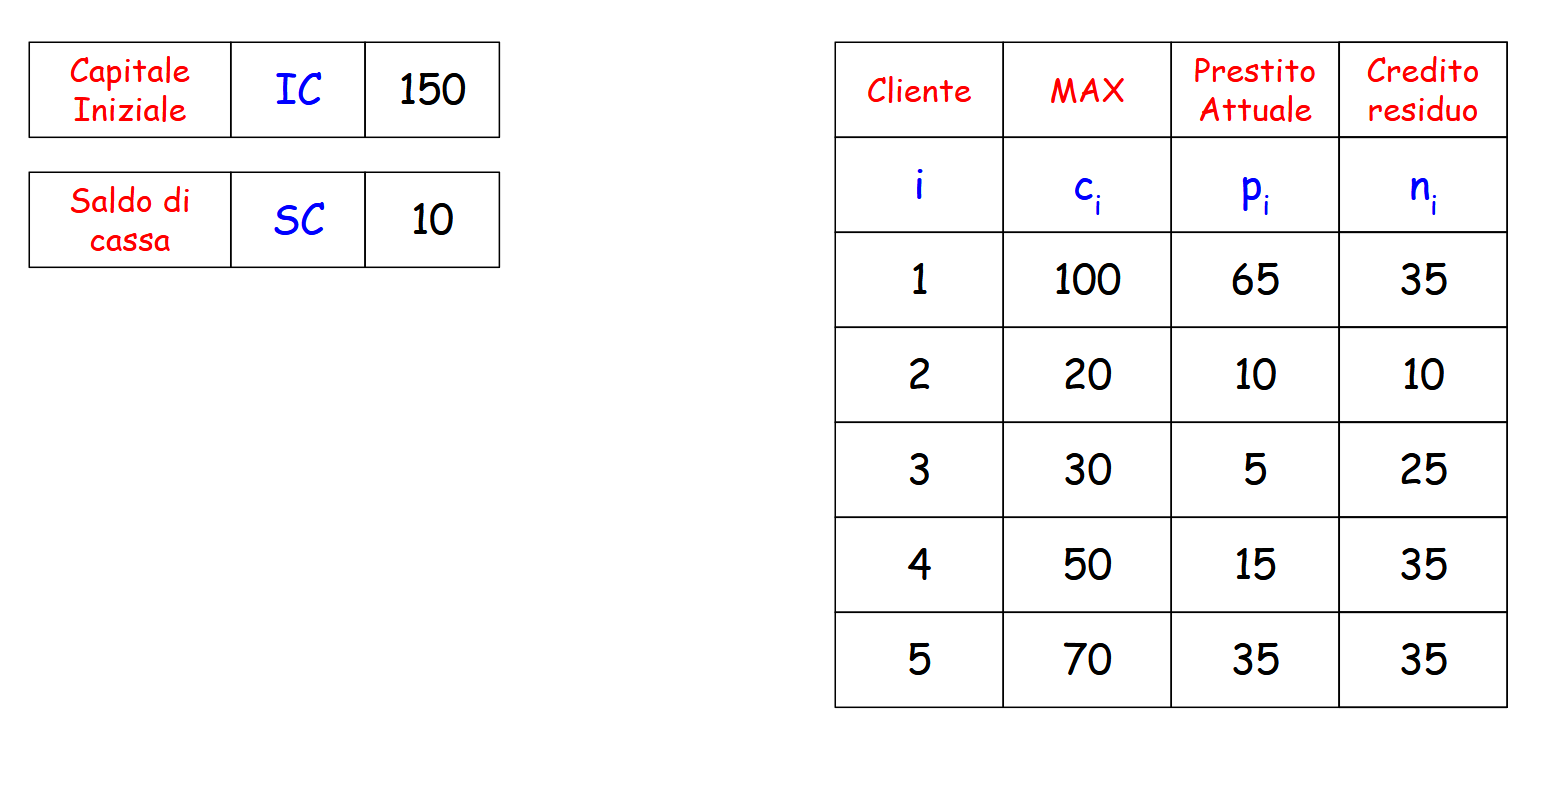
\includegraphics[width=0.7\linewidth]{Images/Screenshot 2025-01-15 114320.png}
\end{figure}

\begin{figure} [h]
    \centering
    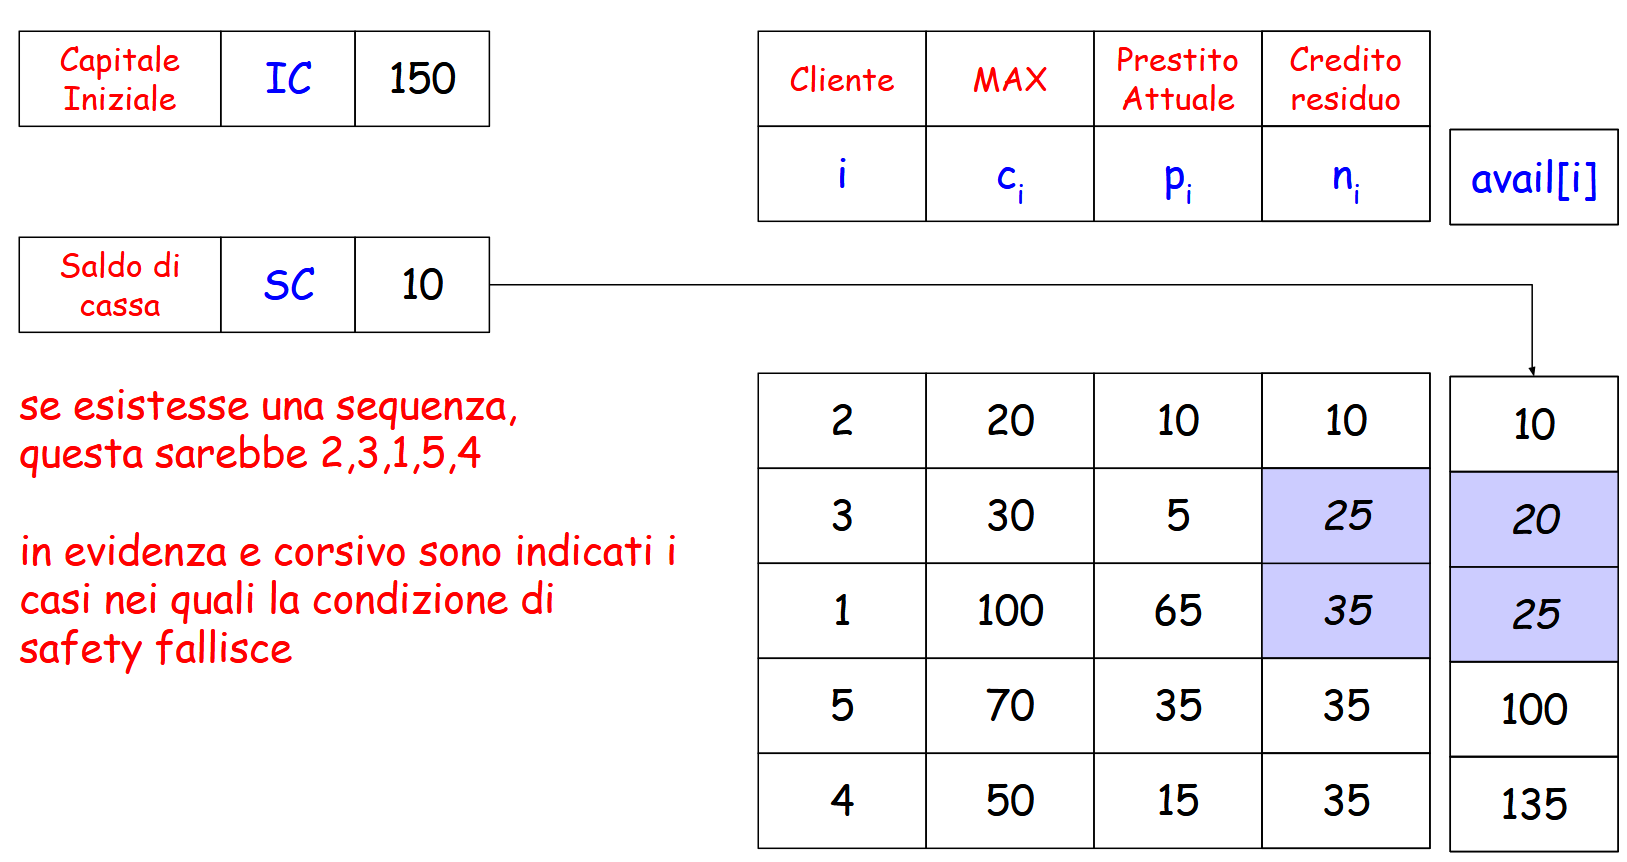
\includegraphics[width=0.7\linewidth]{Images/Screenshot 2025-01-15 114534.png}
\end{figure}

\begin{figure} [h]
    \centering
    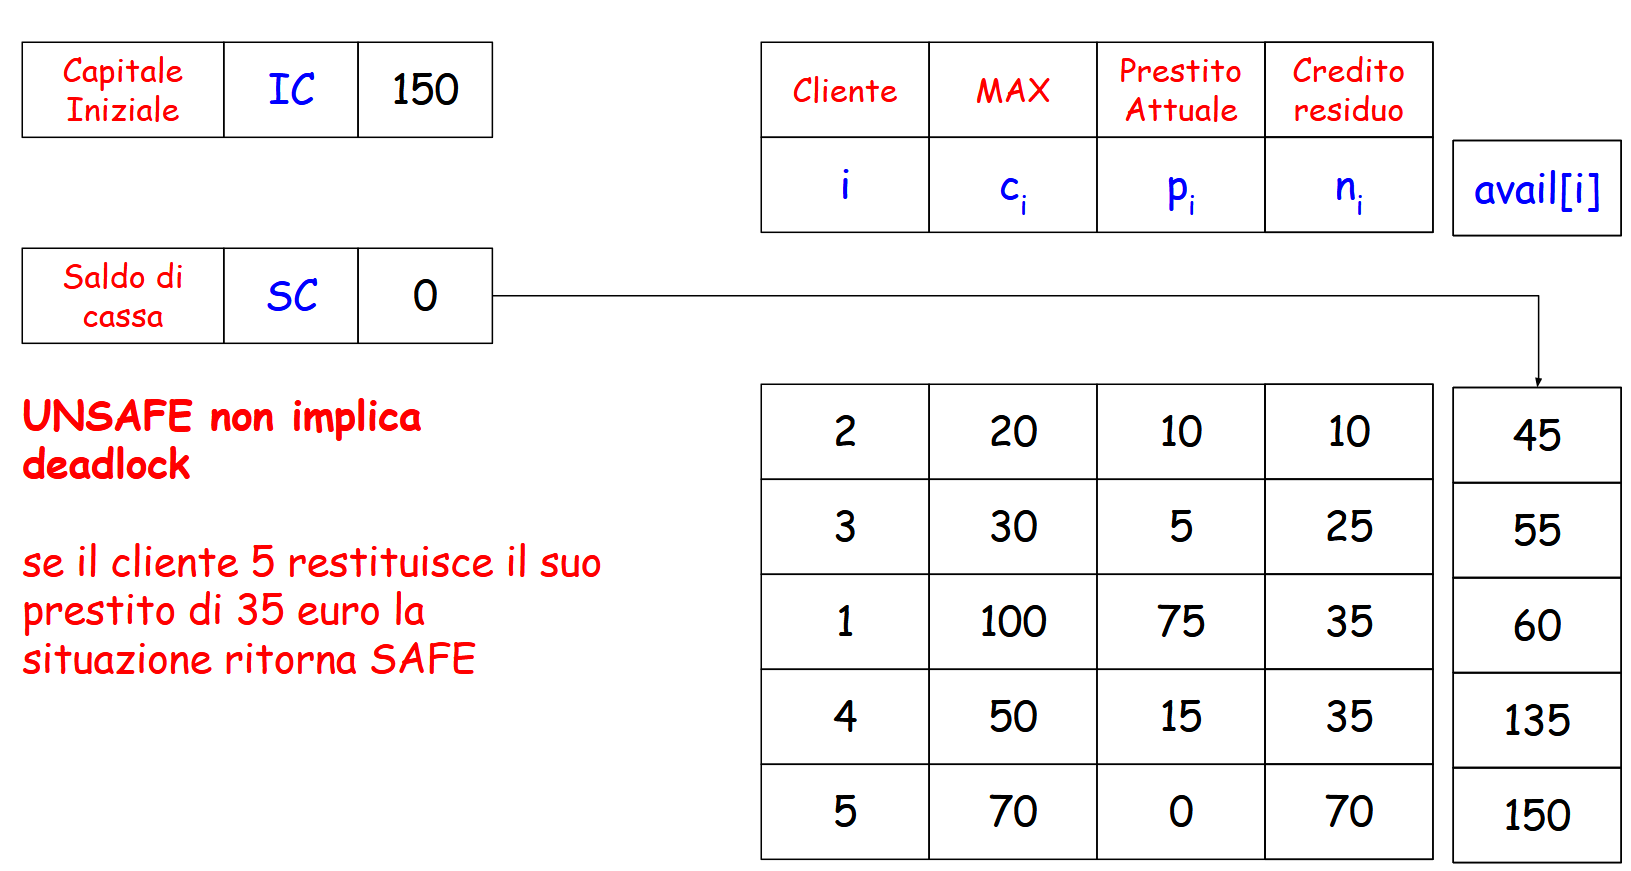
\includegraphics[width=0.7\linewidth]{Images/Screenshot 2025-01-15 114907.png}
\end{figure}

\subsubsection{Conclusione Algoritmo Banchiere singola valuta}
La similitudine fra banchieri e sistemi operativi ora è chiara: il denaro sono le risorse, il sistema le deve allocare ai processi senza che si possa verificare deadlock.

Le definizioni viste fino a questo punto riguardano il caso teorico elementare di un sistema avente un'unica classe di risorse.
\newpage
\subsection{Algoritmo del Banchiere Multivaluta}
L'estensione del problema del banchiere singola valuta dove si ipotizza che il banchiere debba fare prestiti usando valute diverse (euro, dollari, yen, etc.)
Le diverse valute rappresentano diverse classi di risorse.

Teniamo conto le seguenti variabili:
\begin{itemize}
    \item $N$ - il numero dei clienti
    \item $IC_k$ - capitale iniziale della valuta k
    \item $c_{i,k}$ - limite di credito in valuta k del cliente i ($c_{i,k} < IC_k$)
    \item $p_{i,k}$ - denaro prestato in valuta k al cliente i ($p_i,k \le c_{i,k}$)
    \item $n_{i,k} =c_{i,k} - p_{i,k}$ - credito residuo in valuta k del cliente i
    \item $SC_k = IC - \sum_{i=1}^{N} p_{i,k}$ - saldo di cassa in valuta k 
\end{itemize}

\paragraph{Stato SAFE}

Sia s una permutazione dei valori 1...N. Esempio, con N=4 e s=(1, 3, 4, 2).
Indichiamo con s(i) l'i-esima posizione della sequenza.
\subparagraph{Si calcoli il vettore $avail_k$ come segue:}
\begin{itemize}
    \item $avail_k[1] = SC_k$
    \item $avail_k[j+1] = avail_k[j] + p_{s(j)}$ , con j=1...N-1
\end{itemize}

Uno stato del sistema si dice safe se vale la seguente condizione: $n_{s(j),k} \le avail_k[j]$ , con j=1...N

\paragraph{Problema} La regola di ordinare i processi secondo i valori di n i non è applicabile, l'ordine può essere in generale diverso fra le diverse valute gestite dal banchiere.
\paragraph{Soluzione}Si può creare la sequenza procedendo passo passo aggiungendo un processo a caso fra quelli completamente soddisfacibili. Ovvero, al passo j si sceglie quelli per cui: $n_{s(j),k} \le avail_k[j]$

\subsubsection{Esempio - Banchiere Multivaluta}

\begin{figure} [h]
    \centering
    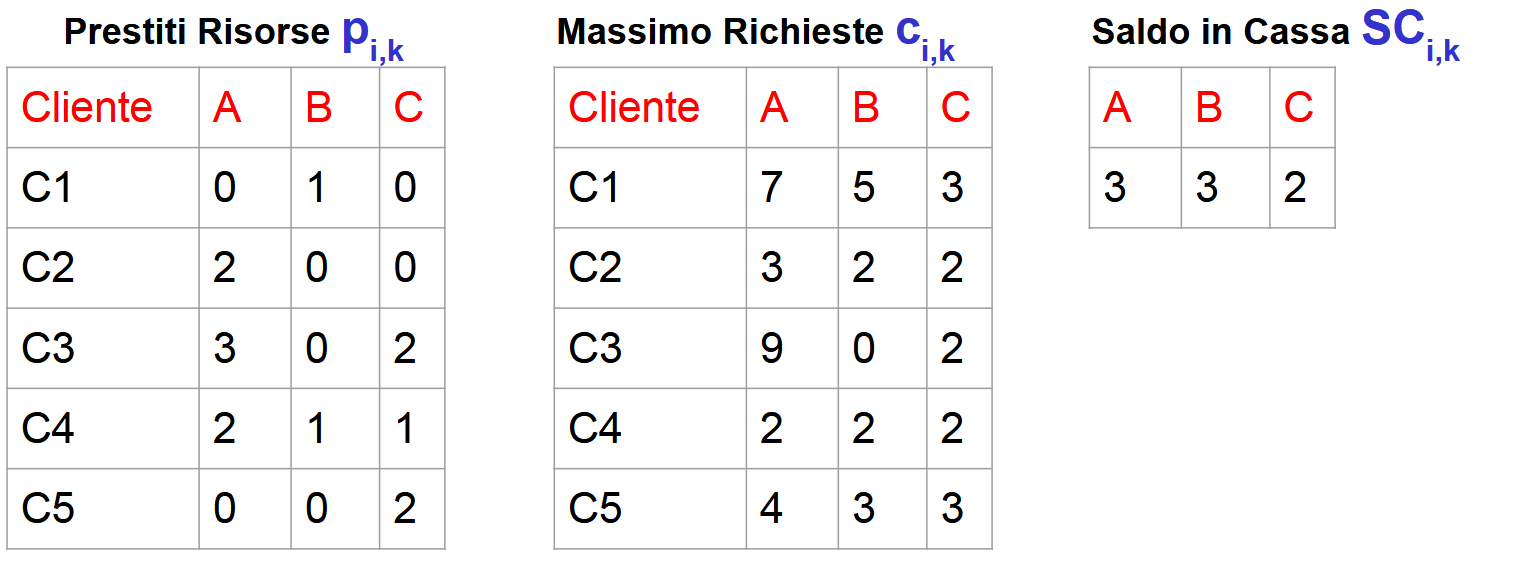
\includegraphics[width=0.65\linewidth]{Images/Screenshot 2025-01-15 122610.png}
\end{figure}

\begin{figure} [h]
    \centering
    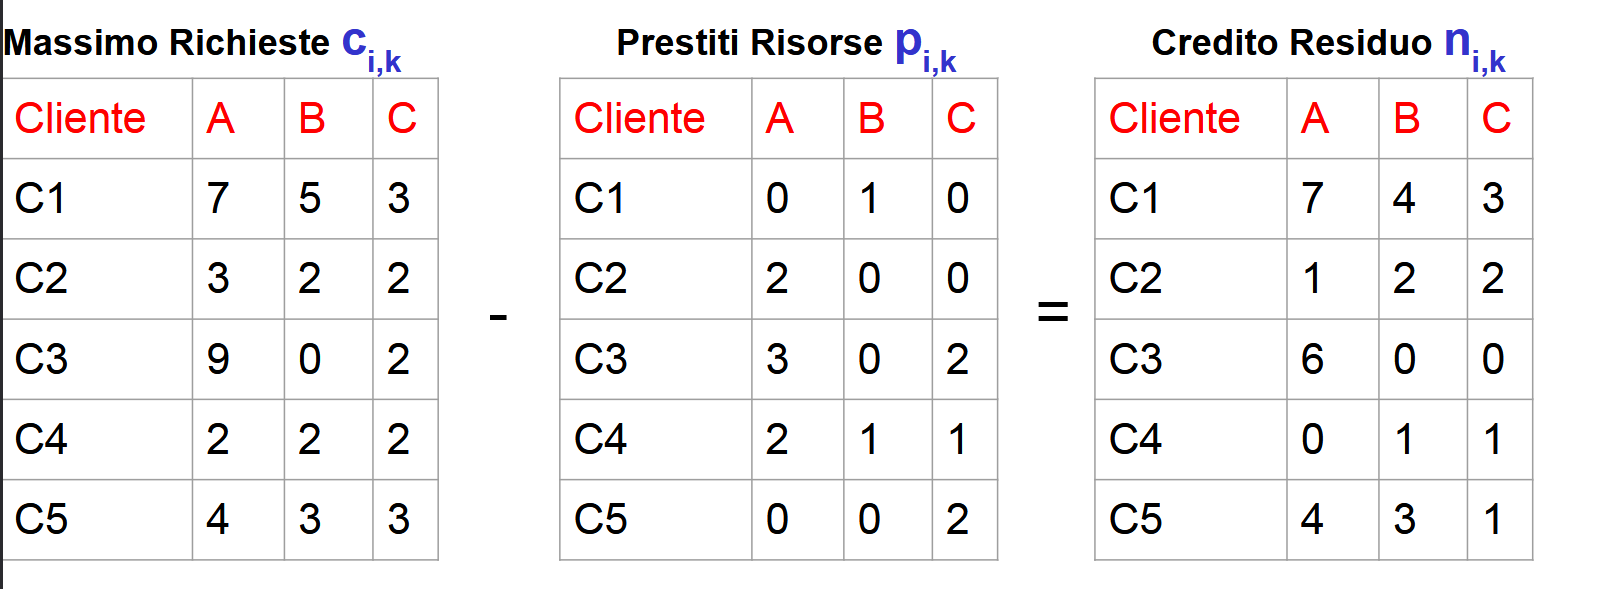
\includegraphics[width=0.65\linewidth]{Images/Screenshot 2025-01-15 122705.png}
\end{figure}

\begin{figure} [h]
    \centering
    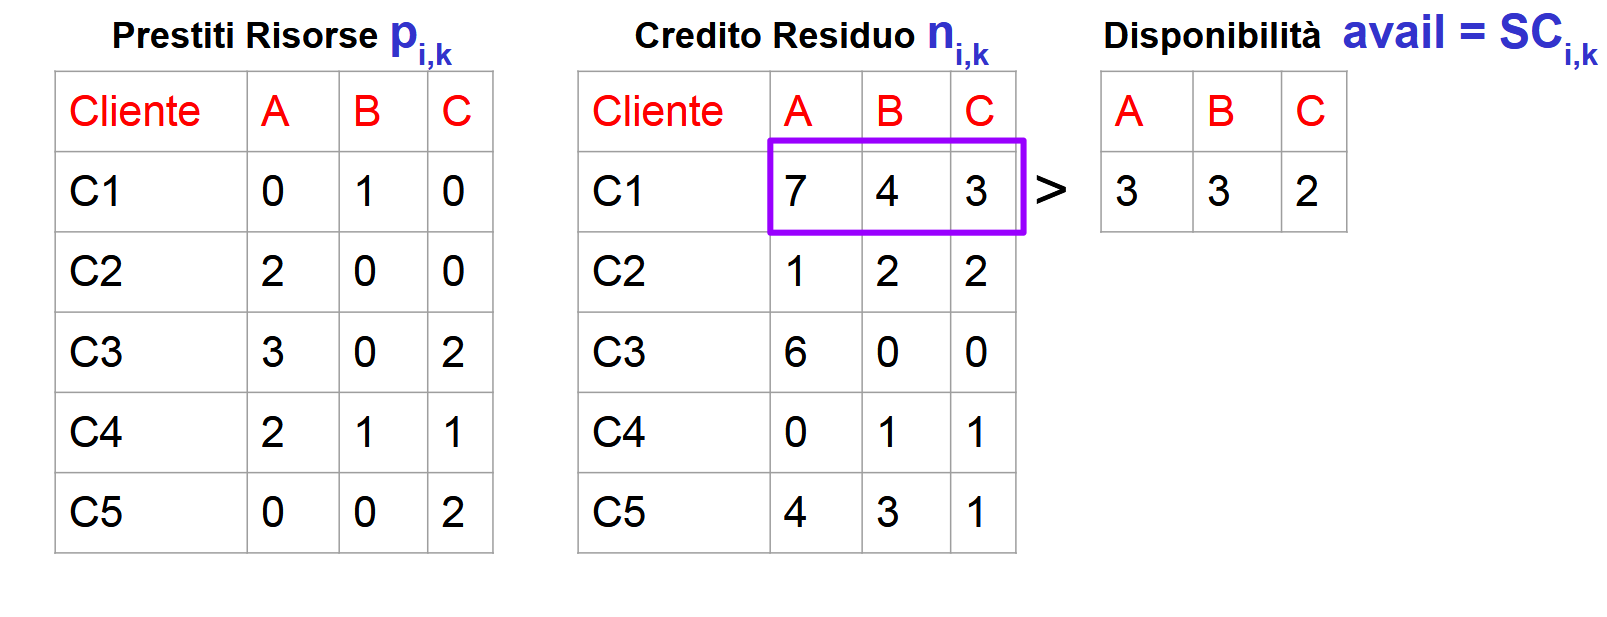
\includegraphics[width=0.65\linewidth]{Images/Screenshot 2025-01-15 122853.png}
\end{figure}

\begin{figure} [h]
    \centering
    \includegraphics[width=0.65\linewidth]{Images/Screenshot 2025-01-15 123110.png}
\end{figure}

\begin{figure} [h]
    \centering
    \includegraphics[width=0.65\linewidth]{Images/Screenshot 2025-01-15 125005.png}
\end{figure}

\begin{figure} [h]
    \centering
    \includegraphics[width=0.65\linewidth]{Images/Screenshot 2025-01-15 125124.png}
\end{figure}

\begin{figure} [h]
    \centering
    \includegraphics[width=0.65\linewidth]{Images/Screenshot 2025-01-15 125217.png}
\end{figure}

\begin{figure} [h]
    \centering
    \includegraphics[width=0.65\linewidth]{Images/Screenshot 2025-01-15 125252.png}
\end{figure}

\begin{figure} [h]
    \centering
    \includegraphics[width=0.65\linewidth]{Images/Screenshot 2025-01-15 125344.png}
\end{figure}

\begin{figure} [h]
    \centering
    \includegraphics[width=0.65\linewidth]{Images/Screenshot 2025-01-15 125412.png}
\end{figure}

\chapter{Memoria}
\newpage

\section{Binding, loading, linking}

La parte del sistema operativo che gestisce la memoria principale si chiama \textbf{memory manager} che in alcuni casi,può gestire anche parte della memoria secondaria, al fine di emulare memoria principale.
I compiti di un memory manager sono: tenere traccia della memoria libera e occupata e allocare memoria ai processi e deallocarla quando non più necessaria.

\subsection{Binding}
\paragraph{Definizione:} con il termine binding si indica l'associazione di indirizzi di memoria ai dati e
alle istruzioni di un programma. Il binding può avvenire durante la compilazione, il caricamento o l'esecuzione.

\subsubsection{Binding durante la compilazione}
Gli indirizzi vengono calcolati al momento della compilazione e resteranno gli stessi ad ogni esecuzione del programma, il codice generato viene detto codice \textbf{assoluto}.
\textit{Esempi: codice per microcontrollori, per il kernel, file COM in MS-DOS}

\begin{figure} [h]
    \centering
    \includegraphics[width=0.7\linewidth]{Images/Screenshot 2025-01-16 at 18-28-27 so-05-memoria - so-05-memoria.pdf.png}
\end{figure}


\paragraph{Vantaggi:} non richiede hardware speciale, è semplice, molto veloce.
\paragraph{Svantaggi:} non funziona con la multiprogrammazione.

\subsubsection{Binding durante il caricamento}
Il codice generato dal compilatore non contiene indirizzi assoluti ma relativi (al PC oppure ad un indirizzo base), questo tipo di codice viene detto \textbf{rilocabile}.
Durante il caricamento il loader si preoccupa di aggiornare tutti i riferimenti agli indirizzi di memoria coerentemente al punto iniziale di caricamento.
\begin{figure} [h]
    \centering
    \includegraphics[width=0.7\linewidth]{Images/Screenshot 2025-01-16 at 18-30-35 so-05-memoria - so-05-memoria.pdf.png}
\end{figure}

\paragraph{Vantaggi:} permette di gestire multiprogrammazione, non richiede uso di hardware particolare.
\paragraph{Svantaggi:} richiede una traduzione degli indirizzi da parte del loader, e quindi formati particolari dei file eseguibili.

\subsubsection{Binding durante l'esecuzione}
L'individuazione dell'indirizzo di memoria effettivo viene effettuata durante l'esecuzione da un componente hardware apposito:
la memory management unit (\textbf{MMU}).

\begin{figure} [h]
    \centering
    \includegraphics[width=0.7\linewidth]{Images/Screenshot 2025-01-16 at 18-33-56 so-05-memoria - so-05-memoria.pdf.png}
\end{figure}

\subsubsection{Indirizzi logici e indirizzi fisici}

\paragraph{Spazio di indirizzamento logico} ogni processo è associato ad uno spazio di indirizzamento logico, gli indirizzi usati in un processo sono indirizzi logici, ovvero riferimenti a
questo spazio di indirizzamento.

\paragraph{Spazio di indirizzamento fisico} ad ogni indirizzo logico corrisponde un indirizzo fisico, la MMU opera come una funzione di traduzione da indirizzi logici a indirizzi fisici.

\begin{figure} [h]
    \centering
    \includegraphics[width=0.25\linewidth]{Images/Screenshot 2025-01-16 at 18-40-39 so-05-memoria - so-05-memoria.pdf.png}
\end{figure}

\subsection{Loading Dinamico}
Il loading dinamico consente di poter caricare alcune routine di libreria solo quando vengono richiamate.
Tutte le routine a caricamento dinamico risiedono su un disco (codice rilocabile), quando servono vengono caricate, le routine poco utili \textit{(e.g., casi di errore rari...)} non vengono caricate in
memoria al caricamento dell'applicazione.

\textit{Nota: spetta al programmatore sfruttare questa possibilità, dato che il sistema operativo fornisce semplicemente una libreria che implementa le funzioni di caricamento dinamico.}


\subsection{Linking statico}
Se il linker collega e risolve tutti i riferimenti dei programmi, le routine di libreria vengono copiate in ogni programma che le usa
\textit{(e.g. printf in tutti i programmi C)}.

\subsection{Linking dinamico}
E' possibile posticipare il linking delle routine di libreria al momento del primo riferimento durante l'esecuzione.
Consente di avere eseguibili più compatti e le librerie vengono implementate come codice reentrant, ovvero esiste una sola istanza della libreria in memoria e tutti i programmi eseguono il codice di questa istanza.

\paragraph{Vantaggi:} risparmio di memoria, consente l'aggiornamento automatico delle versioni delle librerie
che vengono caricate alla successiva attivazione dei programmi.

\paragraph{Svantaggi:} può causare problemi di 'versioning', ovvero conflitti che si verificano quando diverse applicazioni richiedono versioni diverse della stessa libreria condivisa o quando l'aggiornamento di una libreria la rende incompatibile con alcune applicazioni che la utilizzano.
\newpage
\section{Allocazione}
\subsection{Definizioni}
E' una delle funzioni principali del gestore di memoria.
Consiste nel reperire ed assegnare uno spazio di memoria fisica  a un programma che viene attivato, oppure per soddisfare ulteriori richieste effettuate dai programmi durante la loro esecuzione.

\paragraph{Allocazione contigua} tutto lo spazio assegnato ad un programma deve essere formato da celle consecutive.
\paragraph{Allocazione non contigua} è possibile assegnare a un programma aree di memorie separate.

\textit{Nota: la MMU deve essere in grado di gestire la conversione degli indirizzi in modo coerente. Esempio: la MMU basata su rilocazione gestisce solo allocazione contigua.}

\paragraph{Allocazione statica:} un programma deve mantenere la propria area di memoria dal caricamento alla terminazione. Non è possibile rilocare il programma durante l'esecuzione.
\paragraph{Allocazione dinamica:} durante l'esecuzione, un programma può essere spostato all'interno della memoria.

\subsection{Allocazione a partizioni fisse}
\paragraph{Descrizione:} la memoria disponibile (quella non occupata dal s.o.) viene suddivisa in partizioni, ogni processo viene caricato in una delle partizioni libere che ha dimensione sufficiente a contenerlo.

\paragraph{Caratteristiche:} statica e contigua. Molto semplice.
Ma produce spreco di memoria e ha un grado di parallelismo limitato dal numero di partizioni.

\begin{figure} [h]
    \centering
    \includegraphics[width=0.3\linewidth]{Images/Screenshot 2025-01-16 at 19-02-29 so-05-memoria - so-05-memoria.pdf.png}
\end{figure}

E' possibile utilizzare una coda per partizione, oppure una coda
comune per tutte le partizioni. Esiste una sola partizione,
dove viene caricato un unico programma utente.

\subsubsection{Frammentazione interna}
Nell'allocazione a partizione fisse se un processo occupa una dimensione inferiore a quella della partizione che lo
contiene, lo spazio non utilizzato è sprecato.

La presenza di spazio inutilizzato all'interno di un'unità di allocazione si chiama frammentazione interna.

\textit{Nota: il fenomeno della frammentazione interna
non è limitata all'allocazione a partizioni fisse, ma è generale
a tutti gli approcci in cui è possibile allocare più memoria di
quanto richiesto (per motivi di organizzazione).}

\begin{figure} [h]
    \centering
    \includegraphics[width=0.22\linewidth]{Images/Screenshot 2025-01-16 at 19-06-25 so-05-memoria - so-05-memoria.pdf.png}
\end{figure}
\newpage
\subsection{Allocazione a partizioni dinamiche}

\paragraph{Descrizione:} la memoria disponibile viene assegnata ai processi che ne fanno richiesta.
Nella memoria possono essere presenti diverse zone inutilizzate per effetto della terminazione di processi, oppure per non completo utilizzo dell'area disponibile da parte dei processi
attivi.

\paragraph{Caratteristiche:} statica e contigua. Esistono diverse politiche per la scelta dell'area da utilizzare.
\begin{figure} [h]
    \centering
    \includegraphics[width=0.6\linewidth]{Images/Screenshot 2025-01-16 at 19-10-01 so-05-memoria - so-05-memoria.pdf.png}
\end{figure}


\subsubsection{Frammentazione esterna}
Dopo un certo numero di allocazioni e deallocazioni di memoria dovute all'attivazione e alla terminazione dei processi lo spazio libero appare suddiviso in piccole aree questo fenomeno prende il nome di frammentazione esterna.

\textit{Nota: la frammentazione interna dipende dall'uso di unità di allocazione di dimensione diversa da quella richiesta.}


\subsection{Compattazione}
Se è possibile rilocare i programmi durante la loro esecuzione,
è allora possibile procedere alla compattazione della memoria.
Compattare la memoria significa spostare in memoria tutti i programmi in modo da riunire tutte le aree inutilizzate, è un’operazione volta a risolvere il problema della frammentazione esterna. 

Purtroppo è un’operazione molto onerosa in quanto occorre copiare (fisicamente) in memoria grandi quantità di dati.
Non può essere utilizzata in sistemi interattivi dato che i processi devono essere fermi durante la compattazione.

\begin{figure} [h]
    \centering
    \includegraphics[width=0.6\linewidth]{Images/Screenshot 2025-01-16 at 19-21-10 so-05-memoria - so-05-memoria.pdf.png}
\end{figure}

Quando la memoria è assegnata dinamicamente abbiamo bisogno di una struttura dati per mantenere informazioni sulle zone
libere e sulle zone occupate, le strutture dati possibili: mappe di bit, liste con puntatori, ...
\newpage
\subsubsection{Mappa di bit}
La memoria viene suddivisa in unità di allocazione dove ad ogni unità di allocazione corrisponde un bit in una bitmap. Le unità libere sono associate ad un bit di valore 0, le unità occupate sono
associate ad un bit di valore 1.

\begin{figure} [h]
    \centering
    \includegraphics[width=0.7\linewidth]{Images/Screenshot 2025-01-17 at 15-29-40 so-05-memoria - so-05-memoria.pdf.png}
\end{figure}

La dimensione dell'unità di allocazione è un parametro importante
dell'algoritmo, esistte un trade-off fra dimensione della bitmap e frammentazione interna.
\paragraph{Vantaggi:} la struttura dati ha una dimensione fissa e calcolabile a priori.
\paragraph{Svantaggi:} per individuare uno spazio di memoria di dimensione \textbf{k} unità, è necessario
cercare una sequenza di \textbf{k} bit 0 consecutivi, in generale, tale operazione è \textbf{O(m)}, dove \textbf{m} rappresenta il numero di unità di
allocazione.

\subsubsection{Liste di puntatori}

Si mantiene una lista dei blocchi allocati e liberi di memoria, ogni elemento della lista specifica, se si tratta di un processo (P) o di un blocco libero (hole, H), la dimensione (inizio/fine) del segmento.

\begin{figure} [h]
    \centering
    \includegraphics[width=0.7\linewidth]{Images/Screenshot 2025-01-17 at 15-32-58 so-05-memoria - so-05-memoria.pdf.png}
\end{figure}

Un blocco libero viene selezionato e suddiviso in due parti:
\begin{enumerate}
    \item un blocco processo della dimensione desiderata
    \item un blocco libero con quanto rimane del blocco iniziale
\end{enumerate}

\paragraph{Allocazione di memoria}
Se la dimensione del processo è uguale a quella del blocco scelto, si crea solo un nuovo blocco processo.
\begin{figure} [h]
    \centering
    \includegraphics[width=0.7\linewidth]{Images/Screenshot 2025-01-17 at 15-35-24 so-05-memoria - so-05-memoria.pdf.png}
\end{figure}

\paragraph{Deallocazione di memoria}
A seconda dei blocchi vicini, lo spazio liberato può creare un nuovo blocco libero, oppure essere accorpato ai blocchi vicini.
L'operazione può essere fatta in tempo O(1).

\begin{figure} [h]
    \centering
    \includegraphics[width=0.7\linewidth]{Images/Screenshot 2025-01-17 at 15-37-05 so-05-memoria - so-05-memoria.pdf.png}
\end{figure}

\paragraph{Selezione blocco libero}
L'operazione di selezione di un blocco libero è concettualmente
indipendente dalla struttura dati.
\begin{itemize}
    \item \textbf{First Fit}: scorre la lista dei blocchi liberi fino a quando non trova il primo segmento vuoto grande abbastanza da contenere il processo.
    \item \textbf{Next Fit}: come First Fit, ma invece di ripartire sempre dall'inizio, parte dal punto dove si era fermato all'ultima allocazione (è stato progettato per evitare di frammentare continuamente l'inizi della memoria ma sorprendentemente, ha performance peggiori di First Fit).
    \item \textbf{Best Fit}: seleziona il più piccolo fra i blocchi liberi presenti in memoria. Più lento di First Fit, in quanto richiede di esaminare tutti i blocchi liberi presenti in memoria, genera più frammentazione di First Fit, in quanto tende a riempire la memoria di blocchi liberi troppo piccoli.
    \item \textbf{Worst fit}: seleziona il più grande fra i blocchi liberi presenti in memoria. Proposto per evitare i problemi di frammentazione di First/Best Fit, rende difficile l'allocazione di processi di grosse dimensioni.
\end{itemize}

Nella struttura proposta liste di puntatori, il costo della deallocazione è O(1).
Possibile ottimizzare il costo di allocazione mantenendo una lista di blocchi liberi separata o eventualmente, ordinando tale lista per dimensione.

\newpage


\section{Paginazione}
\subsection{Introduzione}
I meccanismi visti (partizioni fisse, partizioni dinamiche) non sono efficienti nell'uso della memoria perchè causano le frammentazioni.

La paginazione è l'approccio contemporaneo che riduce il fenomeno di frammentazione interna ed elimina il fenomeno della frammentazione esterna.

Lo spazio di indirizzamento logico di un processo viene suddiviso in un insieme di blocchi di dimensione fissa chiamati
\textbf{pagine}.

La memoria fisica  viene suddivisa in un insieme di blocchi della stessa dimensione delle pagine, chiamati \textbf{frame}.

Quando un processo viene allocato in memoria: vengono reperiti ovunque in memoria un numero sufficiente di frame per contenere le pagine del processo.

\begin{figure} [h]
    \centering
    \includegraphics[width=0.7\linewidth]{Images/Screenshot 2025-01-17 at 15-53-05 so-05-memoria - so-05-memoria.pdf.png}
\end{figure}

\begin{figure} [h]
    \centering
    \includegraphics[width=0.7\linewidth]{Images/Screenshot 2025-01-17 at 15-54-41 so-05-memoria - so-05-memoria.pdf.png}
\end{figure}

\begin{figure} [h]
    \centering
    \includegraphics[width=0.5\linewidth]{Images/Screenshot 2025-01-17 at 15-56-06 so-05-memoria - so-05-memoria.pdf.png}
\end{figure}
\newpage
\paragraph{Dimensione delle pagine}
La dimensione delle pagine deve essere una potenza di due, per
semplificare la trasformazione da indirizzi logici a indirizzi fisici, la scelta della dimensione deriva da un trade-off poichè con pagine troppo piccole, la tabella delle pagine cresce di
dimensioni mentre con pagine troppo grandi, lo spazio di memoria perso per frammentazione interna può essere considerevole.
\textit{(valori tipici: 1KB, 2KB, 4KB)}

\subsubsection{Implementazione della page table}
Dove mettere la tabella delle pagine?
\paragraph{Soluzione 1:} registri dedicati. La tabella può essere contenuta in un insieme di registri ad alta velocità all'interno del modulo MMU (o della CPU), però è una soluzione troppo costosa.

\paragraph{Soluzione 2:} totalmente in memoria. Il problema è che il numero di accessi in memoria verrebbe raddoppiato; ad
ogni riferimento, bisognerebbe prima accedere alla tabella delle
pagine, poi al dato.

\subsection{Translation lookaside buffer (TLB)}
\paragraph{Descrizione:} un \textbf{TLB} è costituito da un insieme di registri associativi ad alta velocità. Ogni registro è suddiviso in due parti, una chiave e un valore.
Quando avviene l'operazione di \textbf{lookup}: viene richiesta la ricerca di una chiave che viene confrontata simultaneamente con tutte le chiavi presenti nel buffer.
\begin{itemize}
    \item se la chiave è presente (\textbf{TLB hit}), si ritorna il valore
corrispondente.
    \item se la chiave non è presente (\textbf{TLB miss}), si utilizza la tabella in memoria.
\end{itemize}

\begin{figure} [h]
    \centering
    \includegraphics[width=0.7\linewidth]{Images/Screenshot 2025-01-17 at 16-06-35 so-05-memoria - so-05-memoria.pdf.png}
\end{figure}

\newpage
\section{Segmentazione}
\subsection{Introduzione e confronti}
In un sistema basato su segmentazione, uno spazio di indirizzamento logico è dato da un insieme di segmenti.

Un \textbf{segmento} è un'area di memoria (logicamente continua)
contenente elementi tra loro affini dove ogni segmento è caratterizzato da un nome (normalmente un indice)
e da una lunghezza.

Ogni riferimento di memoria è dato da una coppia \textit{(nome segmento, offset)}.

\subsubsection{Segmentazione vs Paginazione}
\paragraph{Paginazione:}
\begin{itemize}
    \item la divisione in pagine è automatica.
    \item  le pagine hanno dimensione fissa.
    \item le pagine possono contenere informazioni disomogenee (\textit{ad es. sia codice sia dati)}.
    \item una pagina ha un indirizzo.
    \item dimensione tipica della pagina: 1-4 KB.
\end{itemize}

\paragraph{Segmentazione:}

\begin{itemize}
    \item la divisione in segmenti spetta al programmatore.
    \item  i segmenti hanno dimensione variabile.
    \item un segmento contiene informazioni omogenee per tipo di accesso e permessi di condivisione.
    \item un segmento ha un nome.
    \item dimensione tipica di un segmento: 64KB - 1MB.
\end{itemize}

\subsubsection{Segmentazione - condivisione}
La segmentazione consente la condivisione di codice e dati.

\textit{Esempio: editor condiviso}

\begin{figure} [h]
    \centering
    \includegraphics[width=0.7\linewidth]{Images/Screenshot 2025-01-17 at 16-16-13 so-05-memoria - so-05-memoria.pdf.png}
\end{figure}

\subsubsection{Segmentazione - frammentazione}
Allocare segmenti di dimensione variabile è del tutto equivalente
al problema di allocare in modo contiguo la memoria dei
processi. E' possibile utilizzare  tecniche di allocazione dinamica (e.g., First Fit), compattazione, ma così torniamo ai problemi precedenti.

\subsubsection{Segmentazione - paginazione}
E' possibile utilizzare il metodo della paginazione combinato al metodo della segmentazione, ogni segmento viene suddiviso in pagine che vengono allocate in frame liberi della memoria (non necessariamente contigui).

\paragraph{Requisiti hardware:} la MMU deve avere sia il supporto per la segmentazione sia il supporto per la paginazione.
\paragraph{Benefici:} sia quelli della segmentazione (condivisione, protezione) e sia quelli della paginazione (no frammentazione esterna).

\newpage

\section{Memoria virtuale}
\subsection{Introduzione}
\paragraph{Definizione:} è la tecnica che permette l'esecuzione di processi che non sono completamente in memoria.

Permette di eseguire in concorrenza processi che nel loro
complesso (o anche singolarmente) hanno necessità di memoria
maggiore di quella disponibile. La memoria virtuale può diminuire le prestazioni di un sistema se implementata (e usata) nel modo sbagliato.

Le istruzioni da eseguire e i dati su cui operano devono essere in memoria, ma non è necessario che l'intero spazio di indirizzamento logico di un processo sia in memoria. I processi non utilizzano tutto il loro spazio di indirizzamento contemporaneamente.

\paragraph{Implementazione:}
ogni processo ha accesso ad uno \textbf{spazio di indirizzamento virtuale} che può essere più grande di quello fisico. 

Gli indirizzi virtuali possono essere mappati su indirizzi fisici della memoria principale oppure, possono essere mappati su memoria secondaria, in questo caso: i dati associati vengono trasferiti in memoria principale, se la memoria è piena, si sposta in memoria secondaria i dati contenuti in memoria principale che sono considerati meno utili.

\paragraph{}
Si utilizza la tecnica della paginazione a richiesta (\textbf{demand paging}), ammettendo però che alcune pagine possano essere in memoria secondaria.

Nella tabella delle pagine si utilizza un bit (\textbf{v}, per valid) che indica se la pagina è presente in memoria centrale oppure no.

Quando un processo tenta di accedere ad un pagina non in
memoria il processore genera un trap (\textbf{page fault}) e un componente del s.o. (\textbf{pager}) si occupa di caricare la pagina mancante in memoria, e di aggiornare di conseguenza la tabella delle pagine.

\begin{figure} [h]
    \centering
    \includegraphics[width=0.7\linewidth]{Images/Screenshot 2025-01-17 at 16-42-29 so-05-memoria - so-05-memoria.pdf.png}
\end{figure}

\subsection{Pager/swapper}

\paragraph{Swap:} con questo termine si intende l'azione di copiare l'intera area di memoria usata da un processo. Era una tecnica utilizzata nel passato quando demand paging non esisteva.
\begin{itemize}
    \item dalla memoria secondaria alla memoria principale (\textbf{swap-in})
    \item dalla memoria principale alla memoria secondaria (\textbf{swap-out}).
\end{itemize}

La paginazione su richiesta (demand paging) può essere vista come una tecnica di swap di tipo lazy, viene caricato solo ciò che serve.

Per questo motivo alcuni sistemi operativi indicano il pager con il nome di \textbf{swapper} ma è da considerarsi una terminologia obsoleta.

Noi utilizziamo il termine s\textbf{wap area} per indicare l'area del disco
utilizzata per ospitare le pagine in memoria secondaria.
\newpage
\subsection{Gestione dei page fault}
Vediamo passo a passo come viene gestito il page fault:

1. Supponiamo che il codice in pagina 0 faccia riferimento alla pagina 1.
    \begin{figure} [h]
        \centering
        \includegraphics[width=0.1\linewidth]{Images/Screenshot 2025-01-17 at 16-49-22 so-05-memoria - so-05-memoria.pdf.png}
    \end{figure}
    
2. La MMU scopre che la pagina 1 non è in memoria principale.
    \begin{figure} [h]
        \centering
        \includegraphics[width=0.3\linewidth]{Images/Screenshot 2025-01-17 at 16-51-24 so-05-memoria - so-05-memoria.pdf.png}
    \end{figure}


3. Viene generato un trap "page fault", che viene catturato dal s.o.
    \begin{figure} [h]
    \centering
    \includegraphics[width=0.45\linewidth]{Images/Screenshot 2025-01-17 at 16-53-05 so-05-memoria - so-05-memoria.pdf.png}
    \end{figure}

\newpage
4. Il s.o. cerca in memoria secondaria la pagina da caricare.
    \begin{figure} [h]
        \centering
        \includegraphics[width=0.4\linewidth]{Images/Screenshot 2025-01-17 at 16-54-12 so-05-memoria - so-05-memoria.pdf.png}
    \end{figure}


5. Il s.o. carica la memoria principale con il contenuto della pagina.

    \begin{figure} [h]
        \centering
        \includegraphics[width=0.3\linewidth]{Images/Screenshot 2025-01-17 at 16-56-21 so-05-memoria - so-05-memoria.pdf.png}
    \end{figure}




6. Il s.o. aggiorna la page table in modo opportuno e riavvia l'esecuzione.

    \begin{figure} [h]
        \centering
        \includegraphics[width=0.6\linewidth]{Images/Screenshot 2025-01-17 at 16-57-37 so-05-memoria - so-05-memoria.pdf.png}
    \end{figure}


In mancanza di frame liberi occorre "liberarne" uno, la pagina da rimpiazzare deve essere la meno "utile".
Esistono \textbf{algoritmi di sostituzione o rimpiazzamento} per questo compito.

\newpage
\subsection{Algoritmo del meccanismo di demand paging}
\begin{itemize}
    \item Individua la pagina in memoria secondaria
    \item Individua un frame libero
    \item Se non esiste un frame libero
        \begin{itemize}
            \item richiama algoritmo di rimpiazzamento
            \item aggiorna la tabella delle pagine (invalida pagina "vittima")
            \item se la pagina "vittima" è stata variata, scrive la pagina sul disco
            \item aggiorna la tabella dei frame (frame libero)
        \end{itemize}
    \item Aggiorna la tabella dei frame (frame occupato)
    \item Leggi la pagina da disco (quella che ha provocato il fault)
    \item Aggiorna la tabella delle pagine
    \item Riattiva il processo
\end{itemize}

\subsection{Algoritmi di rimpiazzamento}
L'algoritmo di rimpiazzamento ha come obiettivo minimizzare il numero di page fault.
Gli algoritmi vengono valutati esaminando come si comportano
quando applicati ad una stringa di riferimenti in memoria.

Stringhe di riferimenti possono essere generate esaminando il funzionamento di programmi reali o con un generatore di numeri random. La stringa di riferimenti può essere limitata ai numeri di pagina, in quanto non siamo interessati agli offset.

Andamento dei page fault in funzione del numero di frame.
Ci si aspetta un grafo monotono decrescente, ma non sempre è così.

\begin{figure} [h]
    \centering
    \includegraphics[width=0.7\linewidth]{Images/Screenshot 2025-01-17 at 17-37-53 so-05-memoria - so-05-memoria.pdf.png}
\end{figure}

\subsubsection{Algoritmo FIFO}
\paragraph{Descrizione:}Quando c’è necessità di liberare un frame viene individuato come “vittima” il frame che per primo fu caricato in memoria.

\paragraph{Vantaggi: }semplice, non richiede particolari supporti hardware.
\paragraph{Svantaggi:} vengono talvolta scaricate pagine che sono sempre utilizzate.

\subparagraph{Esempio 1}
numero di frame in memoria: 3 , numero di page fault: 15 (su 20 accessi in memoria)

\begin{figure} [h]
    \centering
    \includegraphics[width=0.8\linewidth]{Images/Screenshot 2025-01-17 at 17-41-02 so-05-memoria - so-05-memoria.pdf.png}
\end{figure}

\newpage

\subparagraph{Esempio 2}
numero di frame in memoria: 3, numero di page fault: 9 (su 12 accessi in memoria)

\begin{figure} [h]
    \centering
    \includegraphics[width=0.65\linewidth]{Images/Screenshot 2025-01-17 at 17-42-55 so-05-memoria - so-05-memoria.pdf.png}
\end{figure}


\subparagraph{Esempio 3}
numero di frame in memoria: 4, numero di page fault: 10 (su 12 accessi in memoria)

\begin{figure} [h]
    \centering
    \includegraphics[width=0.65\linewidth]{Images/Screenshot 2025-01-17 at 17-44-49 so-05-memoria - so-05-memoria.pdf.png}
\end{figure}

In alcuni algoritmi di rimpiazzamento non è detto che aumentando il numero di frame allora il numero di page fault diminuisca (e.g., FIFO).
Questo fenomeno indesiderato si chiama \textbf{Anomalia di Belady}.

\begin{figure} [h]
    \centering
    \includegraphics[width=0.65\linewidth]{Images/Anomalia_di_Belady.svg.png}
\end{figure}
\newpage
\subsubsection{Algoritmo MIN - Ideale}
\paragraph{Descrizione:} seleziona come pagina vittima una pagina che non sarà più acceduta o la pagina che verrà acceduta nel futuro più lontano.

Ottimale perché fornisce il minimo numero di page fault, è un \textbf{algoritmo teorico} perché richiederebbe la conoscenza a priori della stringa dei riferimenti futuri del programma,
viene utilizzato a posteriori come paragone per verificare le
performance degli algoritmi di rimpiazzamento reali.

\subparagraph{Esempio}
numero di frame in memoria: 3, numero di page fault: 9 (su 20 accessi in memoria)

\begin{figure} [h]
    \centering
    \includegraphics[width=0.7\linewidth]{Images/Screenshot 2025-01-17 at 17-53-59 so-05-memoria - so-05-memoria.pdf.png}
\end{figure}

\subsection{Algoritmo LRU (Least Recently Used)}
\paragraph{Descrizione:} seleziona come pagina vittima la pagina che è stata usata meno recentemente nel passato.

Basato sul presupposto che la distanza tra due riferimenti successivi alla stessa pagina non vari eccessivamente, stima la distanza nel futuro utilizzando la distanza nel passato.

\subparagraph{Esempio}
numero di frame in memoria: 3, numero di page fault: 12 (su 20 accessi in memoria)

\begin{figure} [h]
    \centering
    \includegraphics[width=0.7\linewidth]{Images/Screenshot 2025-01-17 at 17-56-57 so-05-memoria - so-05-memoria.pdf.png}
\end{figure}

\paragraph{Implementazione:} E' necessario uno specifico supporto hardware.
La MMU deve registrare nella tabella delle pagine un \textbf{time-stamp} quando accede ad una pagina. Il time-stamp può essere implementato come un contatore che viene incrementato ad ogni accesso in memoria.

Bisogna gestire l'overflow dei contatori, essi devono essere memorizzati in memoria e questo richiede accessi addizionali alla memoria.
La tabella deve essere scandita totalmente per trovare la
pagina LRU.


\paragraph{Implementazione basata su stack:}
Si mantiene uno stack di pagine, tutte le volte che una pagina viene acceduta, viene rimossa dallo stack (se presente) e posta in cima allo stack stesso.
In questo modo:
\begin{itemize}
    \item in cima si trova la pagina utilizzata più di recente.
    \item in fondo si trova la pagina utilizzata meno di recente.
\end{itemize}

L'aggiornamento di uno stack organizzato come double-linked list richiede l'aggiornamento di 6 puntatori!

La pagina LRU viene individuata con un accesso alla memoria.


\newpage
\subsubsection{Algoritmi a stack}

\paragraph{Definizione:} si indichi con $S_t(A,m)$ l'insieme delle pagine mantenute in memoria centrale al tempo t dell'algoritmo A, data una memoria di m frame.

Un algoritmo a stack non genera casi di Anomalia di Belady. L'algoritmo di LRU è a stack.

\paragraph{}
Un algoritmo di rimpiazzamento viene detto \textbf{stack algorithm} se per ogni istante t si ha: 
\newline
$S_t(A,m) \subseteq S_t(A,m+1)$
\newline
\paragraph{}
In altre parole: se l'insieme delle pagine in memoria con \textbf{m} frame è sempre un sottoinsieme delle pagine in memoria con \textbf{m + 1} frame.

\subsubsection{LRU - Implementazione approssimata}
In entrambi i casi (contatori, stack), mantenere le informazione per LRU è troppo costoso.

In realtà poche MMU forniscono il supporto hardware per l'algoritmo LRU, alcuni sistemi non forniscono alcun tipo di supporto, e in tal caso l'algoritmo FIFO deve essere utilizzato.

\paragraph{Reference bit:} alcuni sistemi forniscono supporto sotto forma di reference bit, tutte le volte che una pagina è acceduta, il bit associato alla pagina viene aggiornato a 1.
\subparagraph{}
Inizialmente, tutti i bit sono posti a zero dal s.o. , durante l'esecuzione dei processi, le pagine in memoria vengono
accedute e i reference bit vengono posti a 1.

Periodicamente, è possibile osservare quali pagine sono state
accedute e quali non osservando i reference bit, ma non conosciamo l'ordine in cui sono state usate.

\paragraph{Additional-Reference-Bit-Algorithm:}
Possiamo aumentare le informazioni di ordine "salvando" i reference bit ad intervalli regolari (ogni 100 ms)

Esempio: manteniamo 8 bit di "storia" per ogni pagina.

Il nuovo valore del reference bit viene salvato tramite shift a destra della storia ed inserimento del bit come most signif. bit

La pagina vittima è quella con valore minore; in caso di parità, si utilizza una disciplina FIFO.

\begin{figure} [h]
    \centering
    \includegraphics[width=0.7\linewidth]{Images/Screenshot 2025-01-17 at 18-15-39 so-05-memoria - so-05-memoria.pdf.png}
\end{figure}
\newpage
\subsubsection{Second-chance algorithm}
Conosciuto anche come algoritmo dell'orologio, corrisponde ad un caso particolare dell'algoritmo precedente, dove la
dimensione della storia è uguale a 1.

\paragraph{Descrizione:} le pagine in memoria vengono gestite come una lista circolare, a partire dalla posizione successiva all'ultima pagina caricata, si scandisce la lista con la seguente regola:
\begin{itemize}
    \item se la pagina è stata acceduta (reference bit a 1) allora il reference bit viene messo a 0. 
    \item se la pagina non è stata acceduta (reference bit a 0) allora la pagina selezionata è la vittima.
\end{itemize}

L'idea è semplice: l'algoritmo seleziona le pagine in modo FIFO, se però la pagina è stata acceduta, gli si dà una "seconda possibilità" (second chance);

Si cercano pagine successive che non sono state accedute, se tutte le pagine sono state accedute, degenera nel meccanismo FIFO.

L'implementazione è semplice e non richiede capacità complesse da parte della MMU.

\begin{figure} [h]
    \centering
    \includegraphics[width=0.7\linewidth]{Images/Screenshot 2025-01-17 at 18-21-08 so-05-memoria - so-05-memoria.pdf.png}
\end{figure}

\subsubsection{Altri algoritmi di rimpiazzamento}
\paragraph{Least frequently used (LFU)} si mantiene un contatore del numero di accessi ad una pagina, la pagina con il valore minore viene scelta come vittima.

Una pagina utilizzata spesso dovrebbe avere un contatore molto alto.

Può essere approssimato tramite reference bit.

\subparagraph{Problemi:} se una pagina viene utilizzata frequentemente all'inizio, e poi non viene più usata, non viene rimossa per lunghi periodi.

\paragraph{Most frequently used (MFU)}
si mantiene un contatore del numero di accessi ad una pagina, la pagina con il valore maggiore viene scelta come vittima

Pagine appena caricate hanno un valore molto basso, e non dovrebbero essere rimosse.

Può essere approssimato tramite reference bit

\subparagraph{Problemi:} problemi di performance.

\subsection{Allocazione}
Con algoritmo di allocazione (per memoria virtuale) si intende l'algoritmo utilizzato per scegliere quanti frame assegnare ad ogni
singolo processo.

\paragraph{Allocazione locale} ogni processo ha un insieme proprio di frame, poco flessibile.

\paragraph{Allocazione globale} tutti i processi possono allocare tutti i frame presenti nel sistema (sono in competizione), può portare a \textbf{trashing}.

\subsubsection{Trashing}
\paragraph{Definizione:} un processo (o un sistema) si dice che è in trashing quando spende più tempo per la paginazione che per l'esecuzione.

Le possibili cause in un sistema con allocazione globale: si ha trashing se i processi tendono a "rubarsi i frame a vicenda",
ovvero non riescono a tenere in memoria i frame utili a breve termine, perchè altri processi chiedono frame liberi e quindi generano page fault ogni pochi passi di avanzamento.

\subparagraph{Esempio}
esaminiamo un sistema che accetti nuovi processi quando il grado di
utilizzazione della CPU è basso. Se per qualche motivo gran parte dei processi entrano in page fault:
\begin{itemize}
    \item la ready queue si riduce
    \item il sistema sarebbe indotto ad accettare nuovi processi
\end{itemize}
E' UN ERRORE!

Statisticamente, il sistema: genererà un maggior numero di page fault e di conseguenza diminuirà il livello della multiprogrammazione.

\begin{figure} [h]
    \centering
    \includegraphics[width=0.6\linewidth]{Images/Screenshot 2025-01-17 at 18-33-00 so-05-memoria - so-05-memoria.pdf.png}
\end{figure}

\subsubsection{Working Set}
\paragraph{Definizione:} si definisce \textbf{working set} di finestra $\Delta$ l'insieme delle pagine accedute nei più recenti $\Delta$ riferimenti.

E' una rappresentazione approssimata del concetto di località, se una pagina non compare in $\Delta$ riferimenti successivi in memoria, allora esce dal working set; non è più una pagina su cui si lavora attivamente.
\newline


Esempio con $\Delta$ = 5

\begin{figure} [h]
        \centering
        \includegraphics[width=0.6\linewidth]{Images/Screenshot 2025-01-17 at 18-38-59 so-05-memoria - so-05-memoria.pdf.png}
    \end{figure}


Se si sceglie $\Delta$ troppo piccolo: si considera non più utile ciò che in realtà serve. 

Minore inerzia nel "buttare via".

Se si sceglie $\Delta$ troppo grande: si considera utile anche ciò che non serve più. 

Sistema più "conservatore".

\paragraph{Cosa serve il Working Set?}
Se l'ampiezza della finestra è ben calcolata, il working set è una
buona approssimazione dell'insieme delle pagine "utili".

Sommando quindi l'ampiezza di tutti i working set dei processi
attivi, questo valore deve essere sempre minore del numero di
frame disponibili, altrimenti il sistema è in trashing.

\paragraph{Come si usa il Working Set?}
Serve per controllare l'allocazione dei frame ai singoli processi. 

Quando ci sono sufficienti frame disponibili non occupati dai
working set dei processi attivi, allora si può attivare un nuovo
processo.

Se al contrario la somma totale dei working set supera il numero totale dei frame, si può decidere di sospendere l'esecuzione di un processo.


\chapter{File System}
\newpage
\section{Introduzione}
I computer possono utilizzare diversi media per registrare in
modo permanente le informazioni
\textit{esempi: dischi rigidi, floppy, nastri, dischi ottici}

Ognuno di questi media ha caratteristiche fisiche diverse
Compito del \textbf{file system} è quello di astrarre la complessità di utilizzo dei diversi media proponendo una interfaccia per i sistemi di memorizzazione: comune, efficiente
conveniente da usare.

Dal punto di vista dell’utente, un file system è composto da
due elementi:
\begin{itemize}
    \item \textbf{file}: unità logica di memorizzazione.
    \item \textbf{directory}: servono per organizzare e fornire informazioni sui file che compongono un file system.
\end{itemize}

Il concetto di file è l'entità atomica di assegnazione/gestione della memoria secondaria,  è una collezione di informazioni correlate che fornisce una vista logica uniforme ad informazioni correlate.

\subsubsection{Attributi dei file}
\paragraph{}
\textbf{Nome}: stringa di caratteri che permette agli utenti ed al sistema operativo di identificare un particolare file nel file system, alcuni sistemi differenziano fra caratteri maiusc./minusc., altri no.

\textbf{Tipo}: necessario in alcuni sistemi per identificare il tipo di file

\textbf{Locazione e dimensione}: informazioni sul posizionamento del file in memoria secondaria.

\textbf{Data e ora}: informazioni relative al tempo di creazione ed ultima modifica del file.

\textbf{Informazioni sulla proprietà}: utenti, gruppi, etc. utilizzato per accounting e autorizzazione.

\textbf{Attributi di protezione}: informazioni di accesso per verificare chi è autorizzato a eseguire operazioni sui file.

\textbf{Altri attributi}:flag (sistema, archivio, hidden, etc.), informazioni di locking, etc.

\subsubsection{Tipi di file}
\paragraph{}
A seconda della struttura interna possono essere senza formato (stringa di byte): file testo. Oppure con formato: file di record, file di database, a.out,...

A seconda del contenuto: ASCII/binario, sorgente, oggetto o eseguibile (oggetto attivo).

\paragraph{}
Alcuni S.O. supportano e riconoscono diversi tipi di file così che il s.o. può evitare alcuni errori comuni, quali ad esempio stampare un file eseguibile.

Esistono tre tecniche principali per identificare il tipo di un
file:
\begin{itemize}
    \item meccanismo delle estensioni
    \item  utilizzo di un attributo "tipo" associato al file nella directory
    \item magic number
\end{itemize}

\subsubsection{Struttura dei file}
I file possono essere strutturati in molti modi:
\begin{itemize}
    \item sequenze di byte
    \item sequenze di record logici
    \item file indicizzati (struttura ad albero)
\end{itemize}

\begin{figure} [h]
    \centering
    \includegraphics[width=0.7\linewidth]{Images/Screenshot 2025-01-18 at 15-45-24 so-07-filesystem.pdf.png}
\end{figure}

I sistemi operativi possono attuare diverse scelte nella
gestione della struttura dei file.

Scelta minimale: i file sono considerati semplici stringhe di byte, a parte i file eseguibili il cui formato è dettato dal s.o. .

Parte strutturata/parte a scelta dell'utente.

Diversi tipi di file predefiniti.

Dunque è un trade-off.
Più formati rendono il codice di sistema più ingombrante, causano incompatibilità di programmi (accesso a file di formato differente), ma permmettono una  gestione efficiente e non duplicata per i formati speciali.

Invece meno formati rendono il codice di sistema più snello.

\newpage
\subsubsection{Metodi di accesso}
\begin{itemize}
    \item Sequenziale: read, write
    \item Accesso diretto: read pos, write pos \textit{(oppure operazione seek)}.
    \item Indicizzato: read key, write key \textit{(tipico dei database)}.
    \item A indice: è una tabella di corrispondenza chiave-posizione. 
\end{itemize}

\subsubsection{Operazioni sui file}
Operazioni fondamentali sui file:
\begin{itemize}
    \item creazione
    \item apertura/chiusura
    \item lettura/scrittura/append
    \item posizionamento
    \item cancellazione
    \item troncamento
    \item lettura/scrittura attributi
\end{itemize}

L'API (interfaccia per la programmazione) relativa alle
operazioni su file è basata sulle operazioni open/close. 

I file devono essere “aperti” prima di effettuare operazioni e “chiusi” al termine.

L’astrazione relativa all’apertura/chiusura dei file è utile per
mantenere le strutture dati di accesso al file, controllare le modalità di accesso/gestire gli accessi concorrenti e definire un descrittore per le operazioni di accesso ai dati.
\newpage
\subsection{Directory}

L'organizzazione dei file system è basata sul concetto di directory, che fornisce un'astrazione per
un'insieme di file. 
In molti sistemi, le directory sono file speciali.

\subsubsection{Operazioni sulle directory}
Operazioni definite sulle directory:
\begin{itemize}
    \item creazione
    \item cancellazione
    \item apertura di una directory
    \item chiusura di una directory
    \item lettura di una directory
    \item rinominazione
    \item link/unlink    
\end{itemize}

\subsection{Strutture delle directory}

La struttura di una directory può essere: a livello singolo, a due livelli, ad albero, a grafo aciclico, a grafo.

\subsubsection{Directory strutturata ad albero}
\begin{figure} [h]
    \centering
    \includegraphics[width=0.7\linewidth]{Images/Screenshot 2025-01-18 at 16-02-00 so-07-filesystem.pdf.png}
\end{figure}

\subsubsection{Directory strutturate a grafo aciclico}
\begin{figure} [h]
    \centering
    \includegraphics[width=0.7\linewidth]{Images/Screenshot 2025-01-18 at 16-04-34 so-07-filesystem.pdf.png}
\end{figure}

In un sistema operativo multitasking, i processi accedono ai
file indipendentemente.

\paragraph{Come vengono viste le modifiche ai file da parte dei vari processi?}
In UNIX, le modifiche al contenuto di un file aperto vengono rese visibili agli altri processi immediatamente. Esistono due tipi di condivisione del file: condivisione del puntatore alla posizione corrente nel file, oppure condivisione con distinti puntatori alla posizione corrente.


\section{Visione implementazione}


\paragraph{Implementazione del file system}

I problemi da tenere in considerazione: 
organizzazione di un disco, allocazione dello spazio in blocchi, gestione spazio libero, implementazione delle directory, tecniche per ottimizzare le prestazioni, tecniche per garantire la coerenza.

\subsection{Organizzazione del disco}
\paragraph{Struttura del disco:} un disco può essere diviso in una o più partizioni, porzioni indipendenti del disco che possono ospitare file system distinti.

Il primo settore dei dischi è il cosiddetto \textbf{master boot record} (MBR) è utilizzato per fare il boot del sistema.
Esso contiene la \textbf{partition table}, l'indicazione della partizione attiva e al boot, il MBR viene letto ed eseguito.
\begin{figure} [h]
    \centering
    \includegraphics[width=0.7\linewidth]{Images/Screenshot 2025-01-18 at 16-10-24 so-07-filesystem.pdf.png}
\end{figure}

\paragraph{Struttura di una partizione}
Ogni partizione inizia con un boot block, il MBR carica il boot block della partizione attiva e lo esegue.

Il boot block carica il sistema operativo e lo esegue.

L'organizzazione del resto della partizione dipende dal file system.

\begin{figure} [h]
    \centering
    \includegraphics[width=0.7\linewidth]{Images/Screenshot 2025-01-18 at 16-12-24 so-07-filesystem.pdf.png}
\end{figure}

\newpage

\subsection{Allocazione}
L’hardware e il driver del disco forniscono accesso al disco visto
come un insieme di blocchi dati di dimensione fissa.

Come vengono scelti i blocchi dati da utilizzare per
un file e come questi blocchi dati vengono collegati assieme a
formare una struttura unica? 

Questo è il problema dell'allocazione.
\subsubsection{Allocazione contigua}
\paragraph{Descrizione:} i file sono memorizzati in sequenze
contigue di blocchi di dischi.
\paragraph{Vantaggi:} non è necessario utilizzare strutture dati per collegare i blocchi. 
L'accesso sequenziale è efficiente poichè i blocchi contigui non necessitano operazioni di seek.

L'accesso diretto è efficiente:
\newline
\textbf{block}= offset / blocksize
\newline
\textbf{pos}= offset $\%$ blocksize

\paragraph{Svantaggi:} si ripropongono tutte le problematiche dell’allocazione contigua in memoria centrale \textit{(frammentazione esterna, politica di scelta dell’area di blocchi liberi da usare per allocare spazio per un file)}.

Inoltre i file non possono crescere di dimensione.

\begin{figure} [h]
    \centering
    \includegraphics[width=0.3\linewidth]{Images/Screenshot 2025-01-18 at 16-21-15 so-07-filesystem.pdf.png}
\end{figure}

\subsubsection{Allocazione concatenata}
\paragraph{Descrizione:} ogni file è costituito da un lista concatenata di blocchi dove ogni blocco contiene un puntatore al blocco successivo. Il descrittore del file contiene i puntatori al primo e all’ultimo elemento della lista.

\paragraph{Vantaggi:} risolve il problema della frammentazione esterna. L’accesso sequenziale o in “append mode" è efficiente.
\paragraph{Svantaggi:} L’accesso diretto è inefficiente, progressivamente l’efficienza globale del file system degrada
\textit{(i blocchi sono disseminati nel disco, aumenta il n. di seek)}.

La dimensione utile di un blocco non è una potenza di due.
Se il blocco è piccolo (512 byte) l’overhead per i puntatori può essere rilevante.

\begin{figure} [h]
    \centering
    \includegraphics[width=0.7\linewidth]{Images/Screenshot 2025-01-18 at 16-26-12 so-07-filesystem.pdf.png}
\end{figure}
\newpage
\subsubsection{Allocazione basata su FAT}

\paragraph{Descrizione:} invece di utilizzare parte del blocco dati per contenere il puntatore al blocco successivo
si crea una tabella unica con un elemento per blocco (o per cluster).

\paragraph{Vantaggi:}i blocchi dati sono interamente dedicati ai dati, possibile fare caching in memoria dei blocchi FAT. 
L'accesso diretto diventa così più efficiente, in quanto la lista di puntatori può essere seguita in memoria.
\textit{(metodo usato da DOS, macchine fotografiche, chiavette
USB)}
\paragraph{Svantaggi} la scansione richiede anche la lettura della FAT, aumentando così il numero di accessi al disco.

\begin{figure} [h]
    \centering
    \includegraphics[width=0.4\linewidth]{Images/Screenshot 2025-01-18 at 16-35-55 so-07-filesystem.pdf.png}
\end{figure}

\begin{figure} [h]
    \centering
    \includegraphics[width=0.17\linewidth]{Images/Screenshot 2025-01-18 at 16-36-06 so-07-filesystem.pdf.png}
\end{figure}

\subsubsection{Allocazione indicizzata}
\paragraph{Descrizione:} l'elenco dei blocchi che compongono un file viene memorizzato in un blocco indice.

Per accedere ad un file, si carica in memoria la sua area indice e si utilizzano i puntatori contenuti.

\paragraph{Vantaggi:} risolve il problema della
frammentazione esterna, è efficiente per l’accesso diretto, il blocco indice deve essere caricato in memoria solo quando il file
è aperto.

\paragraph{Svantaggi:} la dimensione del blocco indice determina l’ampiezza massima del file, utilizzare blocchi indici troppo grandi comporta un notevole spreco di spazio.

\paragraph{Come risolvere il trade-off?}

\begin{figure} [h]
    \centering
    \includegraphics[width=0.7\linewidth]{Images/Screenshot 2025-01-18 at 16-40-54 so-07-filesystem.pdf.png}
\end{figure}



\subsubsection{Allocazione indicizzata - Possibili soluzioni}
\paragraph{Concatenazione di blocchi indice}
l’ultimo elemento del blocco indice non punta al blocco dati ma al
blocco indice successivo.
Si ripropone il problema per l’accesso diretto a file di grandi
dimensioni.
\begin{figure} [h]
    \centering
    \includegraphics[width=0.7\linewidth]{Images/Screenshot 2025-01-18 at 16-47-32 so-07-filesystem.pdf.png}
\end{figure}

\paragraph{Indice multilivello}
si utilizza un blocco indice dei blocchi indice.
Degradano le prestazioni, in quanto richiede un maggior numero di
accessi.

\begin{figure} [h]
    \centering
    \includegraphics[width=0.7\linewidth]{Images/Screenshot 2025-01-18 at 16-45-53 so-07-filesystem.pdf.png}
\end{figure}

\subsubsection{Allocazione indicizzata e UNIX}

In UNIX ogni file è associato ad un \textbf{i-node} (index node).
Un i-node è una struttura dati contenente gli attributi del file, e un indice di blocchi diretti e indiretti, secondo uno schema misto.

\begin{figure} [h]
    \centering
    \includegraphics[width=0.7\linewidth]{Images/Screenshot 2025-01-18 at 16-49-53 so-07-filesystem.pdf.png}
\end{figure}

\paragraph{Allocazione e performance}
Lo schema UNIX garantisce buone performance nel caso di accesso sequenziale, file brevi sono acceduti più velocemente e occupano meno memoria.

Ci sono anche ulteriori miglioramenti, il pre-caricamento \textit{(per esempio nell’allocazione concatenata fornisce buone prestazioni per l’accesso sequenziale)}, combinazione dell’allocazione contigua e indicizzata, contigua per piccoli file ove possibile, indicizzata per grandi file.

\subsection{Gestione spazio libero}
\subsubsection{Mappa di bit}
\paragraph{Descrizione:} ad ogni blocco corrisponde un bit in una bitmap. I blocchi liberi sono associati ad un bit di valore 0, i blocchi occupati sono associati ad un bit di valore 1.
\paragraph{Vantaggi:} semplice, è possibile selezionare aree contigue.
\paragraph{Svantaggi:} la memorizzazione del vettore può richiedere molto spazio.
\begin{figure} [h]
    \centering
    \includegraphics[width=0.8\linewidth]{Images/Screenshot 2025-01-18 at 16-55-04 so-07-filesystem.pdf.png}
\end{figure}
\newpage
\subsubsection{Lista concatenata}
\paragraph{Descrizione:} blocchi liberi vengono mantenuti in una lista concatenata, si integra perfettamente con il metodo FAT
per l'allocazione delle aree libere.

\paragraph{Vantaggi:} richiede poco spazio in memoria centrale.
\paragraph{Svantaggi:} l’allocazione di un’area di ampie dimensioni è costosa e l’allocazione di aree libere contigue è molto difficoltosa.
\begin{figure} [h]
    \centering
    \includegraphics[width=0.7\linewidth]{Images/Screenshot 2025-01-18 at 17-00-54 so-07-filesystem.pdf.png}
\end{figure}

\subsubsection{Lista concatenata (blocchi)}

\paragraph{Descrizione:} è costituita da una lista concatenata di blocchi contenenti puntatori a blocchi liberi.

\paragraph{Vantaggi:} ad ogni istante, è sufficiente mantenere in memoria semplicemente un blocco contenente elementi liberi.
Non è necessario utilizzare una struttura a dati a parte; i blocchi contenenti elenchi di blocchi liberi possono essere
mantenuti all'interno dei blocchi liberi stessi.
\paragraph{Svantaggi:} l’allocazione di un’area di ampie dimensioni è costosa e l’allocazione di aree libere contigue è molto difficoltosa

\begin{figure} [h]
    \centering
    \includegraphics[width=0.7\linewidth]{Images/Screenshot 2025-01-18 at 17-02-36 so-07-filesystem.pdf.png}
\end{figure}

(fine slide 48)

\end{document} 

